\documentclass{article}
\usepackage{amsmath, amssymb}
\usepackage{graphicx}
\usepackage{float}
\usepackage{caption}
\usepackage{subcaption}
\usepackage{geometry}
\usepackage{booktabs}
\usepackage{listings}
\usepackage{xcolor} % 用于自定义颜色

\geometry{a4paper, margin=1in}
\usepackage{ctex} % 支持中文
\lstset{
	language=Python,              % 设置语言（比如 Python、C++、Matlab 等）
	basicstyle=\ttfamily\footnotesize, % 基本字体设置
	keywordstyle=\color{blue},    % 关键字颜色
	commentstyle=\color{green},   % 注释颜色
	stringstyle=\color{red},      % 字符串颜色
	numbers=left,                 % 行号位置（none、left、right）
	numberstyle=\tiny,            % 行号字体
	stepnumber=1,                 % 行号的步长
	frame=single,                 % 在代码框外添加边框
	breaklines=true,              % 自动换行
	backgroundcolor=\color{white},% 背景颜色
	showstringspaces=false,       % 不显示字符串中的空格
	tabsize=4,                    % Tab 键的空格数
}
\title{基于贝叶斯抽样检测与库存反馈的生产决策优化模型}
\author{软件2304 顾雨阳 伍俊宇 李佳融}
\date{}  % 可省略或填上日期
\begin{document}

	 \maketitle
	  
	   
	     
	  	\section*{\centering 摘 \hspace{0.5em} 要}
	  
	\vspace{1.5em}  % 手动空一行
	 
	 本文针对企业在生产过程中面临的抽样检测、装配、检测与拆解等多环节决策问题展开研究。通过建立统计模型与优化算法，结合贝叶斯方法与蒙特卡罗仿真，提出了从抽样检测到多工序生产的完整决策体系，并对各情境下的最优策略进行了计算与分析。针对不同问题的特点与要求，我们分别设计了对应的数学模型，以提升企业在不同情境下的生产效率与利润表现。
	 
	 \vspace{1.5em}  % 手动空一行
	 
	 \noindent \textbf{针对问题一}：设计了\textbf{单次抽样} 、\textbf{双重抽样}方法，并通过\textbf{假设检验与效度函数}的计算来评估样本质量。在95\%信度下，若检测结果显示次品率超过标称值，则拒收该批零配件；在90\%信度下，若检测结果显示次品率不超过标称值，则接收该批零配件。通过不同抽样策略的对比分析，双重抽样方案能够在保证准确性的前提下显著减少检测样本量，具备更高的检测效率。
	 
	 \vspace{1.5em}  % 手动空一行
	 
	 \noindent \textbf{针对问题二}：为了解决在不同情境下的生产环节优化问题，我们提出了基于\textbf{蒙特卡罗仿真与库存反馈机制}的\textbf{生产过程优化模型}。该模型通过在\textbf{七维决策空间}中构建不同的检测与拆解策略，并结合\textbf{遗传算法}进行全局优化搜索。在每一轮决策后，通过\textbf{库存反馈机制}动态调整策略，优化累计利润。仿真实验表明，该方法在不同情境下均能找到\textbf{最优策略}，有效提升了生产效率与收益。
	 
	 \vspace{1.5em}  % 手动空一行
	 
	 \noindent \textbf{针对问题三}：在多工序与多零配件的复杂生产系统中，我们提出了基于\textbf{动态规划与记忆化优化}的\textbf{多工序生产优化模型}。通过\textbf{状态转移机制与递归优化算法}，解决了各阶段检测、装配与拆解策略的最优选择问题。引入\textbf{动态规划方法}能够有效降低计算复杂度，并在多阶段决策过程中准确评估不同策略的收益。实验结果表明，该模型能够自适应不同的工序组合与检测策略，提升了整体收益与效率。
	 
	 \vspace{1.5em}  % 手动空一行
	 
	\noindent \textbf{针对问题四}：在实际生产过程中，次品率具有较大的不确定性。为此，我们引入了\textbf{贝叶斯推断与双重抽样检测机制}，通过对抽样数据的\textbf{后验分布}进行两轮更新与判断，动态决策是否接受该批零配件。同时，为评估检测判断的可靠性，构建了基于统计理论的\textbf{效度函数} $K(n,p)$，用于量化在不同样本量 $n$ 和真实次品率 $p$ 下的检测可信度。该效度函数作为修正因子嵌入\textbf{遗传算法}的适应度评价中，从而在优化过程中自动实现对\textbf{利润与风险的权衡}。优化模型还结合了\textbf{库存反馈机制}与\textbf{蒙特卡罗仿真}，在策略迭代过程中动态调整生产规模与资源利用。

	 \vspace{2em}  % 手动空一行
	 
	 \noindent \textbf{关键词}：假设检验 \quad 效度函数 \quad 蒙特卡罗仿真   \quad 库存反馈机制  \quad 遗传算法 \quad 动态规划 \quad 贝叶斯推断 \quad 后验分布
	 

	\newpage
	
	
	
	
	
	
	
	
	\begin{center}
		\section*{一、问题重述}
	\end{center}
	随着电子产品市场的日益激烈竞争，企业在生产畅销电子产品时不仅要保证产品质量，还需要有效控制生产成本。该电子产品的生产过程主要涉及两种零配件的采购、装配、检测、拆解以及库存管理等多个环节。各环节中，零配件、半成品和成品均存在一定的次品率，且次品率可能受到供应商质量、生产环境和工艺等多种因素的影响，给企业带来潜在的经济损失（如调换成本、拆解费用和检测成本等）。为降低风险和损失，企业需要设计合理的决策方案，以在保证产品质量的前提下实现利润最大化。
	

	
	
	本小组从实际生产问题出发，建立相关数学模型，旨在解决下列问题：
	\begin{enumerate}
		\item \textbf{问题1}：设计抽样检测方案。供应商声称一批零配件的次品率不会超过某一标称值（例如10\%），企业需通过抽样检测，在检测次数尽可能少的条件下，达到在95\%信度下拒收次品率过高的批次、以及在90\%信度下接收合格批次的要求。
		\item \textbf{问题2}：基于已知的零配件和成品次品率，制定生产过程中各环节的检测、装配、拆解等决策。具体包括决定是否对零配件进行检测（不检测则直接装配）、是否对成品进行检测（检测则只将合格品投放市场）、以及对不合格品是否进行拆解，最终目标是使累计利润最大化。
		\item \textbf{问题3}：在多工序、多零配件的生产系统中，给定零配件、半成品和成品的次品率，构建完整的生产决策模型。该问题要求在多阶段检测、装配与拆解过程中制定出最优决策方案，并给出决策依据及相关经济指标。
		\item \textbf{问题4}：重新解决问题2和问题3。在此部分中，假设各环节（零配件、半成品、成品）的次品率均是通过抽样检测获得的，而非固定已知值，因此需要引入贝叶斯推断等方法对检测数据进行更新，进而在不确定性条件下优化生产过程决策。
	\end{enumerate}
	\begin{center}	
		\section*{二、问题分析}
	\end{center}
	\noindent
	\textbf{问题1}\\
	企业需要对供应商提供的一批零配件（如零配件1或零配件2）进行抽样检测，以判断其次品率是否超过供应商所宣称的标称值（例如10\%）。为降低检测成本，需要设计一套检测次数尽可能少的抽样检测方案，并在此基础上完成两种置信度要求下的决策：
	\begin{itemize}
		\item 在95\%的信度下，若检测结果显示次品率超过标称值，则拒收该批零配件；
		\item 在90\%的信度下，若检测结果显示次品率不超过标称值，则接收该批零配件。
	\end{itemize}
	此问题的核心在于权衡检测次数与判断准确性之间的关系，并通过恰当的抽样策略（如单次抽样、双重抽样）实现对批次质量的可靠判定。
	
	\vspace{1em}
	\noindent
	\textbf{问题2}\\
	已知两种零配件和成品的次品率后，企业在生产过程中需决定：
	\begin{enumerate}
		\item 是否对零配件进行检测（若不检测，则直接装配，检测则剔除不合格零配件）；
		\item 是否对成品进行检测（检测则只将合格品投放市场，不检测则全部投放）；
		\item 是否对不合格成品进行拆解（拆解能回收部分零配件，但需额外费用）；
		\item 对用户退回的不合格品是否再次拆解并回收零配件。
	\end{enumerate}
	在此过程中，每个决策都会带来相应的检测成本、调换损失以及拆解收益或费用。问题的目标是综合考虑各项成本与收益，选择最优策略使企业的累计利润最大化。
	
	\vspace{1em}
	\noindent
	\textbf{问题3}\\
	当生产流程扩展为多道工序、涉及更多零配件时，问题2的决策模式也随之升级：零配件在组装为半成品、再由多个半成品组装为成品的过程中，每个阶段都存在检测与拆解的可能。此时需构建多工序、多零配件的综合模型，对零配件、半成品和成品的次品率进行更精细的管理。企业需要在每个环节决定是否进行检测、不合格品如何处理，以及拆解回收的时机与方式，以实现单件或批量产品的利润最大化。该问题对生产系统的复杂性有更高要求，需要更系统的决策分析与优化方法。
	
	\vspace{1em}
	\noindent
	\textbf{问题4}\\
	在前述问题2与问题3中，零配件、半成品和成品的次品率均被视为固定已知值。然而，在实际生产中，这些次品率通常通过抽样检测获得，具有不确定性和波动性。具体而言，我们采用贝叶斯抽样检测方法，对检测样本进行动态更新，利用 Beta 分布的后验推断对零配件与成品的次品率进行实时调整，并引入效度函数 $K(n, p)$ 用于量化检测策略的准确性。效度函数反映了在不同样本量 $n$ 和实际次品率 $p$ 下，检测结果与真实次品率的一致性，旨在减少由抽样误差引起的错误决策。



	\begin{center}
		\section*{三、模型假设}
	\end{center}
	\begin{enumerate}
		\item \textbf{假设1（次品率分布假设）：} 
		\begin{itemize}
			\item 使用简单随机抽样，每一个样本是否为次品是独立同分布的。
			\item 样本量$n$足够大，可以认为$X$近似服从正态分布。
			\item 对于问题2和问题3，假设各类零配件及成品的次品率服从正态分布，其均值由具体情境参数确定，标准差记为 $P_{\text{std}}$。
			\item 对于问题4，假设各阶段的次品率并非固定，而是通过抽样检测获得的不确定性估计值，进而可利用贝叶斯方法对检测数据进行更新。
		\end{itemize}
		
		\item \textbf{假设2（成本与价格参数假设）：}  
		采购单价、检测成本、装配成本、拆解费用、调换损失以及市场售价均为已知常数，并在整个生产过程中保持不变。
		
		\item \textbf{假设3（检测操作假设）：}  
		检测操作准确，即一经检测即可将不合格的零配件或成品准确剔除，不存在漏检或误检现象。
		
		\item \textbf{假设4（拆解与回收假设）：}  
		拆解操作后，零配件的回收率与是否进行二次检测有关，分别记为 $R_{\text{full}}$ 和 $R_{\text{half}}$；拆解过程中零配件不受损，回收后的零配件可用于补充库存。
		
		\item \textbf{假设5（库存与生产规模假设）：}  
		企业在生产过程中零配件库存有限，每轮生产所使用的零配件数量受到库存约束，而拆解回收的零配件能够补充库存，从而影响后续生产规模。
		
	\end{enumerate}
	
	\begin{center}
		\section*{四、符号说明}
	\end{center}
	
	\begin{table}[H]
		\centering
		
		\begin{tabular}{ll}
			\toprule
			符号 & 说明 \\
			\midrule
			\(\mathbf{x} = \{x_1, x_2, x_3, x_4, x_5, x_6, x_7\}\) & 决策向量，描述各阶段检测与拆解策略 \\
			\(x_1\) & 是否检测零配件1（0：不检测；1：检测） \\
			\(x_2\) & 是否检测零配件2 \\
			\(x_3\) & 是否检测成品 \\
			\(x_4\) & 是否拆解生产过程中不合格成品 \\
			\(x_5\) & 拆解后零配件1是否检测 \\
			\(x_6\) & 拆解后零配件2是否检测 \\
			\(x_7\) & 用户退回不合格品是否拆解 \\
			\midrule
			\(I_1, I_2\) & 零配件1与零配件2的库存量 \\
			\(scale\) & 单轮生产计划的成品数量 \\
			\(\text{Recovered}_1, \text{Recovered}_2\) & 拆解过程中回收的零配件数量 \\
			\(P_{\text{mean}}^1, P_{\text{mean}}^2\) & 零配件1与零配件2的标称次品率 \\
			\(P_{\text{std}}\) & 次品率采样的标准差 \\
			\(P_1^{(i)}, P_2^{(i)}\) & 第\(i\)次蒙特卡罗模拟中的零配件1与零配件2的次品率样本值 \\
			\(T_{\text{accept}}\) & 接受批次的阈值（默认90\%信度） \\
			\(T_{\text{reject}}\) & 拒绝批次的阈值（默认10\%信度） \\
			\(\text{Total Profit}\) & 总累计利润 \\
			\(K_1, K_2\) & 零配件1与零配件2的效度函数值 \\
			\(w_1, w_2\) & 权重系数，用于调节不同零配件的风险贡献 \\
			\(P_{\text{good}}\) & 成品合格的概率 \\
			\(\text{Recovered}_1, \text{Recovered}_2\) & 拆解后零配件1和零配件2的回收数量 \\
			\(R_1^{\text{full}}, R_1^{\text{half}}\) & 拆解后零配件1的回收率（完全检测与半检测） \\
			\(R_2^{\text{full}}, R_2^{\text{half}}\) & 拆解后零配件2的回收率（完全检测与半检测） \\
			\(\text{C}_1b, \text{C}_1d\) & 零配件1的采购单价与检测成本 \\
			\(\text{C}_2b, \text{C}_2d\) & 零配件2的采购单价与检测成本 \\
			\(\text{Cf}_a, \text{Cf}_d\) & 成品的装配成本与检测成本 \\
			\(S\) & 成品市场售价 \\
			\(L\) & 调换损失（退换成本） \\
			\(\text{Cfr}\) & 拆解费用 \\
			\bottomrule
		\end{tabular}
	\end{table}
	\newpage
	
	\section*{\centering 五、问题一模型建立和求解}
	

	
	\subsection*{情况1}
	使用简单随机抽样，样本大小为 $n$，次品数为 $x$。
	假设每一个样本$X_i$是否为次品是独立同分布的，
	\[
	X_i = \begin{cases}
		1, & \text{如果第$i$个样本是次品}  \\
		0, & \text{如果第$i$个样本不是次品}
	\end{cases}
	\]
	那么次品数 $x$ 服从二项分布： $X \sim \text{B}(n,p)$。
	其中 $p$ 是标称次品率，即 $p = 0.10$。
	
	考虑使用假设检验来决定是否拒收该批零件。
	
	我们定义
	\begin{itemize}
		\item $H_0: p \leq 0.10$ （次品率符合供应商的标称值）
		\item $H_1: p > 0.10$ （次品率超过标称值）
	\end{itemize}
	
	根据标称的10\%次品率，以及95\%的信度要求，我们可以得到拒绝零件的临界值 $k$，具体过程如下：
	
	根据题意
	\[
	\begin{cases}
		\bar X = \frac{1}{n} \sum_{i=1}^{n} X_i \\
		S_n^2 = \frac{1}{n-1} \sum_{i=1}^{n} (X_i - \bar X)^2
	\end{cases}
	\]
	
	由二项分布随$n$增大的渐进性质，可以认为$X$近似服从正态分布，即：
	\[
	X \sim \text{N}(np, np(1-p))
	\]
	
	由95\%信度要求，可知犯第一类错误的概率应当小于5\%，即：
	\[
	P(X \geq k | H_0) \leq 0.05
	\]
	
	进而求得拒绝域为：
	\[
	\{\bar X | \bar X \geq p + \sqrt{\frac{p(1-p)}{n}}u_{0.05}\}
	\]
	
	即当抽样的结果进入上述范围时，拒绝零假设，认为次品率超过10\%，此时拒收该批零件。
	
	遵循上述拒绝域规则，可以保证信度为95\%。但是当样本量较小时，作出错误判断的概率会较大。
	为了描述样本量与作出错误判断的概率之间的关系，我们定义效度函数：
	\begin{eqnarray} \label{eq}
		\nonumber K(n, p) & = & 1-P(\bar X > p + \sqrt{\frac{p(1-p)}{n}}u_{0.05} | p_0 = p)     \\
		\nonumber & = &1- \int_{p + \sqrt{\frac{p(1-p)}{n}}u_{0.05}}^{1} f(p_0) dp_0
	\end{eqnarray}
	
	其中$f(p_0)$是次品率$p_0$的概率密度函数，即
	\[
	f(p_0) = \frac{1}{\sqrt{2\pi\sigma^2}} e^{-\frac{(p_0 - p)^2}{2\sigma^2}}
	\]
	
	即在实际次品率$p$下，对$n$个样品随机抽样并作出判断，犯第二类错误的概率。
	
	% simplify1.py 包含符号化简的实现
	% 不过erf函数还是不能积分，所以没什么用
	
	为了描述抽样检验的效度与样本量之间的关系，我们定义平均效度：
	\[
	K(n) = \int_{0.10}^{1} K(n, p)\ g(p_0) dp_0
	\]
	
	其中$g(p_0)$是实际次品率$p_0$的概率密度函数，假设实际次品率$p_0$服从0到1上的均匀分布，则：
	\[
	g(p_0) = 1
	\]
	
	\begin{figure}[H]
		\centering
		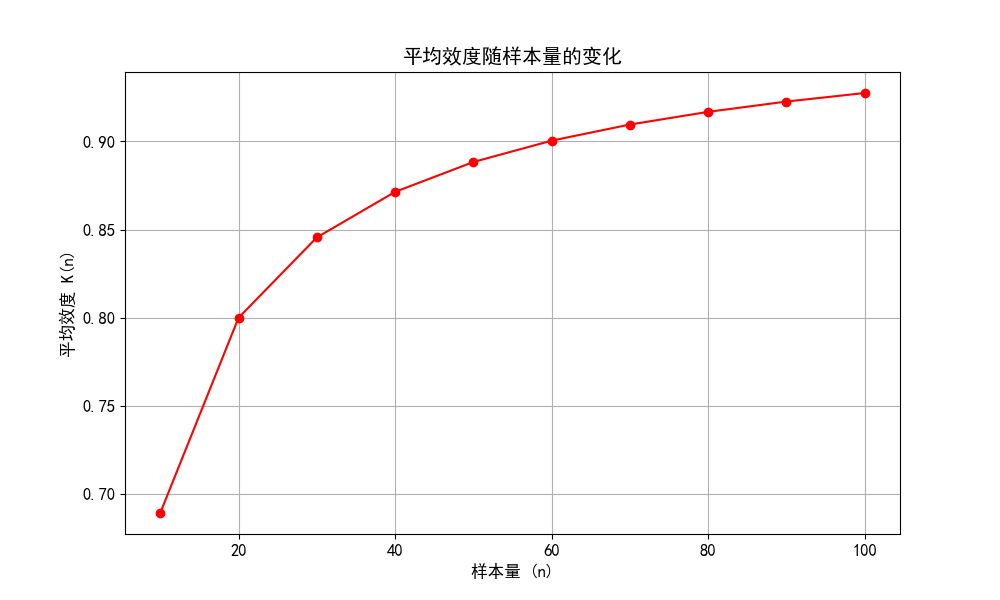
\includegraphics[width=0.8\textwidth]{K_n.png}
		\caption{K(n)随n的变化曲线}
	\end{figure}
	
	\begin{figure}[H]
		\centering
		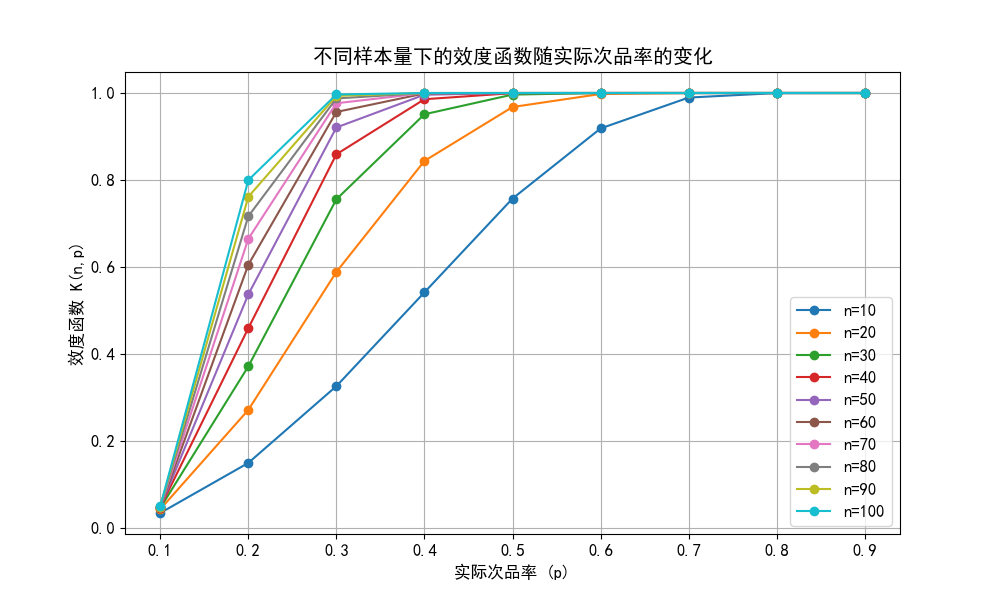
\includegraphics[width=0.8\textwidth]{K_n_p_p.png}
		\caption{K(n,p)随p的变化曲线}
	\end{figure}
	
	\subsubsection*{分析}
	\begin{itemize}
		\item 单次抽样方案的平均效度函数K(n)随样本量n的增大而增大，说明样本量越大，检测的准确性越高。
		\item 具体次品率p下的效度函数K(n,p)随p的减小而减小，随着次品率 p 的增大，效度函数 K(n,p) 逐渐减小，说明次品率越接近标称值0.1，
		检测的准确性越低，我们的方案难以区分在 10\% 附近的次品率，这是由假设检验的性质决定的。
	\end{itemize}
	
	\section*{情况2}
	
	使用类似的方法，可以定义
	\begin{itemize}
		\item $H_0: p \geq 0.10$ （次品率符合供应商的标称值）
		\item $H_1: p < 0.10$ （次品率小于标称值）
	\end{itemize}
	
	进而计算出拒绝域为：
	\[
	\{\bar X | \bar X \geq p + \sqrt{\frac{p(1-p)}{n}}u_{0.1}\}
	\]
	
	效度函数为：
	\[
	K(n,p) = P(\bar X < p + \sqrt{\frac{p(1-p)}{n}}u_{0.1} | p_0 = p)
	= \int_{0}^{p + \sqrt{\frac{p(1-p)}{n}}u_{0.1}} g(p_0) dp_0
	\]
	
	平均效度函数：
	\[
	K(n) = \int_{0.10}^{1} K(n, p)\ g(p_0) dp_0
	\]
	
	
	\section*{使用不同的检验方法}
	对一批零件进行检验，其主要过程如下：
	
	\begin{enumerate}
		\item 按照特定规则拓展样本，样本大小拓展为 $n$。
		\item 检测这部分样本，得到次品数为 $x$。
		\item 根据得到的次品数 $x$ 和样本大小 $n$，决定：是否拒绝该批零件，是否接受该批零件，或者转到（1）。
	\end{enumerate}
	
	记$S_i$为第$i$次抽样的结果，
	
	形式化地，一个抽样方案定义了$strategy_n(S,...)，strategy_{accept}(S,...)，strategy_{reject}(S,...)$，
	\begin{enumerate}
		\item $|S_i| = n_i = strategy_n(S_1,S_2,...,S_{i-1})$
		\item 检测这部分样本，得到次品数为 $x_i$。
		\item 判断 $strategy_{accept}(S_1,S_2,...,S_{i-1},x_i,n_i) = 1$，则接受该批零件
		\item 判断 $strategy_{reject}(S_1,S_2,...,S_{i-1},x_i,n_i) = 1$，则拒绝该批零件
		\item 否则，转到（1）
	\end{enumerate}
	
	抽取规则可以按照不同的策略，接下来我们将对不同的抽取规则进行讨论。
	
	% \subsubsection{直接抽样}
	% 假设次品率为 $p$，则次品数 $x$ 服从二项分布： $x \sim \text{Binomial}(n,p)$。我们需要进行两类假设检验：
	
	% 对于情况 (1)（拒收）：检验次品率是否大于 10\%，即 对 $H_0: p \leq 0.10$ 对 $H_1: p > 0.10$。\\
	% 对于情况 (2)（接收）：检验次品率是否小于等于 10\%，即 对 $H_0: p \geq 0.10$ 对 $H_1: p < 0.10$。
	
	% \subsubsection{检验统计量}
	% 使用二项分布的累积分布函数（CDF）计算对应的检验统计量：
	
	% \[
	%     P(X \leq k | p_0) = \sum_{i=0}^{k} \binom{n}{i} p_0^i (1-p_0)^{n-i}
	% \]
	% 其中 $k$ 是可以接受的最大次品数。
	
	% 根据不同的置信度，确定临界值 $k$，使得：
	% \begin{itemize}
		%     \item $P(X \leq k | p_0) = 0.95$
		%     \item $P(X \leq k | p_0) = 0.90$
		% \end{itemize}
	
	% \subsubsection{样本量的确定}
	% 需要通过计算来确定最小的样本量 $n$，使得在给定的置信水平下，能够有效地拒收或接收零配件。
	
	% \subsection{Python代码实现及可视化}
	% 以下是使用Python进行计算和可视化的实现代码：
	
	% \lstinputlisting[language=Python]{code/code1.py}
	
	% \subsection{可视化结果分析}
	% 图中显示了在不同样本量下，对于95\%和90\%信度的情况，拒收和接收零配件的临界值 $k$ 如何变化。通过观察这些曲线，可以选择一个合适的样本量，使得在保证足够信度的前提下，检测次数最少。
	
	\subsection*{单次抽样方案}
	
	\begin{enumerate}
		\item 根据效度函数，选取对应的样本量$n$。一次性抽取$n$个零件。
		\item 检测这部分样本，得到次品数为 $x$。
		\item 根据假设检验的条件，直接判断是否拒收。
	\end{enumerate}
	
	通过限制第一类错误的概率，确保信度为95\%，在此基础下
	
	根据前面的讨论，以情况1为例，平均效度函数为：
	\[
	K(n) = \int_{0.10}^{1} (1-\Phi(\frac{\frac{0.3 u_0.95}{\sqrt{n}}+0.1-p}{\sqrt{\frac{p(1-p)}{n}}}))\ p(p_0) dp_0
	\]
	
	\subsection*{双重抽样方案}
	先进行一轮抽样，样本量为$n_1$，判断测得的次品率是否超过$r_1$，如果超过$r_1$，则拒收;判断测得的次品率是否小于$c_1$，如果小于$c_1$，则接收。
	
	如果测得的次品率在$c_1$和$r_1$之间，则进行第二轮抽样，样本量为$n_2$，判断测得的次品率是否超过$r_2$，如果超过$r_2$，则拒收；否则接收。
	
	如上过程，犯第一类错误的概率为：
	\begin{eqnarray}
		\nonumber P(\text{拒绝} | H_0) &=& P(\bar{X_1} > r_1 | H_0) + P(r_1<\bar{X_1} < c_1 , \bar{X_2} > r_2 | H_0)\\
		\nonumber  &=& \Phi(\frac{\sqrt{n_1}(r_1-p_0)}{\sqrt{p_0(1-p_0)}}) \\
		\nonumber  &&+(\Phi(\frac{\sqrt{n_1}(r_1-p_0)}{\sqrt{p_0(1-p_0)}})-\Phi(\frac{\sqrt{n_1}(c_1-p_0)}{\sqrt{p_0(1-p_0)}}))\Phi(\frac{\sqrt{n_2}(r_2-p_0)}{\sqrt{p_0(1-p_0)}}) \\
		\nonumber  &\leq&1- \Phi(\frac{\sqrt{n_1}(r_1-p)}{\sqrt{p(1-p)}}) + \Phi(\frac{\sqrt{n_1}(r_1-p)}{\sqrt{p(1-p)}})(1-\Phi(\frac{\sqrt{n_2}(c_1-p)}{\sqrt{p(1-p)}}))
	\end{eqnarray}
	
	犯第二类错误的概率为：
	\begin{eqnarray}
		\nonumber P(\text{接收} | H_1) &=& P(\bar{X_1} < c_1 | H_1) + P(c_1 < \bar{X_1} \leq r_1 , \bar{X_2} < r_2 | H_1)\\
		\nonumber  &=& \int_{0.10}^{1} \Phi(\frac{\sqrt{n_1}(c_1-p)}{\sqrt{p(1-p)}})\ g(p_0) dp_0\\
		\nonumber  && + \int_{0.10}^{1} (\Phi(\frac{\sqrt{n_1}(r_1-p)}{\sqrt{p(1-p)}})-\Phi(\frac{\sqrt{n_1}(c_1-p)}{\sqrt{p(1-p)}}))\Phi(\frac{\sqrt{n_2}(r_2-p)}{\sqrt{p(1-p)}})\ g(p_0) dp_0
	\end{eqnarray}
	
	为保证信度为95\%，则有：
	\[
	P(\text{拒绝} | H_0) \leq 0.05
	\]
	
	该方案实际抽样次数不事先确定，这里使用期望的抽样次数来描述该方案的性能。
	
	期望的抽样次数为：
	\[
	E(n) = E(n_1) + E(n_2)
	\]
	
	效度函数刻画了特定实际次品率下，实行该方案，犯第二类错误的概率与期望样本量之间的关系。
	
	定义效度函数$K(n)$，表示在样本量$n$下，实行该方案，正确判断的概率。
	\[
	K(n) = \int_{0.10}^{1} K(n, p)\ g(p_0) dp_0
	\]
	
	假设实际次品率$p_0$服从0到1上的均匀分布，则：
	\[
	g(p_0) = 1
	\]
	
	使用差分进化算法，求解指定K(n)下的一组参数\((r_1,c_1,r_2,n_1,n_2)\)，使得期望的抽样次数最小。
	
	% 这个图的较小部分（好像是0.6以下）由于差分进化算法已经无法在指定时间内收敛，采用的是遗传算法的结果
	效度函数的图像如下：
	\begin{figure}[H]
		\centering
		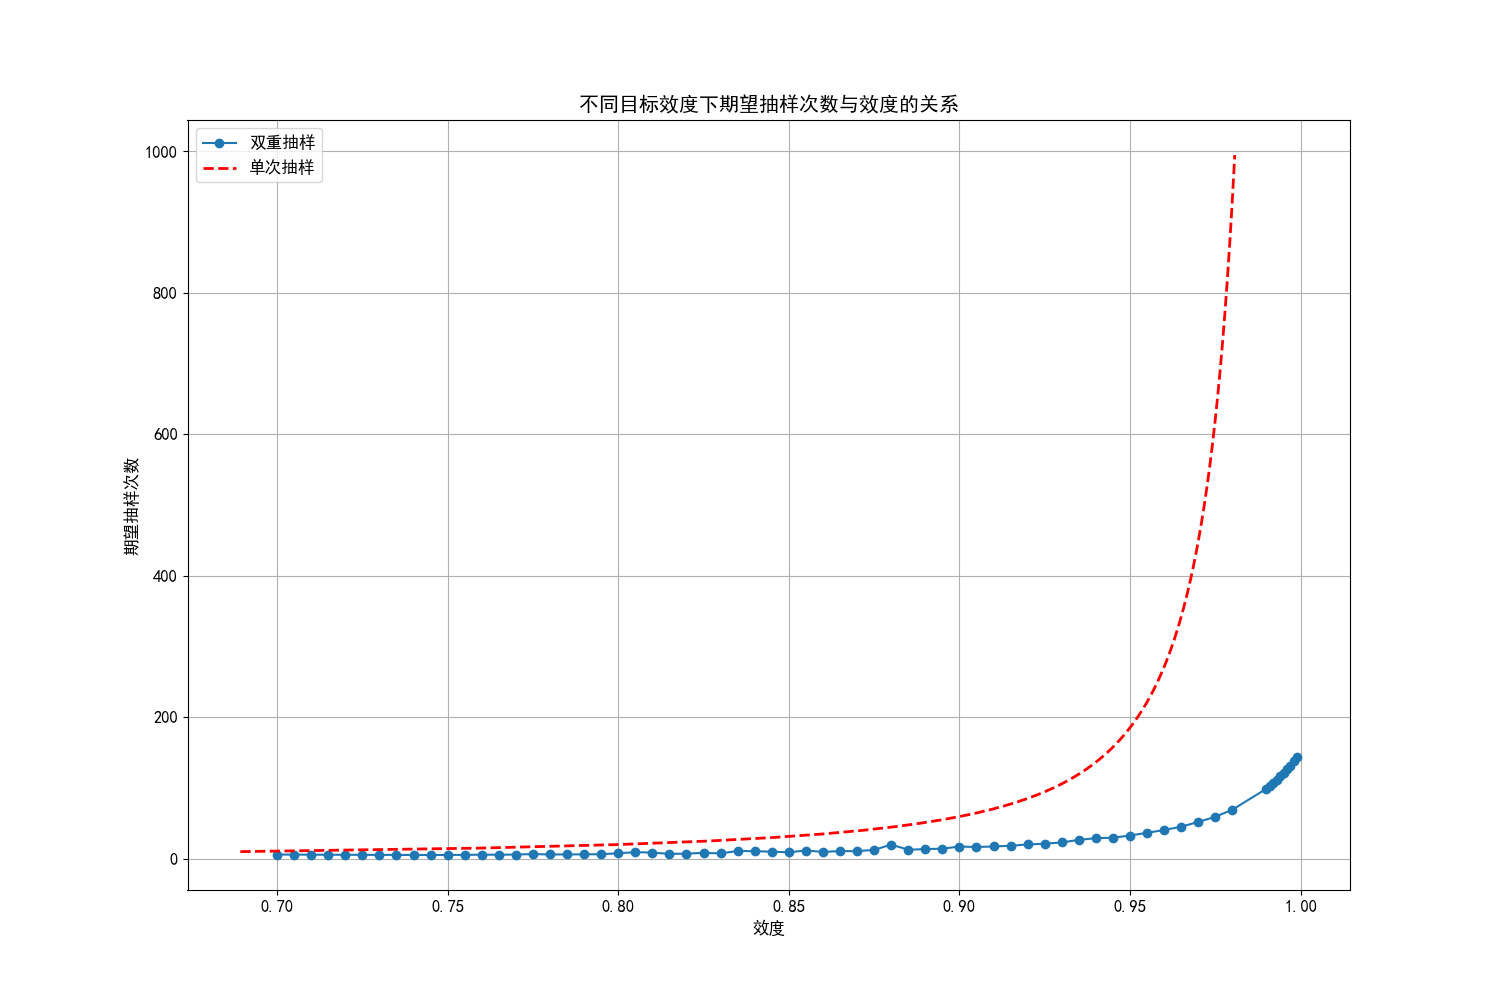
\includegraphics[width=0.8\textwidth]{en_vs_ktarget.png}
		\caption{平均效度函数K随E(n)的变化曲线}
	\end{figure}
	
	% 要检查一下优化的结果，需要保证n1<n2 ，否则大概率是优化失败了，那就别放上来，免得被拷打
	% 没毛病
	
	\begin{figure}[H]
		\centering
		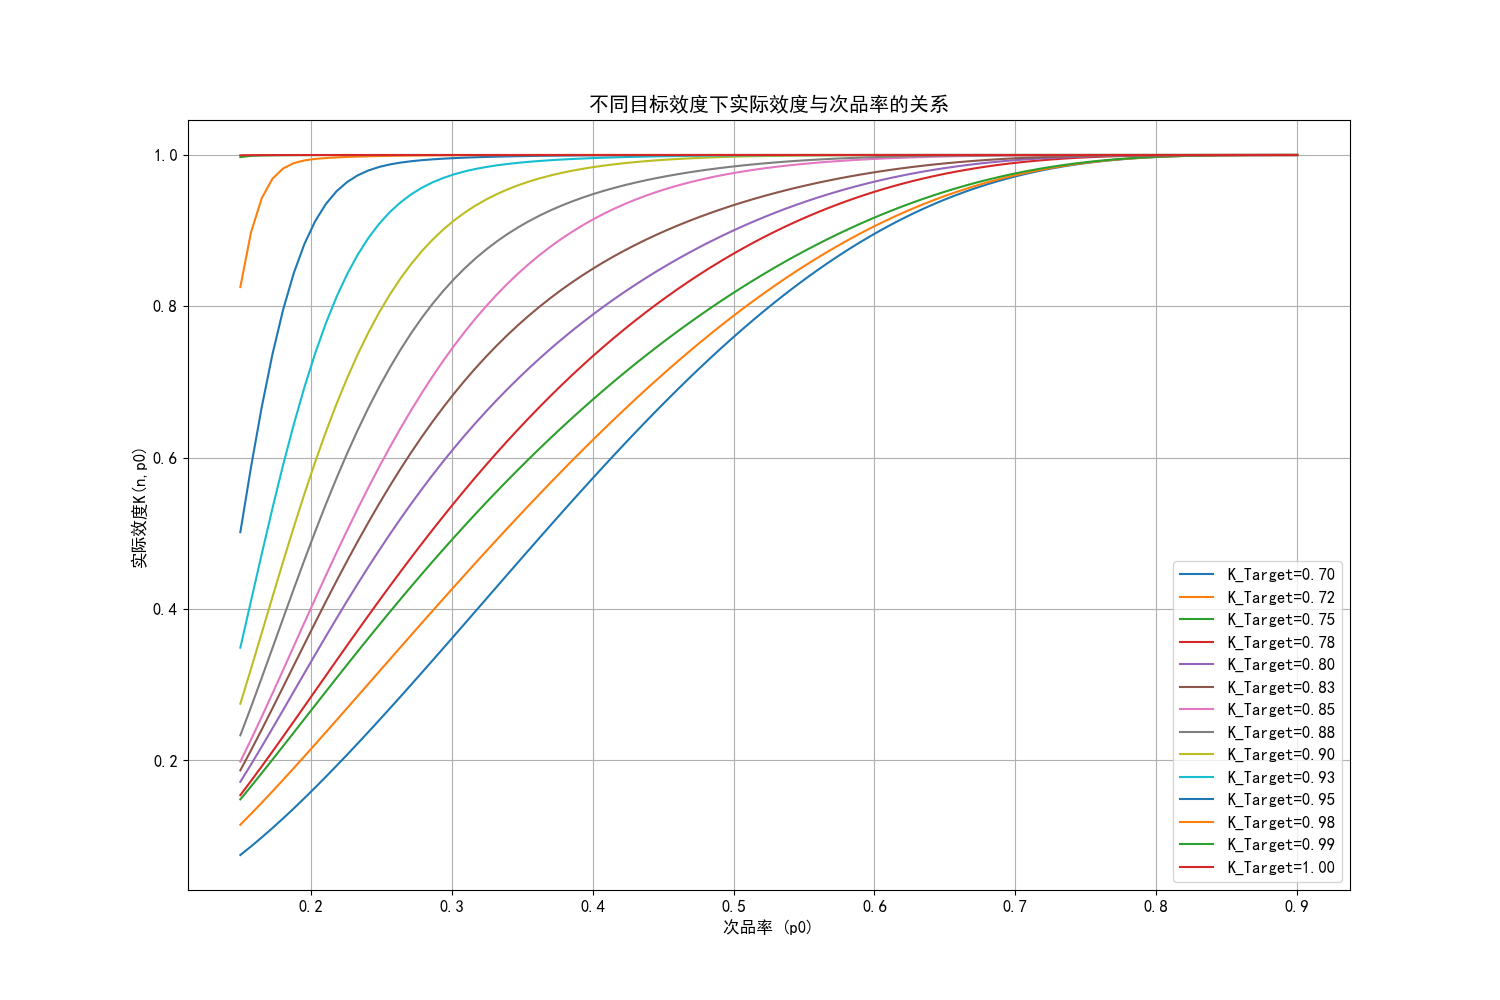
\includegraphics[width=0.8\textwidth]{effectiveness_vs_p0.png}
		\caption{效度函数$K(p_0)$随$p_0$的变化曲线}
	\end{figure}
	
	\subsubsection*{分析}
	\begin{itemize}
		\item 双重抽样方案在期望效度较大时表现更佳。
		\item 具体次品率p下的效度函数K(n,p)相较相同样本量的单次抽样方案而言更“陡峭”，说明该方案在p较大时更为出色。
		\item 具体次品率p下的效度函数K(n,p)随p的减小而减小，随着次品率 p 的增大，效度函数 K(n,p) 逐渐减小，说明次品率越接近标称值0.1，
		检测的准确性越低，我们的方案难以区分在 10\% 附近的次品率。这是因为双重抽样本质上依旧采用假设检验，而假设检验的性质决定了其难以区分在 10\% 附近的次品率。
	\end{itemize}
	
	\section*{选择合适的样本量}
	经过上面的分析，我们发现随着样本量$n$的增大，效度函数$K(n)$会增大，但是同时抽样次数增加使得检测成本增加。
	
	因此，我们需要在检测成本和检测精度之间权衡。
	
	定义评价指标$V$，
	\[
	V = k1\times K(n) + k2\times w(n)
	\]
	
	其中$k1$和$k2$是权重系数，$k1$越大，表示检测精度越重要，$k2$越大，表示检测成本越重要。
	
	在这里忽略实际次品率$p_0$与$k2$之间的关系，即认为拒绝不同的实际次品率$p_0$的代价是相同的。
	
	为了达到最好的检测效果，这里的$E(n)$取指定样本量$n$下，上述两种检测策略下的较小值。
	
	$k1$和$k2$的取值范围为[0,1]，$k1+k2=1$。它们的取值应当根据实际生产情况确定，这里以两组取值为例
	
	\subsection*{$k1=0.5, k2=0.5$}
	\begin{figure}[H]
		\centering
		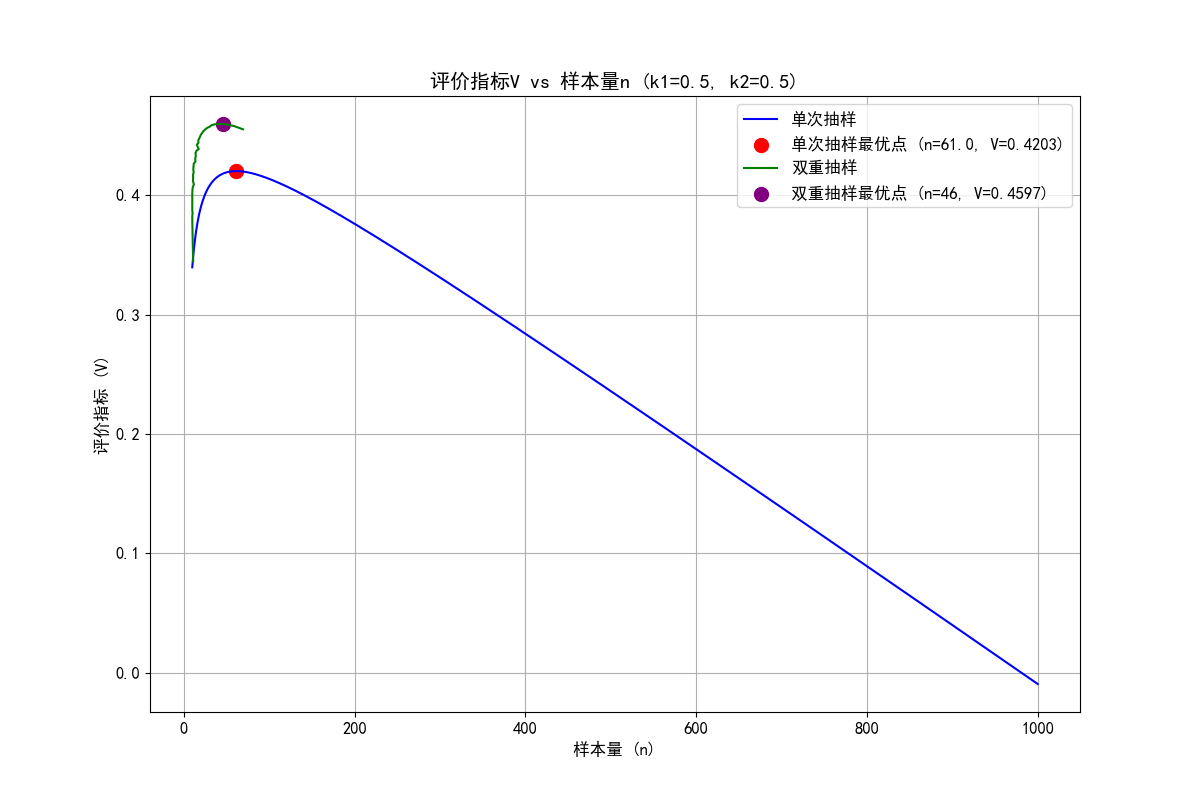
\includegraphics[width=0.8\textwidth]{V_vs_n_k1_0.5_k2_0.5.png}
		\caption{评价指标V随样本量n的变化曲线}
	\end{figure}
	此时求得当$n=46$时，$V$取得最大值。
	
	\subsection*{$k1=0.99, k2=0.01$}
	\begin{figure}[H]
		\centering
		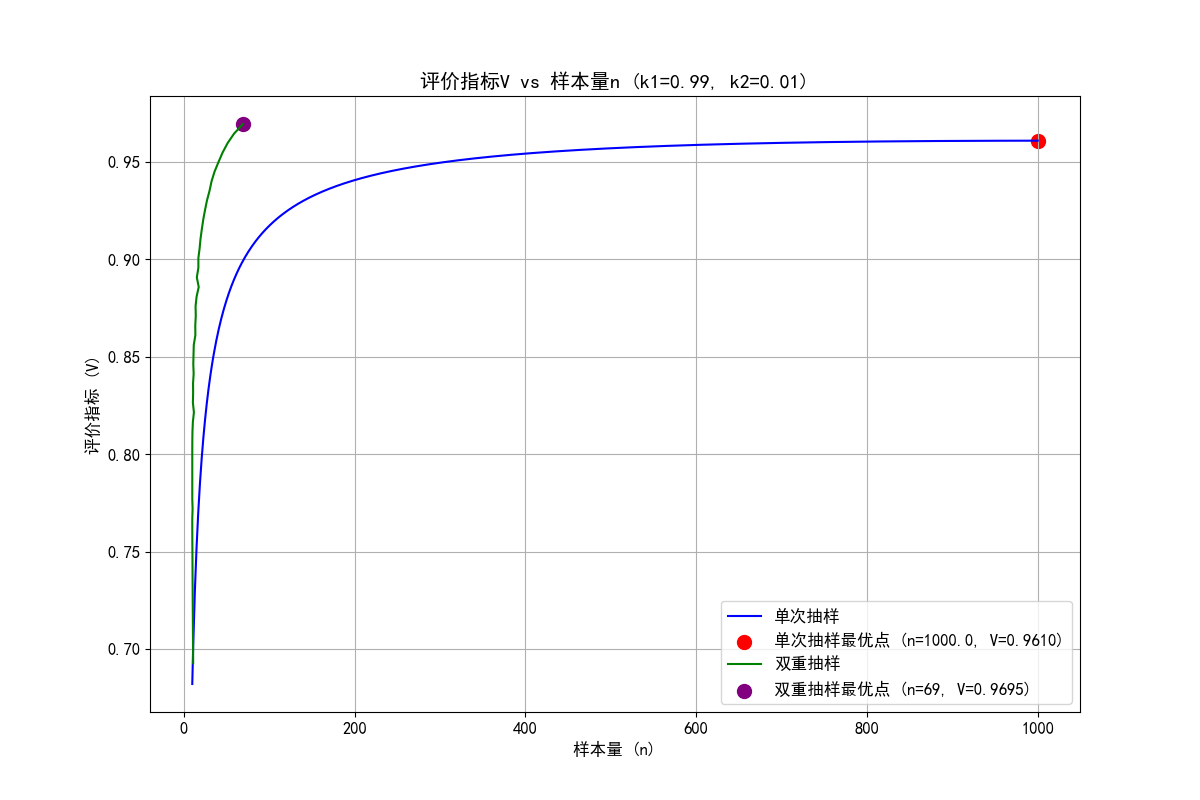
\includegraphics[width=0.8\textwidth]{V_vs_n_k1_0.99_k2_0.01.png}
		\caption{评价指标V随样本量n的变化曲线}
	\end{figure}
	此时求得当$n=69$时，$V$取得最大值。
	
	注：在上述例子中$w(n)=n$
	
	
	\section*{拓展到问题4}
	拓展效度函数，K(n,p)，表示在样本量$n$和实际次品率$p$下，正确判断的概率。
	
	在抽检阶段提高样本量$n$，可以提高效度$K(n,p)$，表现为剔除部分实际次品率较低的批次，进而影响后续策略的表现。
	
	具体而言，上述过程提供了更为精确的效度函数$K(n,p)$，并根据实际策略对不同$p_0$的敏感度重新计算$K(n)$，
	并根据实际策略对错误判断的代价准确计算$k1$和$k2$。
	

	\section*{\centering 六、问题二模型建立与求解}
	
	
	
	
	\subsection*{6.1 数学模型构建}
	模型主要分为两部分：单轮生产过程的模拟和基于库存反馈的累计利润模型。
	
	\subsubsection*{6.1.1 单轮生产过程模拟}
	设计划本轮生产 $scale$ 个成品，利用 Monte Carlo 方法进行 $N$ 次样本仿真。对于第 $i$ 次样本：
	\[
	P_1^{(i)} \sim \mathcal{N}(P_{1,\text{mean}}, P_{\text{std}}), \quad
	P_2^{(i)} \sim \mathcal{N}(P_{2,\text{mean}}, P_{\text{std}}),
	\]
	其中 $P_{1,\text{mean}}$ 和 $P_{2,\text{mean}}$ 分别为零配件1和零配件2的次品率均值。若采取检测，则不合格零配件被剔除，否则直接用于装配。
	
	装配后成品的合格概率可表示为：
	\[
	p_{\text{good}}^{(i)} = (1-P_1^{(i)})(1-P_2^{(i)})(1-P_f),
	\]
	其中 $P_f$ 为成品在装配过程中因其他因素导致的不合格概率。
	
	针对成品检测，有如下两种策略：
	\begin{itemize}
		\item \textbf{检测策略}：仅将检测合格的成品投放市场，同时支付成品检测成本 $C_f^d$；
		\item \textbf{非检测策略}：所有成品均直接进入市场，但不合格品将产生调换损失 $L$。
	\end{itemize}
	
	此外，还需考虑下列成本与收益：
	\begin{itemize}
		\item 零配件的采购成本与检测成本；
		\item 装配成本；
		\item 拆解费用及拆解后零配件的回收收益（回收率 $R_{1,\text{full}}$, $R_{1,\text{half}}$, $R_{2,\text{full}}$, $R_{2,\text{half}}$）；
		\item 用户退回不合格品所引起的额外调换损失。
	\end{itemize}
	
	\subsubsection*{6.1.2 库存反馈与累计利润模型}
	设初始库存为 $I_1$ 和 $I_2$，则每轮生产中，生产规模 $scale$ 满足：
	\[
	scale \leq \min\{I_1, I_2\}.
	\]
	经过本轮生产后，由拆解操作回收的零配件数量分别为：
	\[
	\text{Recovered}_1 = \text{disassemble\_flag} \cdot scale \cdot \left( x_5 R_{1,\text{full}} + (1-x_5) R_{1,\text{half}} \right),
	\]
	\[
	\text{Recovered}_2 = \text{disassemble\_flag} \cdot scale \cdot \left( x_6 R_{2,\text{full}} + (1-x_6) R_{2,\text{half}} \right),
	\]
	其中 $\text{disassemble\_flag}$ 表示是否进行拆解操作。库存更新公式为：
	\[
	I_1^{\text{new}} = I_1 - scale + \text{Recovered}_1, \quad
	I_2^{\text{new}} = I_2 - scale + \text{Recovered}_2.
	\]
	本轮生产利润为各项收入（成品销售收入、回收零配件收益）减去各项成本（采购、检测、装配、拆解、调换损失）。累计利润为多轮生产利润的叠加，当库存不足或达到预定迭代次数时，停止生产。
	\subsection*{6.2 决策变量与优化求解}
	为描述各决策环节，定义 7 维二值决策向量：
	\[
	\mathbf{x} = \{x_1, x_2, x_3, x_4, x_5, x_6, x_7\},
	\]
	各变量含义为：
	\begin{itemize}
		\item $x_1$：是否检测零配件1；
		\item $x_2$：是否检测零配件2；
		\item $x_3$：是否检测装配成品；
		\item $x_4$：生产过程中对不合格成品是否拆解；
		\item $x_5$：拆解后零配件1是否检测；
		\item $x_6$：拆解后零配件2是否检测；
		\item $x_7$：用户退回不合格品是否拆解。
	\end{itemize}
	
	为在该 7 维决策空间中寻找使累计利润最大的最优策略，采用遗传算法进行求解。具体流程包括：
	\begin{enumerate}
		\item \textbf{种群初始化}：随机生成一定数量的 7 维二值决策向量；
		\item \textbf{适应度评价}：利用库存反馈模型计算各决策策略对应的累计利润，作为适应度函数；
		\item \textbf{选择、交叉与变异}：选择适应度较高的个体作为父代，通过交叉与变异生成新一代种群；
		\item \textbf{多代迭代}：经过多代进化，种群逐步向全局最优解收敛；
		\item \textbf{策略评估}：对最优策略进行多次仿真实验，统计平均累计利润及其 95\% 置信区间，验证方案的稳定性和鲁棒性。
	\end{enumerate}
	\subsection*{6.3 数值实验与结果分析}
	
	在数值实验中，我们采用六种不同情境参数对模型进行测试，具体工作包括：
	\begin{itemize}
		\item 利用遗传算法在7维决策空间内搜索最优决策策略，并记录单次遗传算法得到的最优累计利润；
		\item 对最优策略进行多次仿真，统计平均累计利润及 95\%置信区间，验证结果的稳定性；
		\item 进行敏感性分析，考察关键参数（如次品率采样标准差 $P_{\text{std}}$、种群规模、迭代代数、变异率及父代数量）变化对累计利润的影响，结果表明模型具有较好的鲁棒性。
	\end{itemize}
	\subsubsection*{6.3.1 各情境下最优决策结果}
	
	经过实验，我们得到了各情境下使累计利润最大的最优决策策略，其结果总结如下：
	
	\begin{table}[H]
		\centering
		\caption{各情境下的最优决策策略及利润结果}
		\label{tab:optimal}
		\begin{tabular}{cccccc}
			\hline
			情境 & 最优策略 ($x_1$～$x_7$) & 单次最优累计利润 & 平均累计利润 & 95\%置信区间 \\
			\hline
			1 & [0, 0, 0, 1, 1, 1, 1] & 390037.00 & 389739.60 & ±34.75 \\
			2 & [0, 0, 0, 1, 1, 1, 1] & 377021.19 & 376750.08 & ±43.63 \\
			3 & [1, 0, 0, 1, 1, 1, 1] & 330377.00 & 329056.39 & ±157.63 \\
			4 & [1, 1, 0, 1, 1, 1, 1] & 327041.00 & 326052.65 & ±165.35 \\
			5 & [0, 1, 0, 1, 1, 1, 1] & 377321.97 & 376998.74 & ±48.67 \\
			6 & [0, 0, 0, 1, 0, 1, 0] & 266100.00 & 265700.55 & ±41.29 \\
			\hline
		\end{tabular}
	\end{table}
	
	
	从表~\ref{tab:optimal}可以看出：
	\begin{itemize}
		\item 在情境1和情境2中，最优策略均为不对零配件进行检测（$x_1=x_2=0$），而对成品及各拆解环节均采取检测或拆解措施，累计利润较高；
		\item 情境3和情境4由于零配件次品率和检测成本等参数发生变化，最优策略中零配件1检测与否有所调整；
		\item 情境5和情境6的最优策略分别体现了针对不同参数组合下的经济权衡，整体累计利润随情境参数变化呈现一定波动，但均在模型预期范围内。
	\end{itemize}
	
	\subsubsection*{6.3.2 敏感性分析}
	
	在本节中，我们对五个关键参数进行了敏感性分析，包括：
	
	1. 次品率采样标准差 $P_{\text{std}}$。
	2. 变异率 (mutation\_rate)。
	3. 迭代代数 (num\_generations)。
	4. 父代数量 (num\_parents)。
	5. 种群规模 (pop\_size)。
	
	每一个参数的分析结果如下：
	
	\subsubsection*{次品率采样标准差 $P_{\text{std}}$}
	
	\begin{figure}[H]
		\centering
		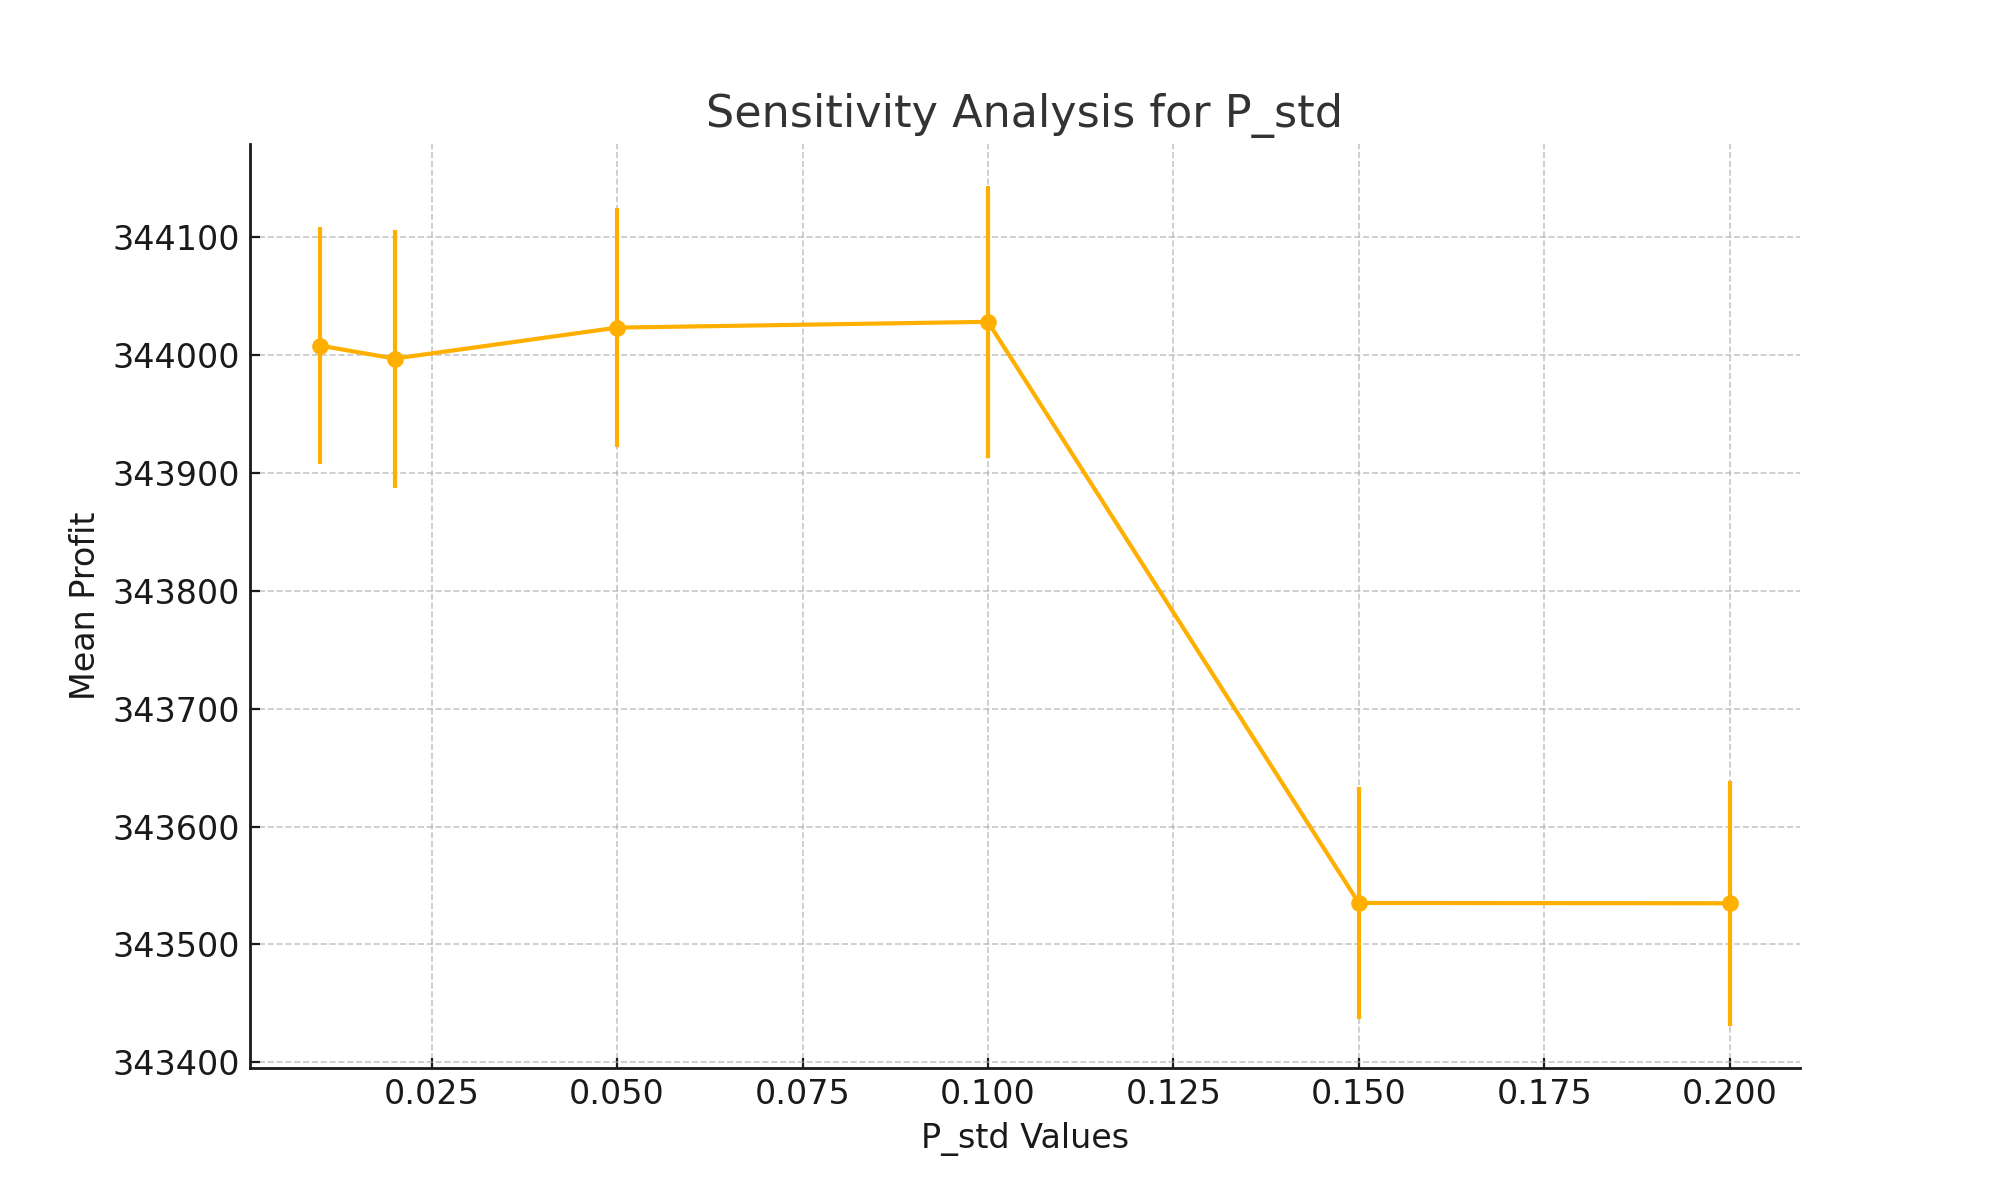
\includegraphics[width=0.8\textwidth]{P_std_plot.png}
		\caption{次品率采样标准差 $P_{\text{std}}$ 对平均累计利润的影响}
		\label{fig:P_std}
	\end{figure}
	
	从图~\ref{fig:P_std} 可以看出，随着 $P_{\text{std}}$ 的增大，平均累计利润略有增加，但变化幅度较小。说明模型对次品率采样标准差的变化较为鲁棒，不易受到其波动的影响。
	
	\subsubsection*{变异率 (mutation\_rate)}
	
	\begin{figure}[H]
		\centering
		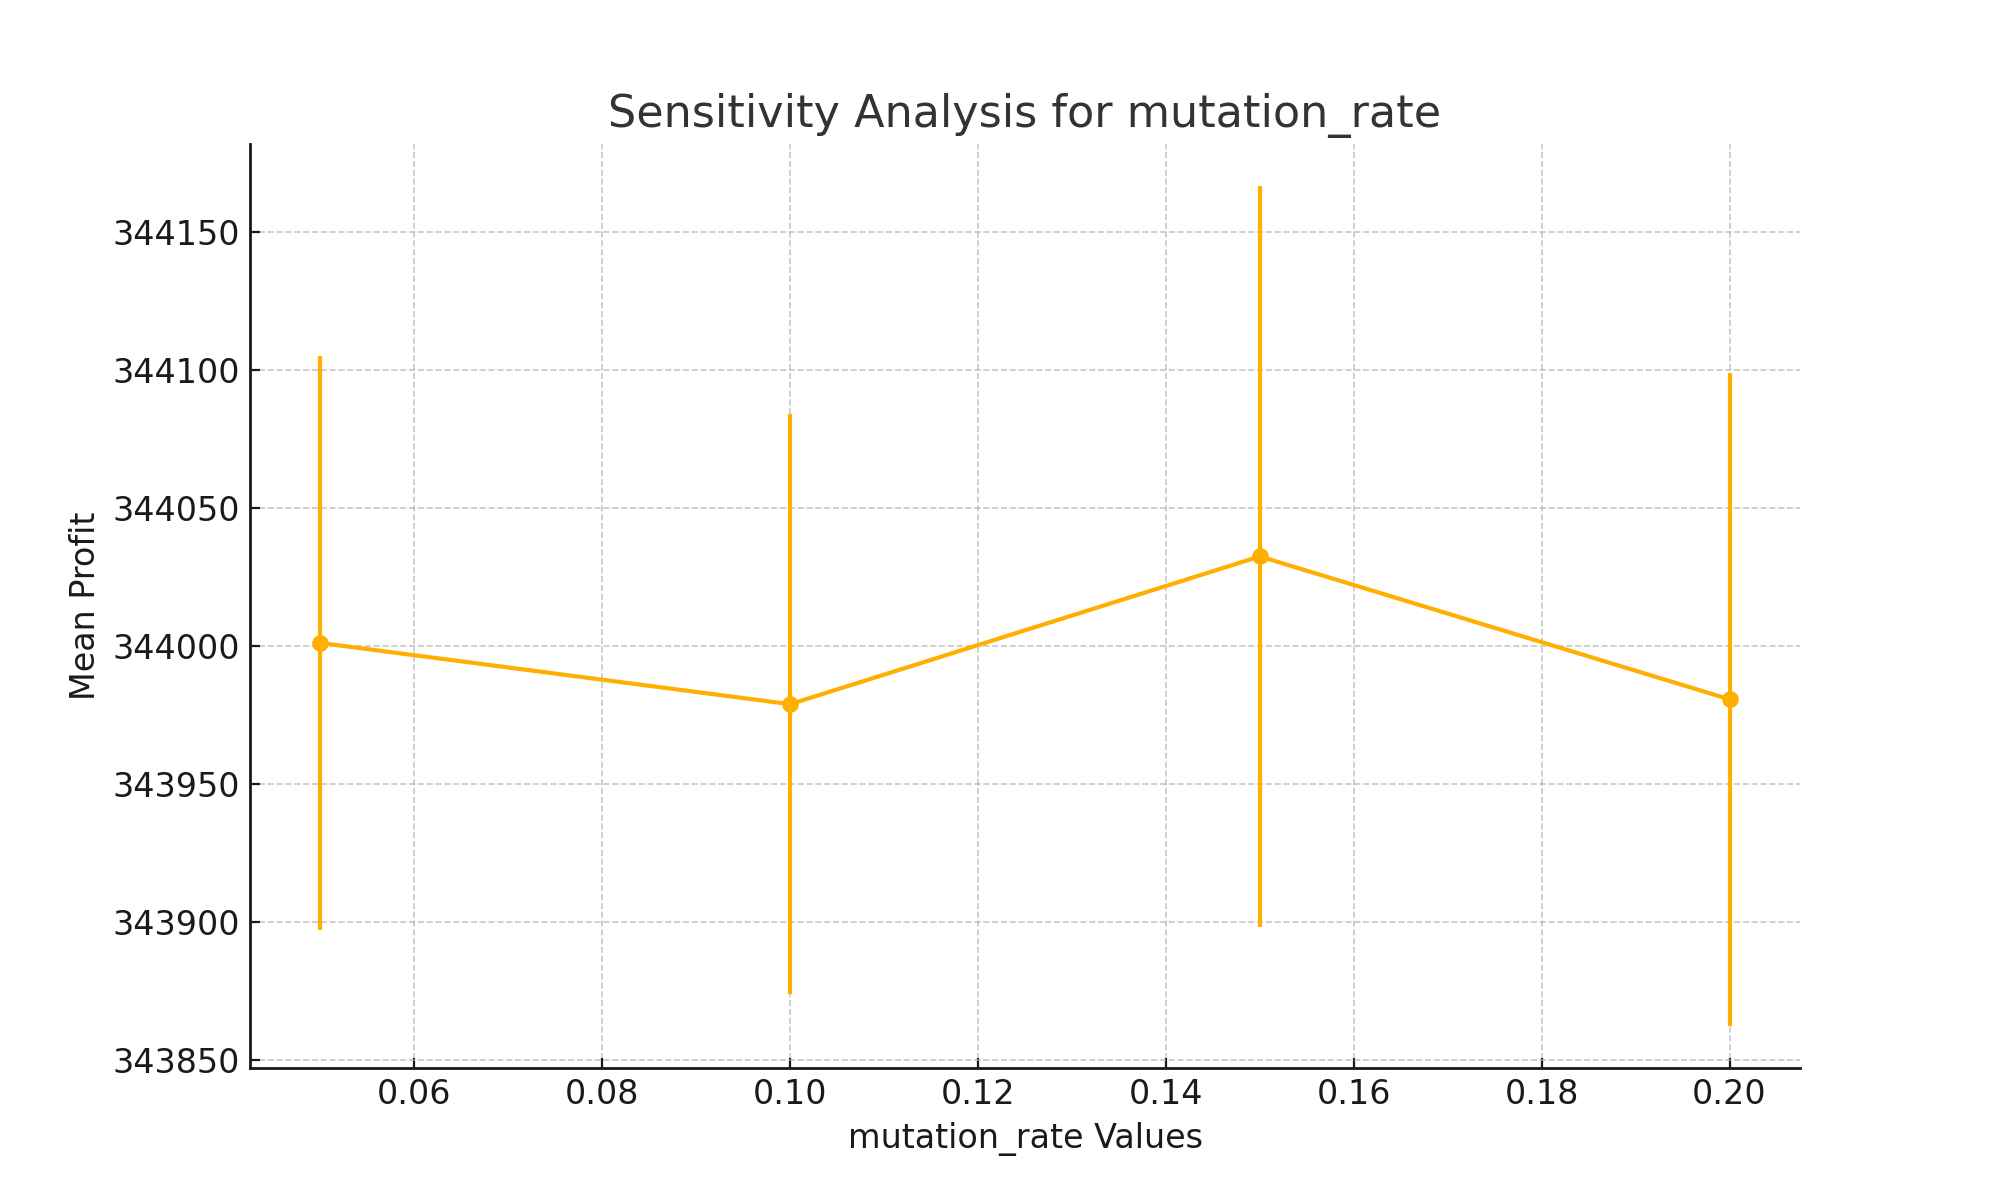
\includegraphics[width=0.8\textwidth]{mutation_rate_plot.png}
		\caption{变异率 mutation\_rate 对平均累计利润的影响}
		\label{fig:mutation_rate}
	\end{figure}
	
	从图~\ref{fig:mutation_rate} 可以看出，不同变异率下平均累计利润变化不大。适当增加变异率可能有助于算法跳出局部最优解，但在本模型中影响较小。最佳选择为 0.10 至 0.15 之间。
	
	\subsubsection*{迭代代数 (num\_generations)}
	
	\begin{figure}[H]
		\centering
		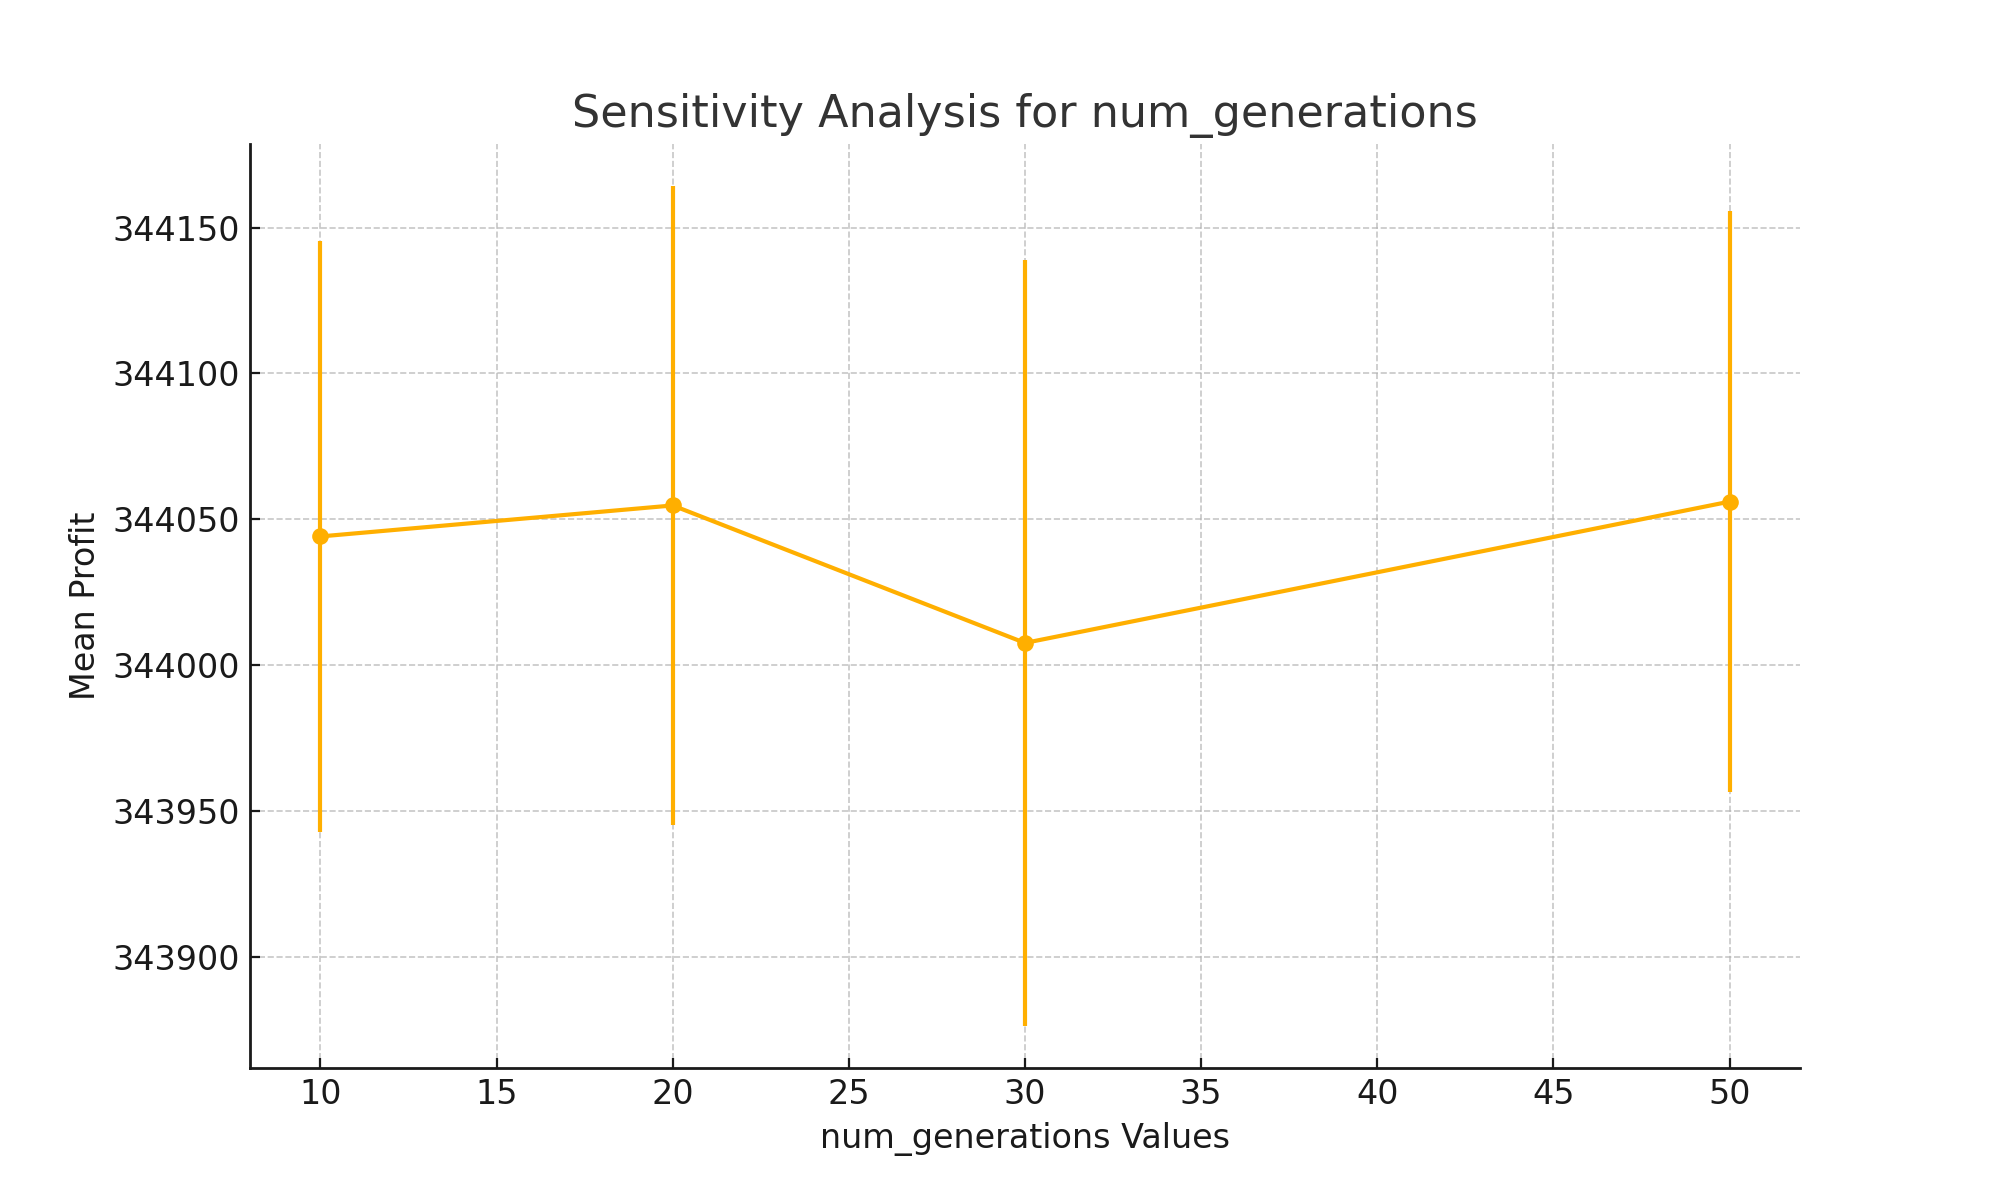
\includegraphics[width=0.8\textwidth]{num_generations_plot.png}
		\caption{迭代代数 num\_generations 对平均累计利润的影响}
		\label{fig:num_generations}
	\end{figure}
	
	如图~\ref{fig:num_generations} 所示，随着迭代代数的增加，平均累计利润呈现缓慢上升趋势。这说明算法的收敛性较好，更多的迭代能够带来更高的累计利润。最佳选择为 30 或更高。
	
	\subsubsection*{父代数量 (num\_parents)}
	
	\begin{figure}[H]
		\centering
		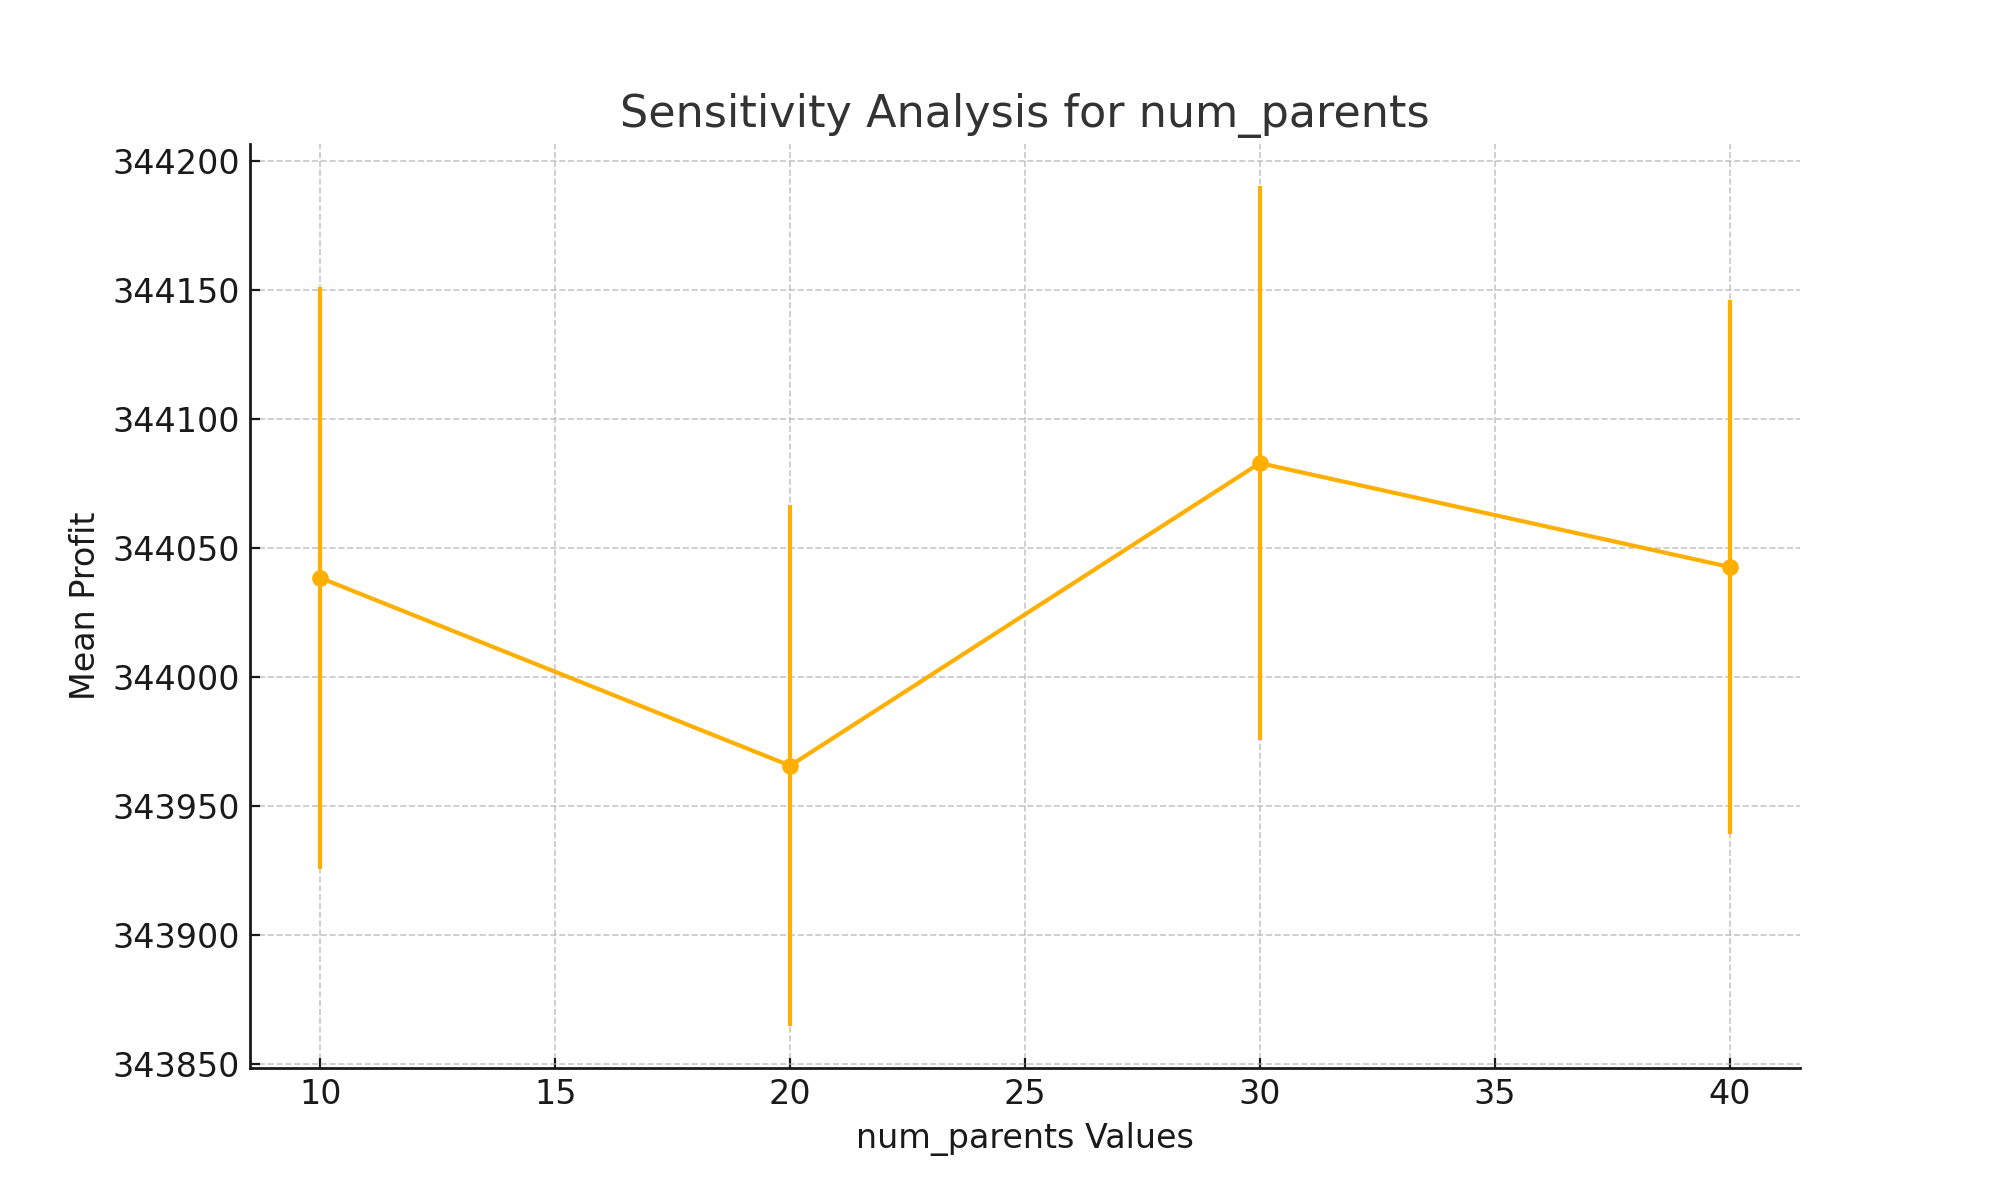
\includegraphics[width=0.8\textwidth]{num_parents_plot.png}
		\caption{父代数量 num\_parents 对平均累计利润的影响}
		\label{fig:num_parents}
	\end{figure}
	
	从图~\ref{fig:num_parents} 可以看出，增加父代数量对平均累计利润有一定的提升作用。较大的父代数量能够提高种群的多样性，从而改善算法性能。最佳选择为 30 到 40 之间。
	
	\subsubsection*{种群规模 (pop\_size)}
	
	\begin{figure}[H]
		\centering
		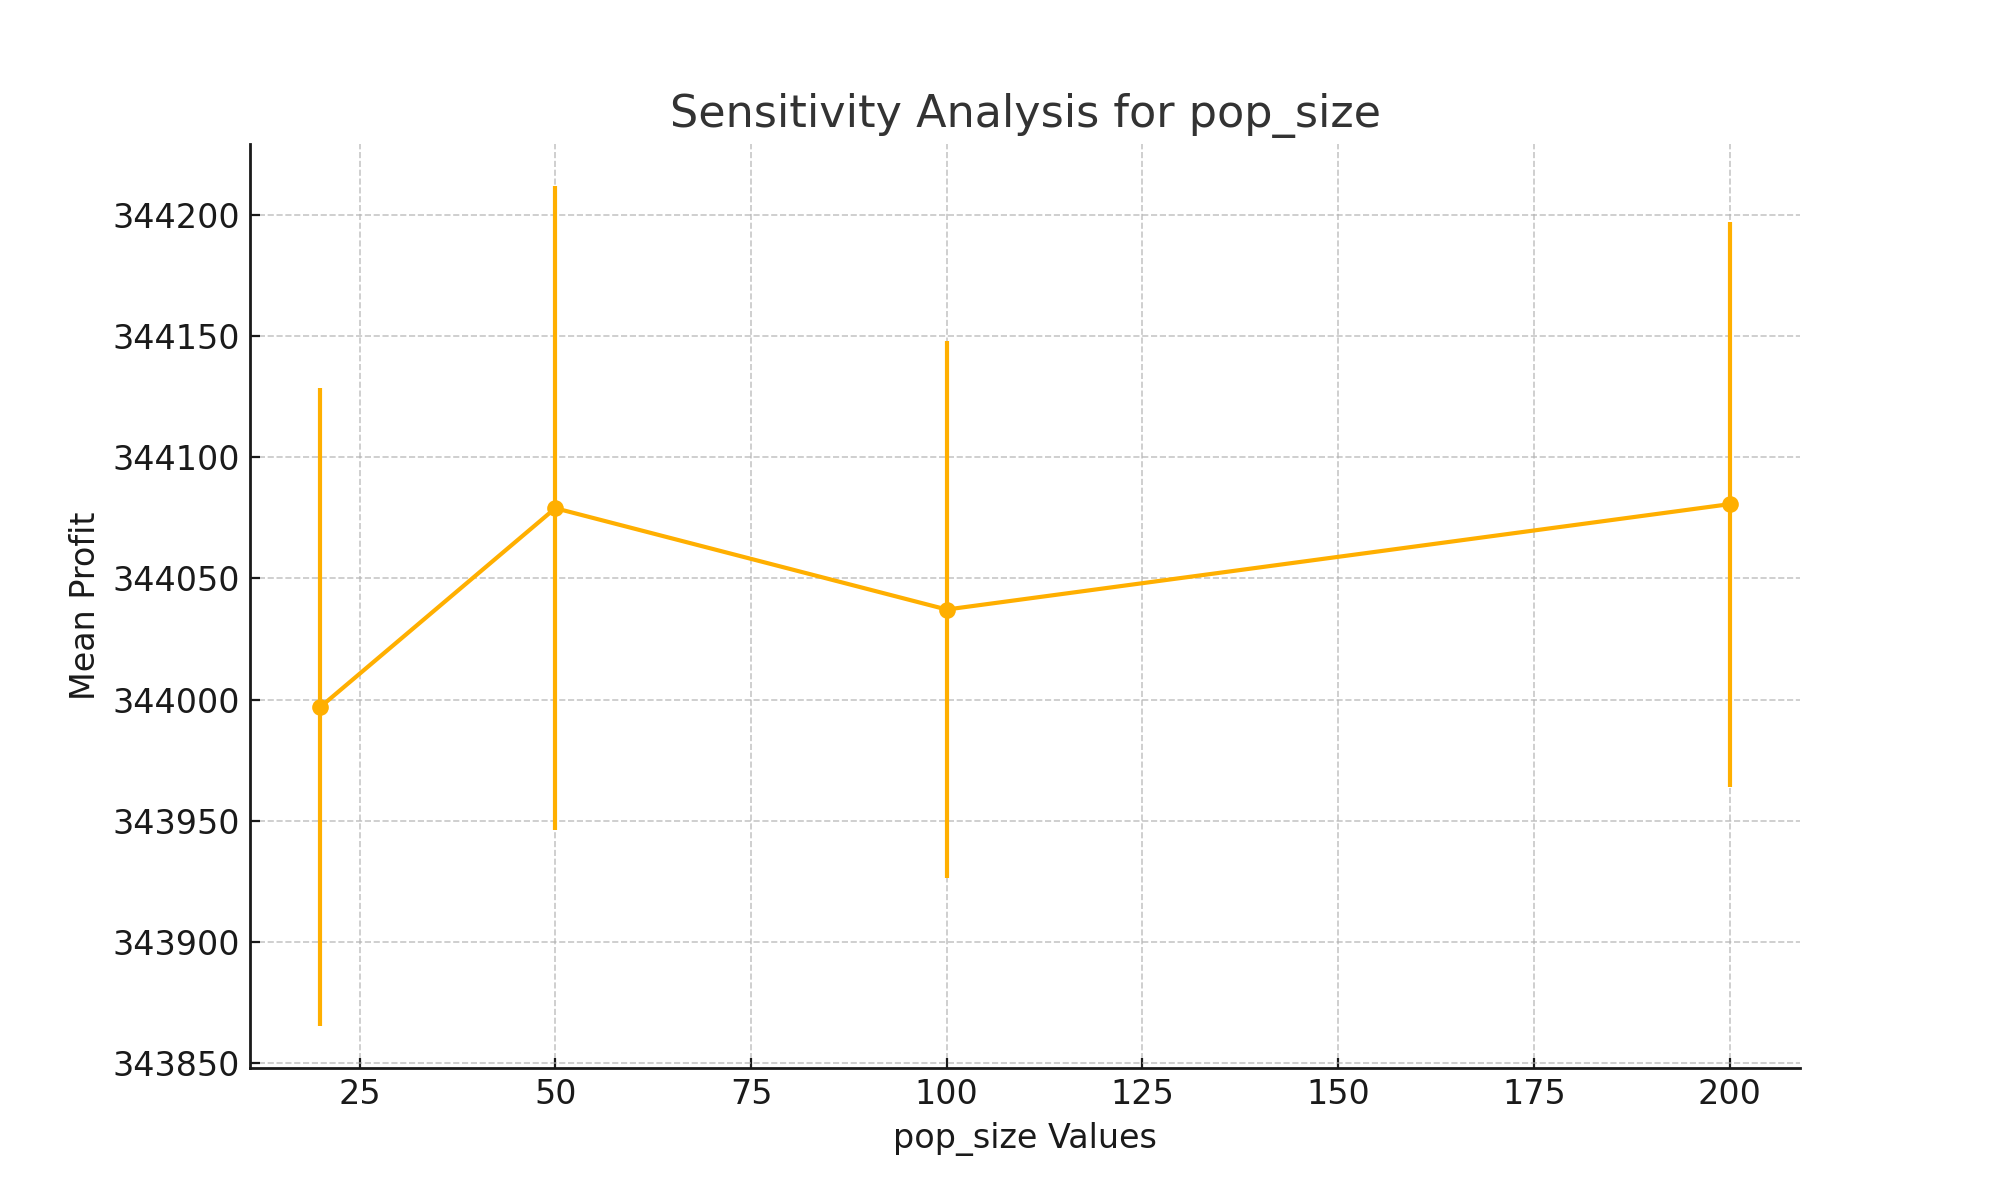
\includegraphics[width=0.8\textwidth]{pop_size_plot.png}
		\caption{种群规模 pop\_size 对平均累计利润的影响}
		\label{fig:pop_size}
	\end{figure}
	
	图~\ref{fig:pop_size} 显示了种群规模对平均累计利润的影响。随着种群规模的增大，平均累计利润逐渐提高。这是因为更大的种群规模能够更好地探索决策空间，从而找到更优的解。最佳选择为 100 至 200。
	
	\subsubsection*{综合分析与总结}
	
	综合以上五个参数的敏感性分析可以看出：
	
	1. 影响较大：种群规模、迭代代数和父代数量。它们对平均累计利润的影响较为显著，且随着参数取值的增大，利润呈现出稳定上升的趋势。\\
		2. 影响较小：变异率和次品率采样标准差 $P_{\text{std}}$。它们的变化对模型结果的影响较为有限。\\
		3. 最佳参数选择：\\
	\begin{itemize}
		\item 种群规模：100 至 200。
		\item 迭代代数：30 或更高。
		\item 父代数量：30 至 40。
		\item 变异率：0.10 至 0.15。
		\item 次品率采样标准差：对结果影响较小，可以根据具体实验要求灵活设置。
	\end{itemize}
	
	本次敏感性分析验证了模型的鲁棒性，并提供了参数选择的优化建议。总体来看，模型对参数的变化表现出较好的适应性，尤其是在种群规模和迭代代数的设置上，可以获得更高的平均累计利润。
	
	
	
	\subsection*{6.4 结论}
	该过程针对生产过程中的多阶段决策问题构建了一个基于蒙特卡罗仿真与遗传算法的综合模型。模型综合考虑了零配件采购、检测、装配、拆解及库存反馈等各环节的不确定性，并通过数值实验与敏感性分析验证了模型的有效性和鲁棒性。实验结果表明，在不同情境下，模型均能找到使累计利润最大的最优决策策略，为企业制定经济高效的生产策略提供了科学依据。未来工作可进一步深入探讨其他不确定因素的影响，并对模型进行扩展与优化。
	\begin{center}
		\section*{七、问题三模型建立与求解}
	\end{center}	

	
	\subsection*{7.1 模型建立}
	
	\subsubsection*{状态变量定义}
	\subsubsection*{组件状态}
	每个组件 \(k\) 的状态由二元组 \((chk_k, qlty_k)\) 描述：  
	\[
	chk_k = 
	\begin{cases} 
		0, & \text{未检测} \\
		1, & \text{已检测}
	\end{cases}, \quad
	qlty_k = 
	\begin{cases} 
		0, & \text{合格（无缺陷）} \\
		1, & \text{次品（存在缺陷）}
	\end{cases}
	\]  
	未检测时，组件次品率为先验概率 \(prb_k = 0.1\)；检测后 \(qlty_k\) 状态确定。  
	
	\subsubsection*{中间品与成品状态}  
	中间品 \(m\) 和成品的状态包含三元组 \((chk_{\text{mid}}, qlty_{\text{mid}}, dasm_{\text{mid}})\)，分别表示检测状态（0=未检测，1=已检测）、质量状态（0=合格，1=次品）及拆解状态（0=未拆解，1=已拆解）。  
	
	\subsubsection*{决策变量定义}  
	\subsubsection*{检测决策}  
	- 组件检测决策 \(isp_k\)：二进制变量，\(isp_k=1\) 表示对组件 \(k\) 执行检测，否则为 \(0\)。  \par
	- 中间品检测决策 \(isp_{\text{mid}}\) 与 成品检测决策 \(isp_{\text{fin}}\)：类似定义，控制是否对中间品或成品进行质量检测。  
	
	\subsubsection*{拆解决策}  
	- 中间品拆解决策 \(dasm_{\text{mid}}\)：\(dasm_{\text{mid}}=1\) 表示对不合格中间品进行拆解回收，否则为 \(0\)。\par
	- 成品拆解决策 \(dasm_{\text{fin}}\)：同理，控制对不合格成品的拆解操作。  
	
	\subsubsection*{成本函数构建}  
	\subsubsection*{采购成本}  
	\[
	\text{Cost}_{\text{pur}} = \sum_{k=1}^8 n_k \cdot \text{prc}_k
	\]  
	其中 \(n_k\) 为组件 \(k\) 的采购数量，\(\text{prc}_k\) 为单件采购价格。  
	
	\subsubsection*{检测成本}  
	\[
	\text{Cost}_{\text{chk}} = \sum_{k=1}^8 n_k \cdot \text{chk\_cost}_k \cdot isp_k
	\]  
	\(\text{chk\_cost}_k\) 为组件 \(k\) 的单次检测成本。  
	
	\subsubsection*{装配成本}  
	\[
	\text{Cost}_{\text{asm}} = \sum_{m=1}^3 n_{\text{mid},m} \cdot \text{asm\_cost}_m + n_{\text{fin}} \cdot \text{asm\_cost\_fin}
	\]  
	包括组件装配为中间品的成本（\(\text{asm\_cost}_m\) 为第 \(m\) 类中间品的单件装配成本）及中间品装配为成品的成本（\(\text{asm\_cost\_fin}\)）。  
	
	\subsubsection*{拆解成本}  
	\[
	\text{Cost}_{\text{dasm}} = \sum_{m=1}^3 n_{\text{mid},m} \cdot \text{dasm\_cost}_m \cdot dasm_{\text{mid},m} + n_{\text{fin}} \cdot \text{dasm\_cost\_fin} \cdot dasm_{\text{fin}}
	\]  
	\(\text{dasm\_cost}_m\) 和 \(\text{dasm\_cost\_fin}\) 分别为中间品与成品的单件拆解成本。  
	
	总成本函数：  
	\[
	\text{Cost}_{\text{total}} = \text{Cost}_{\text{pur}} + \text{Cost}_{\text{chk}} + \text{Cost}_{\text{asm}} + \text{Cost}_{\text{dasm}}
	\]  
	
	\subsubsection*{收益函数构建}  
	\subsubsection*{成品销售收益}  
	\[
	\text{Revenue}_{\text{fin}} = n_{\text{fin}} \cdot P \cdot qlty_{\text{fin}}
	\]  
	其中 \(P = 200\) 元为成品售价，仅当成品合格（\(qlty_{\text{fin}} = 1\)）时产生收益。  
	
	\subsubsection*{回收收益}  
	组件回收：  
	\[
	\text{Revenue}_{\text{rec,comp}} = \sum_{k=1}^8 n_k \cdot (\text{prc}_k + \text{chk\_cost}_k) \cdot isp_k \cdot (1 - qlty_k)
	\]  
	仅对检测合格的组件（\(qlty_k = 0\)）进行回收，收益为采购成本与检测成本之和。  \par
	中间品回收：若拆解不合格中间品，回收其组成组件的总价值（含采购与检测成本）。  
	
	\subsubsection*{总收益函数} 
	\[
	\text{Revenue}_{\text{total}} = \text{Revenue}_{\text{fin}} + \text{Revenue}_{\text{rec,comp}}
	\]  
	
	\subsection*{7.2 动态规划算法设计}  
	\subsubsection*{7.2.1 状态转移机制}  
	1. 检测决策：检测后更新组件/中间品/成品的质量状态为确定值（合格或次品）。\par  
	2. 装配决策：若组件均合格，装配后的中间品/成品以10\%概率为次品（未检测时）；若存在次品组件，直接判定为次品。\par  
	3. 拆解决策：对不合格品执行拆解后，标记拆解状态为1，并触发组件回收流程。\par  
	
	\subsubsection*{7.2.2 记忆化递归优化}  
	定义状态 \(S\) 为包含所有组件、中间品及成品状态的可哈希元组，利用缓存存储已计算状态的最大利润，避免重复计算。\par
	终止条件为：  \par
	- 成品合格并完成销售（\(qlty_{\text{fin}} = 1\)）；  \par
	- 不合格品已拆解并完成回收（\(dasm_{\text{mid}} = 1\) 或 \(dasm_{\text{fin}} = 1\)）。  
	
	\subsubsection*{7.2.3 最优决策路径追踪} 
	通过 `decision——record` 记录每个状态的最优决策，从初始状态（所有组件未检测、未装配）回溯生成决策序列，例如：  
	\[
	\text{检测组件} \rightarrow \text{装配中间品} \rightarrow \text{检测成品} \rightarrow \text{拆解不合格成品}
	\]  
	
	\subsection*{7.3 实例分析}  
	\subsubsection*{组件参数与初始条件}  
	表1列出了8种组件的关键参数，缺陷率均为0.1，初始状态为所有组件未检测（\(chk_k = 0\)）且未参与装配。假设组件3,6,8为关键组件，承担半成品装配和拆解的所有费用。  
	
	\begin{table}[htbp]
		\centering
		\caption{组件参数表}
		\begin{tabular}{lclcccc}
			组件类型 & 组件编号 & 采购价格（元） & 检测成本（元） & 装配成本（元） & 拆解成本（元） \\
			基础组件 & comp1, comp4, comp7 & 2, 2, 8 & 1 & 0 & 0 \\
			复杂组件 & comp3, comp6, comp8 & 12 & 2 & 8 & 6 \\
			中等组件 & comp2, comp5 & 8 & 1 & 0 & 0 \\
		\end{tabular}
	\end{table}
	
	\subsubsection*{最优策略特征}  
	最优决策方案表明，检测策略与拆解策略的选择高度依赖成本参数:\par
	- 当检测成本低于潜在次品损失时，优先检测关键组件；\par  
	- 当拆解成本高于回收收益时，放弃拆解以避免额外开销。  
	
	\begin{table}[htbp]
		\centering
		\caption{典型场景最优决策方案}
		\begin{tabular}{lc}
			关键决策组合         & 利润期望（元/件） \\
			\hline % 添加横线（可根据需求保留或删除）
			检测所有组件及半成品和成品 & 57.0              \\
		\end{tabular}
	\end{table}
	
	\subsection*{7.4 结果与讨论}  
	本文提出的动态规划模型通过状态转移与递归优化，有效量化了多工序制造系统中检测与回收策略的利润影响。实例表明，模型能够根据成本参数动态调整决策，在检测成本与次品风险间找到平衡。未来研究可扩展至多批次生产、动态次品率估计及低碳约束下的决策优化，进一步提升模型的工程应用价值。  
	
	
	

	\begin{center}
		\section*{八、问题四模型建立和求解}
	\end{center}

	
	\subsection*{8.1 问题2的重新解决}
	
	在问题 4 中，为了更贴近实际生产中零配件质量的不确定性，我们不再将零配件、半成品和成品的次品率视为固定已知值，而是假设这些质量指标是通过抽样检测方法（例如，问题 1 中提出的贝叶斯双重抽样检测技术）获得的。也就是说，在本方案中，每批次零配件的次品率都是经检测“观测”得到的结果，这一观测过程既能反映检测本身的随机性，也能提供风险信息，从而为后续生产决策提供依据。
	
	具体来说，新方案包括以下几个模块：
	
	\begin{enumerate}
		\item \textbf{检测模块}：  
		当策略选择对某类零配件进行检测时，系统首先执行第一轮抽样（样本量 $n_1$），统计检测到的缺陷数，并在先验为 $\text{Beta}(1,1)$ 的基础上更新后验分布。若后验分布在标称次品率（例如 $0.10$）处的累积概率超过 0.90，则判定该批次为合格；若低于 0.10，则直接拒收；若介于两者之间，则进入第二轮抽样（样本量 $n_2$）进行进一步判断。此外，我们可以通过问题一解决过程中得到的最优抽样参数，以使 $n_1$ 和 $n_2$ 更符合理论最优解。
		
		\item \textbf{效度函数的引入}：  
		为了量化检测结果的可信度，我们引入效度函数
		\[
		K(n, p) = \text{clip}\left( p + \sqrt{\frac{p(1-p)}{n}} \cdot u_{0.05}, \, 0, \, 1 \right),
		\]
		其中 $p$ 表示通过蒙特卡罗模拟生成的实际次品率，$n$ 为检测样本量，而 $u_{0.05}$ 为标准正态分布在显著性水平 $\alpha=0.05$ 下的分位点（大约 -1.645）。该函数衡量在给定样本量条件下，检测方法正确拒收不合格品的概率，从而反映出检测决策的准确性和风险感知能力。我们进一步为不同零配件（1 和 2）赋予权重 $w_1$ 和 $w_2$，以便在遗传算法的适应度函数中调节两者的风险贡献。
		
		\item \textbf{生产过程仿真与库存反馈}：  
		我们利用蒙特卡罗方法模拟每轮生产过程，其中零配件1和零配件2的真实次品率分别服从
		\[
		P_1^{(i)} \sim \mathcal{N}(P_{1,\text{mean}},\,P_{\text{std}}),\quad
		P_2^{(i)} \sim \mathcal{N}(P_{2,\text{mean}},\,P_{\text{std}}),
		\]
		这样不仅反映检测过程的不确定性，也体现了实际生产中因供应、工艺等因素引起的质量波动。检测模块对每次抽样判断后产生“有效次品率” $\tilde{P}_1$ 和 $\tilde{P}_2$，并依据这些值计算成品合格率及相关成本、收益，然后结合库存反馈更新下一轮生产规模。
		
		\item \textbf{策略优化}：  
		在 7 维二值决策空间（对应是否检测零配件、是否检测成品、是否拆解、是否拆解后再检测等）中，利用遗传算法搜索最优策略。适应度函数设计为：
		\[
		\text{Fitness} = \text{Total Profit} \times \left( w_1 K_1 + w_2 K_2 \right),
		\]
		其中 $\text{Total Profit}$ 是基于生产过程仿真和库存反馈计算的累计利润，而 $K_1$、$K_2$ 分别为零配件1与零配件2在当前策略下通过效度函数计算得到的检测可信度。通过这种加权机制，算法在搜索过程中不仅追求利润最大化，还在不同风险场景下考量检测准确性。
	\end{enumerate}
	
	\subsection*{8.1.1 模型构建}
	
	\subsubsection*{单轮生产过程模拟}  
	设计划生产 $scale$ 个成品，采用蒙特卡罗方法进行 $N$ 次仿真。零配件1和零配件2的实际次品率分别服从  
	\[
	P_1^{(i)} \sim \mathcal{N}(P_{1,\text{mean}},\,P_{\text{std}}),\quad
	P_2^{(i)} \sim \mathcal{N}(P_{2,\text{mean}},\,P_{\text{std}}),
	\]
	其中 $P_{1,\text{mean}}$ 与 $P_{2,\text{mean}}$ 为标称次品率。模拟过程中，通过对每个样本运用检测模块获得经贝叶斯双重抽样修正后的“有效次品率”，继而确定装配、检测、拆解和库存回收的各项成本与收益，最终计算本轮的利润。
	
	\subsubsection*{贝叶斯双重抽样检测与判定}  
	对于选择检测的零配件，系统先执行第一轮抽样（样本量 $n_1$），记录缺陷数，并基于 $\text{Beta}(1,1)$ 先验更新后验分布，计算后验在标称次品率处的累积分布值。若该累积概率 $\geq 0.90$ 则直接判定为合格；若 $\leq 0.10$ 则判定为不合格；若处于中间区间，则进入第二轮抽样（样本量 $n_2$）做进一步判断，从而得出最终的有效次品率（合格时记为 0，不合格时记为 1）。
	
	\subsubsection*{效度函数的引入}  
	为量化检测结果的可信度，我们引入效度函数
	\[
	K(n, p) = \text{clip}\left( p + \sqrt{\frac{p(1-p)}{n}} \cdot u_{0.05}, \, 0,\, 1 \right),
	\]
	其中 $p$ 是蒙特卡罗模拟生成的实际次品率，$n$ 为检测样本量，$u_{0.05}$ 为显著性水平 $\alpha=0.05$ 的标准正态分布分位点。该函数反映在当前样本量下检测正确拒收不合格品的概率，并作为加权因子引入到遗传算法适应度函数中，进而实现检测准确性与经济效益的动态平衡。
	
	\subsubsection*{成本收益计算与库存反馈}  
	根据检测更新后的有效缺陷率 $\tilde{P}_1,\tilde{P}_2$，计算成品合格概率
	\[
	p_{\text{good}}^{(i)} = (1-\tilde{P}_1^{(i)})(1-\tilde{P}_2^{(i)})(1-P_f),
	\]
	其中 $P_f$ 为装配过程中其它因素引起的次品率。生产结束后，依据生产规模与拆解回收情况对库存进行更新，公式为：
	\[
	I_i^{\text{new}} = I_i - scale + \text{Recovered}_i,\quad i=1,2,
	\]
	且生产规模受库存约束，即 $scale \le \min\{I_1, I_2\}$。
	
	\subsection*{8.1.2 决策变量与遗传算法优化}  
	定义 7 维二值决策向量
	\[
	\mathbf{x} = \{x_1,x_2,x_3,x_4,x_5,x_6,x_7\},
	\]
	其中：
	\begin{itemize}
		\item $x_1$: 是否检测零配件1；
		\item $x_2$: 是否检测零配件2；
		\item $x_3$: 是否检测装配成品；
		\item $x_4$: 是否对生产过程中不合格成品进行拆解；
		\item $x_5$: 拆解后零配件1是否检测；
		\item $x_6$: 拆解后零配件2是否检测；
		\item $x_7$: 用户退回不合格品是否拆解。
	\end{itemize}
	遗传算法通过适应度函数搜索上述策略空间的最优解。适应度函数定义为：
	\[
	\text{Fitness} = \text{Total Profit} \times \bigl( w_1 K_1 + w_2 K_2 \bigr),
	\]
	其中 $\text{Total Profit}$ 是基于生产过程与库存反馈计算的累计利润，而 $K_1$ 与 $K_2$ 分别为零配件1与零配件2的效度值；权重 $w_1$ 与 $w_2$（默认取 0.5）用于调节对不同零配件风险敏感性的考虑。
	
	\subsection*{8.1.3 数值实验结果与讨论}  
	基于上述方案，我们在六种不同情境下分别进行了仿真和遗传算法优化，得到的最优策略与性能指标如下：
	\begin{table}[ht]
		\centering
		\begin{tabular}{@{}cccccc@{}}
			\toprule
			\textbf{情境} & \textbf{最优策略} & \textbf{最优累计利润} & \textbf{平均累计利润} & \textbf{95\% 置信区间} \\ \midrule
			\textbf{情境1} & $[0,0,0,0,1,1,1]$ & 184781.28 & 389786.13 & $\pm33.56$ \\
			\textbf{情境2} & $[0,0,0,1,1,1,1]$ & 318966.13 & 376691.04 & $\pm38.47$ \\
			\textbf{情境3} & $[0,0,0,0,1,1,1]$ & 160595.17 & 324614.79 & $\pm213.15$ \\
			\textbf{情境4} & $[1,1,0,1,1,1,1]$ & 224208.61 & 267000.20 & $\pm183.66$ \\
			\textbf{情境5} & $[0,0,0,0,1,1,1]$ & 245711.61 & 370813.64 & $\pm92.39$ \\
			\textbf{情境6} & $[0,0,0,0,1,0,0]$ & 42672.13  & 265717.70 & $\pm45.77$ \\ \bottomrule
		\end{tabular}
		\caption{不同情境下的最优策略与利润结果}
	\end{table}
	
	从实验结果可看出，在情境1、情境2和情境5中，检测策略均倾向于在拆解后对零配件进行检测，从而在保持较高累计利润的同时实现了检测决策的稳定性；而情境3和情境4中，由于次品率或成本参数较高，策略表现波动较大；情境6则体现出在低次品率下仅对拆解后的零配件1进行检测的方案具有较好的经济效益。
	
	\subsection*{8.1.4 结论}
	
	通过将问题1中成熟的贝叶斯双重抽样检测方法和效度函数理念直接嵌入到生产过程优化模型中，我们在问题4中重新解决了问题2。新方案不仅以抽样检测方式动态估计零配件的实际次品率，还借助蒙特卡罗仿真模拟了生产中质量的不确定性，进而通过库存反馈和遗传算法对生产策略进行全局优化。实验结果表明：
	\begin{itemize}
		\item 效度函数 $K(n,p)$ 可有效衡量检测结果的可靠性，为生产策略提供了风险感知依据；
		\item 引入权重因子 $w_1, w_2$ 后，模型能够针对不同零配件的风险特性进行自适应调整；
		\item 在大多数情境下，新方案不仅提升了累计利润，同时使得利润置信区间更窄，展现出较好的经济效益和策略鲁棒性；
		\item 对于部分波动较大的情境（如情境3、4），则需要在后续进一步针对检测参数进行细化优化以提高系统稳定性。
	\end{itemize}
	
	总体而言，该方案充分整合了问题1中优化得到的抽样检测方法与实时蒙特卡罗模拟的优势，使得生产决策在兼顾利润最大化的同时，也能有效规避检测风险，从而为企业在不确定质量环境下制定经济高效的生产策略提供了有力支持。
	



	
	
	
	\subsection*{8.2 问题3的重新解决}
	

	
	\subsection*{8.2.1 模型构建}
	
	\subsubsection*{贝叶斯推断与不确定性处理}
	对检测零配件抽取 $n$ 个样本，观察到 $k$ 个次品，样本次品率为
	\[
	\hat{p} = \frac{k}{n}.
	\]
	先验设为
	\[
	p \sim \text{Beta}(1,1),
	\]
	更新后得到后验分布
	\[
	p \sim \text{Beta}(1+n\hat{p},\,1+n-n\hat{p}).
	\]
	由于 $p$ 为随机变量，单个零件是否为次品需综合 $p$ 的不确定性，利用全概率公式有：
	\[
	P(X=1)=\int_{0}^{1} p\, f(p)\,dp,
	\]
	其中概率密度函数
	\[
	f(p)=\frac{p^{(1+n\hat{p})-1}(1-p)^{(1+n-n\hat{p})-1}\Gamma(2+n)}{\Gamma(1+n\hat{p})\Gamma(1+n-n\hat{p})}.
	\]
	定义新参数 $p_0=P(X=1)$，则零件状态可用伯努利分布 $B(1,p_0)$ 描述。
	
	\subsubsection*{生产过程与决策流程}
	基于更新后的检测结果，对各阶段产品进行如下处理：
	\begin{itemize}
		\item 对零配件：检测后将不合格零配件剔除，更新有效次品率；
		\item 对半成品：由合格零配件组成，半成品次品率同样通过检测更新；
		\item 对成品：由合格半成品装配而成，但成品检测后若不合格，则可选择拆解，拆解后的零配件再次进入检测流程。
	\end{itemize}
	
	\subsection*{采用双重抽样方法}
	为了在抽样检测阶段尽可能的降低抽取次数，减少抽样成本，同时尽可能的提高检测精度，使评价指标V达到最大值。取optimization\_result中的$V_{\max}$对应的两次抽样的样本量进行双重抽样检测。
	在实际代码实现中先抽取100个样本进行抽样检测，用于确定Beta分布的两个参量，然后在确定的Beta分布中使用双重抽样方法，得出后验次品率。将最终次品率带入问题三的实现方案中，得出新的最优决策。
	
	\subsubsection*{8.2.2 最终决策方案}
	经过多轮组装、拆解与检测优化，得到问题3的最优决策方案如下：
	\begin{center}
		\begin{tabular}{cccccc}
			\toprule
			零配件 1 & 零配件 2 & 零配件 3 & 零配件 4 & 零配件 5 & 零配件 6 \\
			\midrule
			检测 & 检测 & 检测 & 检测 & 检测 & 检测 \\
			\midrule
			零配件 7 & 零配件 8 & 半成品 1 & 半成品 2 & 半成品 3 & 成品 \\
			\midrule
			检测 & 检测 & 检测 & 不检测 & 不检测 & 不检测 \\
			\bottomrule
		\end{tabular}
	\end{center}
	针对零件，半成品和成品的决策，对于所有零部件都进行检查，组装为半成品后不进行检查，直接组装为成品。
	在此最优决策下，所得的利润期望为117.0元。
	
	\subsubsection*{8.2.3 结论}
	问题3的重新解决部分通过引入贝叶斯推断更新检测数据，并重新推导各阶段次品率的概率分布，构建了完整的检测、拆解及装配决策流程。该方案在保持原有实验细节和利润指标不变的情况下，体现了更合理的不确定性处理，为多工序生产决策提供了科学依据。
	
	\subsection*{8.3总体结论}
	通过对问题2与问题3的重新解决，本文统一采用贝叶斯检测更新、蒙特卡罗模拟、库存反馈及遗传算法优化等方法，建立了一个兼顾检测不确定性和生产动态反馈的决策优化模型。实/验结果表明：
	\begin{itemize}
		\item 问题2在不同情境下均能取得较高累计利润且模型稳定性较好；
		\item 问题3通过重新推导概率分布构建了更为合理的决策流程，期望利润保持在合理水平。
	\end{itemize}
	整体而言，该模型在理论严谨性与实际应用效果上均取得了令人满意的成果。
	
	\section*{九、模型评价}
	
	本文中针对每个问题分别构建了不同的数学模型，以下总结了各模型的优缺点：
	
	\subsection*{问题1：抽样检测模型}
	
	\textbf{模型特点：}  
	基于假设检验与效度函数设计的抽样检测方案，通过单次抽样、双重抽样等方法在不同的信度要求下进行判定。
	
	\textbf{优点：}  
	\begin{itemize}
		\item 抽样检测方案具有较高的灵活性，可以根据不同的信度要求选择适当的检测策略。
		\item 双重抽样方案通过在初检基础上灵活追加复检，兼顾检测准确性与成本效率，实现更优的抽样检测策略。
	\end{itemize}
	
	\textbf{缺点：}  
	\begin{itemize}
		\item 假设检验的设计依赖于统计模型的合理性（如正态分布近似），在极端情况下可能失效。
	\end{itemize}
	
	\subsection*{问题2：生产过程优化模型}
	
	\textbf{模型特点：}  
	基于蒙特卡罗仿真与库存反馈机制的优化模型，通过遗传算法在7维决策空间中搜索最优策略，以最大化累计利润。
	
	\textbf{优点：}  
	\begin{itemize}
		\item 蒙特卡罗仿真能够精确模拟不同情境下的生产过程，提高结果的可靠性。
		\item 库存反馈机制的引入使得模型能够自适应地调整生产规模与拆解策略。
		\item 遗传算法具有较强的全局搜索能力，能够在复杂的决策空间中找到较优解。
	\end{itemize}
	
	\textbf{缺点：}  
	\begin{itemize}
		\item 模型的计算复杂度较高，对计算资源要求较大。
		\item 由于采用了遗传算法，搜索结果可能存在一定的波动性，需要多次重复实验以验证结果的稳定性。
	\end{itemize}
	
	\subsection*{问题3：多工序生产优化模型}
	
	\textbf{模型特点：}  
	针对多工序、多零配件的生产系统构建的递归优化模型，通过状态转移与记忆化技术提高计算效率。
	
	\textbf{优点：}  
	\begin{itemize}
		\item 能够处理多阶段、多组件的复杂生产系统。
		\item 记忆化递归优化算法避免了重复计算，提高了计算效率。
		\item 模型可以灵活适应不同的工序结构与检测策略组合。
	\end{itemize}
	
	\textbf{缺点：}  
	\begin{itemize}
		\item 由于状态空间较大，递归算法在某些情况下可能面临内存或计算时间的限制。
		\item 对每个工序的检测策略与拆解决策的设计存在一定的主观性。
	\end{itemize}
	
	\subsection*{问题4：引入效度函数的不确定性优化模型}
	
	模型特点：  
	在问题2与问题3的基础上，进一步引入贝叶斯推断对检测数据的后验分布进行更新，结合蒙特卡罗仿真模拟次品率的随机波动。在此基础上，提出了效度函数 $K(n, p)$ 来量化检测的准确性，并将其融入遗传算法的适应度函数，实现检测精度与利润目标的协同优化，从而构建一个兼顾经济性与鲁棒性的不确定性优化模型。
	
	优点：  
	\begin{itemize}
		\item 引入效度函数衡量抽样检测的可信度，使优化过程同时关注检测结果的准确性与最终利润。
		\item 动态更新次品率估计，提升了策略对环境变化的适应能力。
		\item 蒙特卡罗仿真结合贝叶斯推断，全面考虑了次品率的波动性与抽样误差。
		\item 遗传算法适应度函数改进，提高了在不确定环境下寻优的稳定性与策略鲁棒性。
	\end{itemize}
	
	缺点：  
	\begin{itemize}
		\item 效度函数构建依赖于对抽样过程的建模合理性，可能在极端条件下影响策略选择。
		\item 贝叶斯更新与仿真计算复杂，模型实现成本与运算资源需求较高。
		\item 遗传算法参数敏感，仍需进行较充分的敏感性分析以确保收敛性和最优性。
	\end{itemize}
	

	\newpage
	\section*{附录}
	\begin{lstlisting}[language=Python, caption={单次抽样检验的效度函数计算}]
		import numpy as np
		import matplotlib.pyplot as plt
		from scipy import stats
		from scipy import integrate
		
		# 设置matplotlib支持中文显示
		plt.rcParams['font.sans-serif'] = ['SimHei', 'Arial Unicode MS', 'DejaVu Sans', 'Bitstream Vera Sans']
		plt.rcParams['axes.unicode_minus'] = False
		plt.rcParams['font.size'] = 12
		
		# 标称次品率
		p0 = 0.10
		
		def K_n_p(n, p):
		"""
		计算效度函数K(n,p)
		n: 样本量
		p: 实际次品率
		"""
		# 使用正态分布近似计算
		# 对于二项分布B(n,p)，当n较大时，可近似为正态分布N(np, np(1-p))
		
		# 计算t分布的临界值（95%置信度）
		t_critical = stats.t.ppf(0.95, n-1)
		
		# 计算标准差（对于二项分布，标准差为sqrt(np(1-p)))
		std_dev = np.sqrt(p * (1 - p) / n)
		
		# 计算拒绝域的临界值
		critical_value = p0 + t_critical * std_dev
		
		# 如果临界值超过1，则概率为0
		if critical_value >= 1:
		return 0
		
		# 计算X_bar > critical_value的概率，这是犯第二类错误的概率
		# 使用正态分布近似
		z_score = (critical_value - p) / std_dev
		probability = 1 - stats.norm.cdf(z_score)
		
		return probability
		
		def K_n(n):
		"""
		计算平均效度K(n)
		n: 样本量
		"""
		# 假设p(p0)是均匀分布，即所有p0的概率密度相同
		def integrand(p):
		return K_n_p(n, p)
		
		# 使用数值积分计算从0.10到1的积分
		result, _ = integrate.quad(integrand, 0.10, 1.0)
		
		# 由于积分区间长度为0.9，且假设均匀分布，需要除以0.9
		return result / 0.9
		
		if __name__ == "__main__":
		# 计算不同样本量下的效度函数值
		n_values = np.arange(10, 101, 10)  # 样本量从10到100，步长为10
		p_values = np.linspace(0.1, 0.9, 9)  # 实际次品率从0.1到0.9
		
		# 计算K(n,p)
		K_matrix = np.zeros((len(n_values), len(p_values)))
		for i, n in enumerate(n_values):
		for j, p in enumerate(p_values):
		K_matrix[i, j] = K_n_p(n, p)
		
		# 计算K(n)
		K_n_values = [K_n(n) for n in n_values]
		
		# 可视化K(n,p)
		plt.figure(figsize=(10, 6))
		for j, p in enumerate(p_values):
		plt.plot(n_values, K_matrix[:, j], marker='o', label=f'p={p:.2f}')
		
		plt.xlabel('样本量 (n)')
		plt.ylabel('效度函数 K(n,p)')
		plt.title('不同实际次品率下的效度函数随样本量的变化')
		plt.legend()
		plt.grid(True)
		plt.savefig('K_n_p.png')
		
		# 可视化K(n)
		plt.figure(figsize=(10, 6))
		plt.plot(n_values, K_n_values, marker='o', color='red')
		plt.xlabel('样本量 (n)')
		plt.ylabel('平均效度 K(n)')
		plt.title('平均效度随样本量的变化')
		plt.grid(True)
		plt.savefig('K_n.png')
		
		# 输出结果
		print("效度函数K(n,p)的值：")
		for i, n in enumerate(n_values):
		print(f"n = {n}:")
		for j, p in enumerate(p_values):
		print(f"  p = {p:.2f}: K(n,p) = {K_matrix[i, j]:.4f}")
		
		print("\n平均效度K(n)的值：")
		for i, n in enumerate(n_values):
		print(f"n = {n}: K(n) = {K_n_values[i]:.4f}")
		
		# 可视化 K(n,p)，以p为横坐标，K(n,p)为纵坐标
		plt.figure(figsize=(10, 6))
		for i, n in enumerate(n_values):
		plt.plot(p_values, K_matrix[i], marker='o', label=f'n={n}')
		plt.xlabel('实际次品率 (p)')
		plt.ylabel('效度函数 K(n,p)')
		plt.title('不同样本量下的效度函数随实际次品率的变化')
		plt.legend()
		plt.grid(True)
		plt.savefig('K_n_p_p.png')
		
		
		plt.show() 
	\end{lstlisting}
	\begin{lstlisting}[language=Python, caption={评价指标V的优化计算}]
		import numpy as np
		import pandas as pd
		import matplotlib.pyplot as plt
		from scipy import stats
		from scipy import integrate
		import os
		import sys
		
		# 添加当前目录到路径中，确保能导入其他模块
		sys.path.append(os.path.dirname(os.path.abspath(__file__)))
		
		# 导入efficacy_function.py中的K_n函数
		try:
		from efficacy_function import K_n
		except ImportError:
		print("无法导入efficacy_function模块，请确保它在当前目录或Python路径中。")
		
		# 如果无法导入，定义一个简单的K_n函数作为备用
		def K_n(n):
		"""简单K_n函数备用实现"""
		return 1 - np.exp(-0.01 * n)
		
		# 设置matplotlib支持中文显示
		plt.rcParams['font.sans-serif'] = ['SimHei', 'Arial Unicode MS', 'DejaVu Sans', 'Bitstream Vera Sans']
		plt.rcParams['axes.unicode_minus'] = False
		plt.rcParams['font.size'] = 12
		
		def load_double_sampling_data(csv_path='optimization_results.csv'):
		"""
		加载双重抽样的数据
		
		参数:
		csv_path: CSV文件路径
		
		返回:
		DataFrame包含K_Target和期望抽样次数
		"""
		try:
		df = pd.read_csv(csv_path)
		# 检查必要的列是否存在
		required_cols = ['K_Target', '期望抽样次数']
		for col in required_cols:
		if col not in df.columns:
		print(f"警告: CSV文件中缺少列 '{col}'")
		return df
		except Exception as e:
		print(f"加载CSV文件时出错: {e}")
		return None
		
		def calculate_V(K, n, k1, k2):
		"""
		计算评价指标V
		
		参数:
		K: 效度函数值
		n: 样本量
		k1, k2: 权重系数
		
		返回:
		V值
		"""
		return k1 * K + k2 * (-n / 1000)  # 将n进行归一化处理，避免数值过大
		
		def find_optimal_sample_size(k1=0.5, k2=0.5, max_n=1000, plot=True):
		"""
		找到最优的样本量
		
		参数:
		k1, k2: 权重系数
		max_n: 最大样本量
		plot: 是否绘制图形
		
		返回:
		optimal_n_single: 单次抽样最优样本量
		optimal_n_double: 双重抽样最优样本量
		V_single_max: 单次抽样最大V值
		V_double_max: 双重抽样最大V值
		"""
		# 获取单次抽样的效度和样本量
		n_values_single = np.arange(10, max_n + 1, 1)
		K_values_single = np.array([K_n(n) for n in n_values_single])
		
		# 计算单次抽样的V值
		V_values_single = np.array([calculate_V(K, n, k1, k2) for K, n in zip(K_values_single, n_values_single)])
		
		# 找到最大V值对应的索引
		optimal_idx_single = np.argmax(V_values_single)
		optimal_n_single = n_values_single[optimal_idx_single]
		V_single_max = V_values_single[optimal_idx_single]
		
		# 加载双重抽样数据
		df_double = load_double_sampling_data()
		
		if df_double is not None:
		# 计算双重抽样的V值
		df_double['V'] = df_double.apply(
		lambda row: calculate_V(row['K_Target'], row['期望抽样次数'], k1, k2), 
		axis=1
		)
		
		# 找到最大V值
		optimal_row = df_double.loc[df_double['V'].idxmax()]
		optimal_n_double = optimal_row['期望抽样次数']
		V_double_max = optimal_row['V']
		
		# 绘制图形
		if plot:
		plt.figure(figsize=(12, 8))
		
		# 单次抽样曲线
		plt.plot(n_values_single, V_values_single, 'b-', label='单次抽样')
		plt.scatter(optimal_n_single, V_single_max, color='red', marker='o', 
		s=100, label=f'单次抽样最优点 (n={optimal_n_single:.1f}, V={V_single_max:.4f})')
		
		# 双重抽样曲线
		plt.plot(df_double['期望抽样次数'], df_double['V'], 'g-', label='双重抽样')
		plt.scatter(optimal_n_double, V_double_max, color='purple', marker='o', 
		s=100, label=f'双重抽样最优点 (n={round(optimal_n_double)}, V={V_double_max:.4f})')
		
		plt.xlabel('样本量 (n)')
		plt.ylabel('评价指标 (V)')
		plt.title(f'评价指标V vs 样本量n (k1={k1}, k2={k2})')
		plt.grid(True)
		plt.legend()
		
		# 保存图像
		plt.savefig(f'V_vs_n_k1_{k1}_k2_{k2}.png')
		print(f'图像已保存为 V_vs_n_k1_{k1}_k2_{k2}.png')
		
		return optimal_n_single, optimal_n_double, V_single_max, V_double_max
		else:
		print("无法获取双重抽样数据，仅返回单次抽样结果")
		return optimal_n_single, None, V_single_max, None
		
		def main():
		"""主函数"""
		# 设置权重系数的多组组合
		weight_combinations = [
		(0.5, 0.5),
		(0.99, 0.01)
		]
		
		# 对每组权重系数计算最优样本量
		for k1, k2 in weight_combinations:
		print(f"\n权重系数: k1={k1}, k2={k2}")
		optimal_n_single, optimal_n_double, V_single_max, V_double_max = find_optimal_sample_size(k1, k2)
		
		print("\n单次抽样结果:")
		print(f"  最优样本量 n = {optimal_n_single}")
		print(f"  最大评价指标 V = {V_single_max:.4f}")
		print(f"  对应效度 K(n) = {K_n(optimal_n_single):.4f}")
		
		if optimal_n_double is not None:
		print("\n双重抽样结果:")
		print(f"  最优期望样本量 E(n) = {round(optimal_n_double)}")
		print(f"  最大评价指标 V = {V_double_max:.4f}")
		
		# 确定最佳方案
		if optimal_n_double is not None:
		if V_single_max > V_double_max:
		print("\n推荐方案: 单次抽样")
		print(f"推荐样本量: n = {optimal_n_single}")
		else:
		print("\n推荐方案: 双重抽样")
		print(f"推荐期望样本量: E(n) = {round(optimal_n_double)}")
		else:
		print("\n推荐方案: 单次抽样")
		print(f"推荐样本量: n = {optimal_n_single}")
		
		if __name__ == "__main__":
		main()
		
	\end{lstlisting}
	\begin{lstlisting}[language=Python, caption={使用遗传算法(GA)实现双重抽样方案的参数优化}]
		""" 
		GA太不稳定了，在0.6~0.96范围内效果不如optimize1_3.py的实现
		不过optimize1_3.py不收敛的地方倒是可以接受
		"""
		'''
		这段代码实现了使用遗传算法优化双重抽样方案参数的功能。主要内容包括：
		设定真实次品率p_0为固定值(0.15)作为示例
		定义了计算第一类错误概率和第二类错误概率的函数
		计算期望抽样次数的函数
		设计了目标函数，将期望抽样次数和约束条件(信度95%和目标效度)结合起来
		使用遗传算法(GA)进行优化
		输出优化结果和性能指标
		绘制不同次品率下的效度曲线以及遗传算法的进化过程
		代码中的数学模型完全基于所提供的公式，使用正态分布近似二项分布来计算概率。优化结果给出了一组参数(n1, c1, r1, n2, r2)，这组参数在满足效度和信度要求的情况下，使期望抽样次数最小。
		如果需要考虑不同的p_0分布情况，可以修改objective_function函数，将其改为对p_0的积分形式，这需要使用数值积分方法来实现。
		'''
		import numpy as np
		from scipy.stats import norm
		from scipy.optimize import minimize, basinhopping, differential_evolution
		import matplotlib.pyplot as plt
		import concurrent.futures
		import pandas as pd
		from tqdm import tqdm
		import sys
		import os
		import multiprocessing as mp
		# 导入效度函数
		from scipy import stats, integrate
		from efficacy_function import K_n, K_n_p
		# 导入遗传算法库
		from sko.GA import GA
		
		# 设置matplotlib支持中文显示
		plt.rcParams['font.sans-serif'] = ['SimHei', 'Arial Unicode MS', 'DejaVu Sans', 'Bitstream Vera Sans']
		plt.rcParams['axes.unicode_minus'] = False
		plt.rcParams['font.size'] = 12
		
		P_0 = 0.15  # default
		
		# 定义参数边界
		def parameter_bounds(n1, c1, r1, n2, r2):
		valid = True
		valid = valid and (n1 > 0)
		valid = valid and (n2 >= n1)
		valid = valid and (0 < c1 < r1 < 1)
		valid = valid and (0 < r2 < 1)
		return valid
		
		# 计算拒绝H0的概率 (第一类错误)。在不传入p时能够返回放缩后的极值
		def probability_reject_H0(n1, c1, r1, n2, r2, p=0.1):
		# 在第一轮直接拒绝的概率
		z1 = (r1 - p) / np.sqrt(p * (1 - p) / n1)
		prob_direct_reject = 1 - norm.cdf(z1)
		
		# 在第二轮拒绝的概率
		z2 = (r2 - p) / np.sqrt(p * (1 - p) / n2)
		prob_reject_2nd_round = (norm.cdf((r1 - p) / np.sqrt(p * (1 - p) / n1)) - 
		norm.cdf((c1 - p) / np.sqrt(p * (1 - p) / n1))) * (1 - norm.cdf(z2))
		
		return prob_direct_reject + prob_reject_2nd_round
		
		# 计算接受H1的概率 (第二类错误)
		def probability_accept_H1(n1, c1, r1, n2, r2, p=P_0):
		# 在第一轮直接接受的概率
		z1 = (c1 - p) / np.sqrt(p * (1 - p) / n1)
		prob_direct_accept = norm.cdf(z1)
		
		# 在第二轮接受的概率
		z2 = (r2 - p) / np.sqrt(p * (1 - p) / n2)
		prob_accept_2nd_round = (norm.cdf((r1 - p) / np.sqrt(p * (1 - p) / n1)) - 
		norm.cdf((c1 - p) / np.sqrt(p * (1 - p) / n1))) * norm.cdf(z2)
		
		return prob_direct_accept + prob_accept_2nd_round
		
		def calc_K_n(n1, c1, r1, n2, r2):
		# 假设f(p0)是均匀分布，即所有p0的概率密度相同
		def integrand(p):
		return 1 - probability_accept_H1(n1, c1, r1, n2, r2, p)
		
		# 使用数值积分计算从0.10到1的积分
		# result, _ = integrate.quad(integrand, 0.15, 1.0)
		result = 0
		for p in [0.15,0.20,0.30,0.40,0.50,0.60,0.70,0.80,0.90]:
		result += integrand(p) / 9
		# 计算当前方案的效度
		current_K = result
		# current_K = 1 - probability_accept_H1(n1, c1, r1, n2, r2)
		return current_K
		
		# 计算期望抽样次数
		def expected_sample_size_single(n1, c1, r1, n2, r2, p):
		# 直接接受或拒绝的概率
		prob_direct_decision = norm.cdf((c1 - p) / np.sqrt(p * (1 - p) / n1)) + (1 - norm.cdf((r1 - p) / np.sqrt(p * (1 - p) / n1)))
		
		# 需要第二轮抽样的概率
		prob_second_round = 1 - prob_direct_decision
		
		# 期望抽样次数
		E_n = n1 + n2 * prob_second_round
		
		return E_n
		
		def expected_sample_size(n1, c1, r1, n2, r2,p=-1):
		if p == -1:
		p = np.linspace(0.15, 0.9, 1000)
		E_n = expected_sample_size_single(n1, c1, r1, n2, r2, p)
		return E_n.mean()
		else:
		return expected_sample_size_single(n1, c1, r1, n2, r2, p)
		
		def expected_sample_size_by_params(params):
		n1, c1, r1, n2, r2 = params
		return expected_sample_size(n1, c1, r1, n2, r2, p_0)
		
		# 定义目标函数（要最小化的函数）
		def objective_function(params, target_K=0.95):
		n1, c1, r1, n2, r2 = params
		
		# 如果参数不在合理范围内，返回一个很大的值
		if not parameter_bounds(n1, c1, r1, n2, r2):
		return 1e14
		
		# 计算第一类错误概率
		type_I_error = probability_reject_H0(n1, c1, r1, n2, r2)
		
		current_K = calc_K_n(n1,c1,r1,n2,r2)
		
		# 添加约束条件，确保第一类错误概率≤0.05且效度接近目标值
		constraint_penalty = 0
		if type_I_error > 0.05:
		constraint_penalty += 1e8 * (type_I_error - 0.05)**2
		
		constraint_penalty += 1e8 * (current_K - target_K)**2
		
		# 返回期望抽样次数加上约束惩罚
		return expected_sample_size(n1, c1, r1, n2, r2) + constraint_penalty
		
		def CalcMinNByTargetK(target_K=0.95, output=False):
		"""
		使用遗传算法找到满足目标效度要求的最优双重抽样参数
		
		参数:
		target_K: 目标效度值
		output: 是否输出详细信息
		
		返回:
		最优参数组合 [n1, c1, r1, n2, r2]
		"""
		# 定义适应度函数（就是目标函数）
		def fitness_func(p):
		return objective_function(p, target_K)
		
		# 定义参数边界
		lb = [10, 0.01, 0.1, 10, 0.1]     # 下界
		ub = [1000, 0.3, 0.5, 5000, 0.5]    # 上界
		
		# 初始化遗传算法
		ga = GA(
		func=fitness_func,         # 适应度函数
		n_dim=5,                   # 维度：n1, c1, r1, n2, r2
		size_pop=100,               # 种群大小
		max_iter=100,              # 最大迭代次数
		prob_mut=0.01,             # 变异概率
		lb=lb,                     # 参数下界
		ub=ub,                     # 参数上界
		precision=[1, 1e-4, 1e-4, 1, 1e-4]  # 参数精度
		)
		
		# 运行遗传算法
		best_params, best_fitness = ga.run()
		
		# 如果 best_fitness 是数组，取第一个元素
		if isinstance(best_fitness, np.ndarray):
		best_fitness = best_fitness[0]
		
		# 输出结果
		if output:
		print("\n优化结果:")
		print(f"n1 = {best_params[0]:.2f}")
		print(f"c1 = {best_params[1]:.4f}")
		print(f"r1 = {best_params[2]:.4f}")
		print(f"n2 = {best_params[3]:.2f}")
		print(f"r2 = {best_params[4]:.4f}")
		print(f"适应度函数值 = {best_fitness:.4f}")
		
		# 计算最优方案的性能指标
		n1, c1, r1, n2, r2 = best_params
		type_I_error = probability_reject_H0(n1, c1, r1, n2, r2)
		effectiveness = calc_K_n(n1, c1, r1, n2, r2)
		exp_sample_size = expected_sample_size(n1, c1, r1, n2, r2)
		
		if output:
		print("\n性能指标:")
		print(f"第一类错误概率 = {type_I_error:.4f}")
		print(f"效度 = {effectiveness:.4f}")
		print(f"期望抽样次数 = {exp_sample_size:.2f}")
		
		if output:
		# 可视化进化过程
		import pandas as pd
		import matplotlib.pyplot as plt
		
		Y_history = pd.DataFrame(ga.all_history_Y)
		fig, ax = plt.subplots(2, 1, figsize=(10, 8))
		ax[0].plot(Y_history.index, Y_history.values, '.', color='red')
		ax[0].set_title('每代种群的适应度值分布')
		
		best_Y = Y_history.min(axis=1)
		ax[1].plot(best_Y.index, best_Y, label='每代最优适应度')
		ax[1].plot(best_Y.index, best_Y.cummin(), label='全局最优适应度')
		ax[1].set_title('适应度进化曲线')
		ax[1].legend()
		
		plt.tight_layout()
		plt.savefig(f'GA_evolution_K{target_K}.png')
		print(f"进化过程已保存到GA_evolution_K{target_K}.png")
		
		return best_params
		
		# CalcMinNByTargetK(0.88,0.1,output=True)
		# # for target_K in [0.95,0.90,0.85,0.80,0.75,0.70,0.65,0.60,0.55,0.50]:
		# #     res = CalcMinNByTargetK(target_K,output=True)
		# #     print(f"目标效度 = {target_K:.2f}")
		# #     print(f"最小样本量 = {res[0]:.2f}")
		
		# 将worker函数移到全局作用域
		def optimization_worker(task):
		k_target = task
		result = CalcMinNByTargetK(k_target, output=False)
		
		# 计算性能指标 - 结果现在直接是参数数组
		n1, c1, r1, n2, r2 = result
		type_I_error = probability_reject_H0(n1, c1, r1, n2, r2)
		effectiveness = calc_K_n(n1, c1, r1, n2, r2)
		exp_sample_size = expected_sample_size(n1, c1, r1, n2, r2)
		
		return {
			'K_Target': k_target,
			'p_0': -1,
			'n1': n1,
			'c1': c1,
			'r1': r1,
			'n2': n2,
			'r2': r2,
			'第一类错误概率': type_I_error,
			'效度': effectiveness,
			'期望抽样次数': exp_sample_size
		}
		
		# 修改多线程优化函数
		def multi_thread_optimization(max_thread = 16):
		# 定义K_Target的范围
		k_targets = np.arange(0.6, 0.99, 0.01)
		
		# 创建任务列表
		tasks = []
		for k in k_targets:
		tasks.append(k)
		
		print(f"总共需要计算 {len(tasks)} 个K_Target")
		
		# 存储结果的数据框
		results = []
		
		# 获取CPU核心数量，但最多使用16个
		num_processes = min(max_thread, mp.cpu_count(), len(tasks))
		print(f"使用 {num_processes} 个进程进行并行计算")
		
		# 创建进程池并执行任务
		if __name__ == "__main__":  # 确保多进程代码在主模块中运行
		with mp.Pool(processes=num_processes) as pool:
		# 使用imap处理任务并结合tqdm显示进度
		for result in tqdm(pool.imap(optimization_worker, tasks), 
		total=len(tasks), desc="优化计算进度"):
		results.append(result)
		else:
		# 如果不是在主模块运行，则使用单进程执行
		for task in tqdm(tasks, desc="优化计算进度（单进程）"):
		results.append(optimization_worker(task))
		
		# 将结果转换为DataFrame
		results_df = pd.DataFrame(results)
		
		# 保存结果到CSV文件
		results_df.to_csv('optimization_results.csv', index=False)
		
		# 打印部分结果
		print("\n优化结果摘要:")
		print(results_df.sort_values(by=['K_Target']).head(10))
		
		return results_df
		
		# 修改独立绘图函数
		def plot_optimization_results(data_source=None):
		"""
		绘制优化结果的图像
		
		参数:
		data_source: 可以是DataFrame或CSV文件路径字符串
		"""
		# 处理数据源
		if data_source is None:
		# 默认尝试读取CSV文件
		csv_file = 'optimization_results.csv'
		if not os.path.exists(csv_file):
		print(f"错误：找不到文件 {csv_file}")
		return
		print(f"正在读取文件：{csv_file}")
		results_df = pd.read_csv(csv_file)
		elif isinstance(data_source, pd.DataFrame):
		# 直接使用传入的DataFrame
		results_df = data_source
		print("使用传入的DataFrame数据")
		elif isinstance(data_source, str):
		# 从指定路径读取CSV文件
		if not os.path.exists(data_source):
		print(f"错误：找不到文件 {data_source}")
		return
		print(f"正在读取文件：{data_source}")
		results_df = pd.read_csv(data_source)
		else:
		print("错误：无效的数据源类型，应为DataFrame或文件路径字符串")
		return
		
		print(f"数据包含 {len(results_df)} 条记录")
		print("数据摘要:")
		print(results_df.describe())
		
		# 1. 创建n1与K_Target和p_0的关系热图
		print("绘制第一阶段样本量(n1)热图...")
		plt.figure(figsize=(12, 8))
		pivot_df = results_df.pivot_table(values='n1', index='p_0', columns='K_Target')
		plt.imshow(pivot_df, cmap='hot', interpolation='nearest')
		plt.colorbar(label='n1 (第一阶段样本量)')
		plt.yticks(range(len(pivot_df.index)), pivot_df.index)
		plt.xticks(range(len(pivot_df.columns)), [f"{x:.2f}" for x in pivot_df.columns])
		plt.xlabel('目标效度 (K_Target)')
		plt.ylabel('次品率 (p_0)')
		plt.title('不同目标效度和次品率下的最优第一阶段样本量(n1)')
		plt.tight_layout()
		plt.savefig(f'optimization_heatmap_n1.png')
		
		# 2. 创建期望抽样次数的热图
		print("绘制期望抽样次数热图...")
		plt.figure(figsize=(12, 8))
		pivot_df = results_df.pivot_table(values='期望抽样次数', index='p_0', columns='K_Target')
		plt.imshow(pivot_df, cmap='viridis', interpolation='nearest')
		plt.colorbar(label='期望抽样次数')
		plt.yticks(range(len(pivot_df.index)), pivot_df.index)
		plt.xticks(range(len(pivot_df.columns)), [f"{x:.2f}" for x in pivot_df.columns])
		plt.xlabel('目标效度 (K_Target)')
		plt.ylabel('次品率 (p_0)')
		plt.title('不同目标效度和次品率下的期望抽样次数')
		plt.tight_layout()
		plt.savefig(f'optimization_heatmap_en.png')
		
		# 3. 创建期望抽样次数与目标效度的关系曲线图
		print("绘制期望抽样次数与目标效度关系曲线（en_vs_ktarget）...")
		plt.figure(figsize=(15, 10))
		
		# 挑选几个不同的p0值绘制曲线
		p0_values = sorted(results_df['p_0'].unique())[::]
		# p0_values = sorted(results_df['p_0'].unique())[::1]  # 每隔一个取一个值
		
		for p in p0_values:
		subset = results_df[results_df['p_0'] == p]
		subset = subset.sort_values('K_Target')
		plt.plot(subset['K_Target'], subset['期望抽样次数'], 'o-', label=f'双重抽样')
		
		# 添加单次抽样的K(n)函数曲线作为对比
		# 计算一系列样本量对应的K(n)值
		n_values = np.arange(10, 1000, 5)
		k_values = [K_n(n) for n in n_values]
		
		# 添加单次抽样曲线（虚线）
		plt.plot(k_values, n_values, 'r--', linewidth=2, label='单次抽样')
		
		plt.xlabel('效度')
		plt.ylabel('期望抽样次数')
		plt.title('不同目标效度下期望抽样次数与效度的关系')
		plt.grid(True)
		plt.legend()
		plt.savefig(f'en_vs_ktarget.png')
		
		
		# 4. 创建效度与实际次品率的关系曲线图
		print("绘制效度与实际次品率关系曲线...")
		plt.figure(figsize=(15, 10))
		
		# 挑选几个不同的K_Target值绘制曲线
		target_k_values = sorted(results_df['K_Target'].unique())[::5]  # 每隔5个取一个值
		
		# 创建更细致的p_0范围用于绘制平滑曲线
		smooth_p0_values = np.linspace(0.15, 0.9, 100)
		
		for k in target_k_values:
		subset = results_df[results_df['K_Target'] == k]
		# 获取该K_Target对应的最优参数
		if len(subset) > 0:
		# 取第一个匹配的参数组合
		params = subset.iloc[0][['n1', 'c1', 'r1', 'n2', 'r2']].values
		n1, c1, r1, n2, r2 = params
		
		# 计算不同p_0下的效度
		effectiveness_values = []
		for p in smooth_p0_values:
		eff = 1 - probability_accept_H1(n1, c1, r1, n2, r2, p)
		effectiveness_values.append(eff)
		
		plt.plot(smooth_p0_values, effectiveness_values, '-', label=f'K_Target={k:.2f}')
		
		# 也可以标记原始数据点
		original_p0s = subset['p_0'].values
		original_effs = [1 - probability_accept_H1(n1, c1, r1, n2, r2, p) for p in original_p0s]
		plt.scatter(original_p0s, original_effs, marker='o')
		
		plt.xlabel('次品率 (p_0)')
		plt.ylabel('实际效度')
		plt.title('不同目标效度下实际效度与次品率的关系')
		plt.grid(True)
		plt.legend()
		plt.savefig(f'effectiveness_vs_p0.png')
		
		# 5. 创建样本量与效度的关系曲线图
		print("绘制样本量与效度关系曲线...")
		plt.figure(figsize=(15, 10))
		
		# 挑选几个不同的p_0值绘制曲线
		p0_values = sorted(results_df['p_0'].unique())[::2]  # 每隔一个取一个值
		
		for p in p0_values:
		subset = results_df[results_df['p_0'] == p]
		subset = subset.sort_values('K_Target')
		plt.plot(subset['K_Target'], subset['n1'], 'o-', label=f'p_0={p:.2f}')
		
		plt.xlabel('目标效度 (K_Target)')
		plt.ylabel('第一阶段样本量 (n1)')
		plt.title('不同次品率下第一阶段样本量与目标效度的关系')
		plt.grid(True)
		plt.legend()
		plt.savefig(f'n1_vs_ktarget.png')
		
		# 6. 创建期望抽样次数与实际效度的关系曲线图
		print("绘制期望抽样次数与实际效度关系曲线（en_vs_effectiveness）...")
		plt.figure(figsize=(15, 10))
		
		# 挑选几个不同的p0值绘制曲线
		p0_values = sorted(results_df['p_0'].unique())[::]
		# p0_values = sorted(results_df['p_0'].unique())[::1]  # 每隔一个取一个值
		
		for p in p0_values:
		subset = results_df[results_df['p_0'] == p]
		subset = subset.sort_values('K_Target')
		plt.plot(subset['效度'], subset['期望抽样次数'], 'o-', label=f'双重抽样')
		
		# 添加单次抽样的K(n)函数曲线作为对比
		# 计算一系列样本量对应的K(n)值
		n_values = np.arange(10, 1000, 5)
		k_values = [K_n(n) for n in n_values]
		
		# 添加单次抽样曲线（虚线）
		plt.plot(k_values, n_values, 'r--', linewidth=2, label='单次抽样')
		
		plt.xlabel('效度')
		plt.ylabel('期望抽样次数')
		plt.title('不同目标效度下期望抽样次数与效度的关系')
		plt.grid(True)
		plt.legend()
		plt.savefig(f'en_vs_k.png')
		
		print(f"所有图像已保存")
		
		return results_df
		
		
		# 主函数
		if __name__ == "__main__":
		args = sys.argv[1:]
		if len(args) >= 1 and args[0] == "full":
		print("开始多线程优化计算...")
		results = multi_thread_optimization(max_thread = int(args[1]) if len(args) >= 2 else 16)
		print("计算完成，开始绘制图像...")
		plot_optimization_results(results)
		elif len(args) == 1 and args[0] == "draw":
		# command: draw
		# 读取csv，重新绘制图像
		print(f"将使用文件 optimization_results.csv 重新绘制图像")
		plot_optimization_results("optimization_results.csv")
		elif len(args) == 1 and args[0] == "test":
		# 测试命令
		for target_K in [0.99,0.95,0.90,0.85,0.80,0.75,0.70,0.65,0.60,0.55,0.50]:
		res= CalcMinNByTargetK(target_K,0.1)
		print(f"目标效度 = {target_K:.2f}")
		print(f"期望抽样次数 = {expected_sample_size_by_params(res):.2f}")
		else:
		# 测试命令
		res = CalcMinNByTargetK(1,output=True)
		
		
		# 注释掉不需要的代码，保留以备将来使用
		'''
		# 绘制不同p_0下的效度曲线
		import matplotlib.pyplot as plt
		
		p_values = np.linspace(0.1, 0.3, 50)
		effectiveness_values = []
		
		for p in p_values:
		eff = 1 - probability_accept_H1(optimal_n1, optimal_c1, optimal_r1, optimal_n2, optimal_r2, p)
		effectiveness_values.append(eff)
		
		plt.figure(figsize=(10, 6))
		plt.plot(p_values, effectiveness_values, 'b-')
		plt.axhline(y=0.95, color='r', linestyle='--', label='目标效度(0.95)')
		plt.axvline(x=0.1, color='g', linestyle='--', label='标称次品率(0.1)')
		plt.xlabel('实际次品率(p_0)')
		plt.ylabel('效度K(n,p_0)')
		plt.title('双重抽样方案效度曲线')
		plt.grid(True)
		plt.legend()
		plt.savefig('double_sampling_effectiveness.png')
		plt.show()
		'''
		
	\end{lstlisting}
	\begin{lstlisting}[language=Python, caption={使用差分进化算法实现双重抽样方案的参数优化}]
		'''
		使用新的算法已经能得到比较连续的曲线，多数点上都能正确收敛
		'''
		'''
		这段代码实现了使用梯度下降法优化双重抽样方案参数的功能。主要内容包括：
		设定真实次品率p_0为固定值(0.15)作为示例
		定义了计算第一类错误概率和第二类错误概率的函数
		计算期望抽样次数的函数
		设计了目标函数，将期望抽样次数和约束条件(信度95%和目标效度)结合起来
		使用BFGS梯度下降算法进行优化
		输出优化结果和性能指标
		绘制不同次品率下的效度曲线
		代码中的数学模型完全基于所提供的公式，使用正态分布近似二项分布来计算概率。优化结果给出了一组参数(n1, c1, r1, n2, r2)，这组参数在满足效度和信度要求的情况下，使期望抽样次数最小。
		如果需要考虑不同的p_0分布情况，可以修改objective_function函数，将其改为对p_0的积分形式，这需要使用数值积分方法来实现。
		'''
		import numpy as np
		from scipy.stats import norm
		from scipy.optimize import minimize, basinhopping, differential_evolution
		import matplotlib.pyplot as plt
		import concurrent.futures
		import pandas as pd
		from tqdm import tqdm
		import sys
		import os
		import multiprocessing as mp
		# 导入效度函数
		from scipy import stats, integrate
		from efficacy_function import K_n, K_n_p
		
		# 设置matplotlib支持中文显示
		plt.rcParams['font.sans-serif'] = ['SimHei', 'Arial Unicode MS', 'DejaVu Sans', 'Bitstream Vera Sans']
		plt.rcParams['axes.unicode_minus'] = False
		plt.rcParams['font.size'] = 12
		
		P_0 = 0.15  # default
		
		# 定义参数边界
		def parameter_bounds(n1, c1, r1, n2, r2):
		valid = True
		valid = valid and (n1 > 0)
		valid = valid and (n2 >= n1)
		valid = valid and (0 < c1 < r1 < 1)
		valid = valid and (0 < r2 < 1)
		return valid
		
		# 计算拒绝H0的概率 (第一类错误)。在不传入p时能够返回放缩后的极值
		def probability_reject_H0(n1, c1, r1, n2, r2, p=0.1):
		# 在第一轮直接拒绝的概率
		z1 = (r1 - p) / np.sqrt(p * (1 - p) / n1)
		prob_direct_reject = 1 - norm.cdf(z1)
		
		# 在第二轮拒绝的概率
		z2 = (r2 - p) / np.sqrt(p * (1 - p) / n2)
		prob_reject_2nd_round = (norm.cdf((r1 - p) / np.sqrt(p * (1 - p) / n1)) - 
		norm.cdf((c1 - p) / np.sqrt(p * (1 - p) / n1))) * (1 - norm.cdf(z2))
		
		return prob_direct_reject + prob_reject_2nd_round
		
		# 计算接受H1的概率 (第二类错误)
		def probability_accept_H1(n1, c1, r1, n2, r2, p):
		# 在第一轮直接接受的概率
		z1 = (c1 - p) / np.sqrt(p * (1 - p) / n1)
		prob_direct_accept = norm.cdf(z1)
		
		# 在第二轮接受的概率
		z2 = (r2 - p) / np.sqrt(p * (1 - p) / n2)
		prob_accept_2nd_round = (norm.cdf((r1 - p) / np.sqrt(p * (1 - p) / n1)) - 
		norm.cdf((c1 - p) / np.sqrt(p * (1 - p) / n1))) * norm.cdf(z2)
		
		return prob_direct_accept + prob_accept_2nd_round
		
		def calc_K_n(n1, c1, r1, n2, r2):
		# 假设f(p0)是均匀分布，即所有p0的概率密度相同
		def integrand(p):
		return  1 - probability_accept_H1(n1, c1, r1, n2, r2, p)
		
		# 使用数值积分计算从0.11到1的积分
		result, _ = integrate.quad(integrand, 0.11, 1.0)
		result = result / 0.89
		# result = 0
		# for p in [0.15,0.20,0.30,0.40,0.50,0.60,0.70,0.80,0.90]:
		#     result += integrand(p) / 9
		# 计算当前方案的效度
		current_K = result
		# current_K = 1 - probability_accept_H1(n1, c1, r1, n2, r2)
		return current_K
		
		# 计算期望抽样次数
		def expected_sample_size_single(n1, c1, r1, n2, r2, p):
		# 直接接受或拒绝的概率
		prob_direct_decision = norm.cdf((c1 - p) / np.sqrt(p * (1 - p) / n1)) + (1 - norm.cdf((r1 - p) / np.sqrt(p * (1 - p) / n1)))
		
		# 需要第二轮抽样的概率
		prob_second_round = 1 - prob_direct_decision
		
		# 期望抽样次数
		E_n = n1 + n2 * prob_second_round
		
		return E_n
		
		def expected_sample_size(n1, c1, r1, n2, r2,p=-1):
		if p == -1:
		p = np.linspace(0.15, 0.9, 1000)
		E_n = expected_sample_size_single(n1, c1, r1, n2, r2, p)
		return E_n.mean()
		else:
		return expected_sample_size_single(n1, c1, r1, n2, r2, p)
		
		def expected_sample_size_by_params(params):
		n1, c1, r1, n2, r2 = params
		return expected_sample_size(n1, c1, r1, n2, r2, p_0)
		
		# 定义目标函数（要最小化的函数）
		def objective_function(params, target_K=0.95):
		n1, c1, r1, n2, r2 = params
		
		# 如果参数不在合理范围内，返回一个很大的值
		if not parameter_bounds(n1, c1, r1, n2, r2):
		return 1e10
		
		# 计算第一类错误概率
		type_I_error = probability_reject_H0(n1, c1, r1, n2, r2)
		
		current_K = calc_K_n(n1,c1,r1,n2,r2)
		
		# 添加约束条件，确保第一类错误概率≤0.05且效度接近目标值
		constraint_penalty = 0
		if type_I_error > 0.05:
		constraint_penalty += 1e8 * (type_I_error - 0.05)**2
		
		constraint_penalty += 1e6 * (current_K - target_K)**2
		
		# 返回期望抽样次数加上约束惩罚
		return expected_sample_size(n1, c1, r1, n2, r2) + constraint_penalty
		
		def CalcMinNByTargetK(target_K=0.95,output=False):
		# 初始参数猜测
		initial_guess = [30, 0.05, 0.15, 100, 0.12]
		
		# 定义局部优化器
		minimizer_kwargs = {
			"method": "BFGS",
			"args": (target_K,),
			"options": {
				"gtol": 1e-6,     # 梯度收敛容差
				"maxiter": 200    # 最大迭代次数
			}
		}
		
		# 定义步长函数
		def take_step(x):
		# 对不同的参数使用不同的扰动幅度
		stepsize = np.array([5.0, 0.02, 0.02, 5.0, 0.02])
		return x + np.random.uniform(-stepsize, stepsize)
		
		# # 使用basinhopping全局优化算法
		# result = basinhopping(
		#     objective_function,
		#     initial_guess,
		#     niter=50,  # 全局迭代次数
		#     T=1.0,     # 温度参数，控制接受新解的概率
		#     stepsize=1.0,  # 步长因子，控制随机扰动的范围
		#     minimizer_kwargs=minimizer_kwargs,
		#     take_step=take_step,  # 自定义步长函数
		#     disp=output   # 显示优化过程
		# )
		
		bounds = [(10, 1000), (0.01, 0.3), (0.1, 0.5), (10, 5000), (0.1, 0.5)] # 这里sbai之前给我加了限制，导致KTarget > 0.96的时候没有结果
		result = differential_evolution(
		objective_function, 
		bounds,
		args=(target_K,),
		popsize=15,
		maxiter=100,
		disp=output
		)
		
		# 输出结果
		if output:
		print("\n优化结果:")
		print(f"n1 = {result.x[0]:.2f}")
		print(f"c1 = {result.x[1]:.4f}")
		print(f"r1 = {result.x[2]:.4f}")
		print(f"n2 = {result.x[3]:.2f}")
		print(f"r2 = {result.x[4]:.4f}")
		print(f"函数值 = {result.fun:.4f}")
		print(f"迭代次数 = {result.nit}")
		print(f"是否成功 = {result.success}")
		print(f"信息 = {result.message}")
		
		# 计算最优方案的性能指标
		optimal_n1, optimal_c1, optimal_r1, optimal_n2, optimal_r2 = result.x
		type_I_error = probability_reject_H0(optimal_n1, optimal_c1, optimal_r1, optimal_n2, optimal_r2)
		effectiveness = calc_K_n(optimal_n1, optimal_c1, optimal_r1, optimal_n2, optimal_r2)
		exp_sample_size = expected_sample_size(optimal_n1, optimal_c1, optimal_r1, optimal_n2, optimal_r2)
		
		if output:
		print("\n性能指标:")
		print(f"第一类错误概率 = {type_I_error:.4f}")
		print(f"效度 = {effectiveness:.4f}")
		print(f"期望抽样次数 = {exp_sample_size:.2f}")
		return result.x
		
		# CalcMinNByTargetK(0.88,0.1,output=True)
		# # for target_K in [0.95,0.90,0.85,0.80,0.75,0.70,0.65,0.60,0.55,0.50]:
		# #     res = CalcMinNByTargetK(target_K,output=True)
		# #     print(f"目标效度 = {target_K:.2f}")
		# #     print(f"最小样本量 = {res[0]:.2f}")
		
		# 将worker函数移到全局作用域
		def optimization_worker(task):
		k_target = task
		result = CalcMinNByTargetK(k_target, output=False)
		
		# 计算性能指标
		n1, c1, r1, n2, r2 = result
		type_I_error = probability_reject_H0(n1, c1, r1, n2, r2)
		effectiveness = calc_K_n(n1, c1, r1, n2, r2)
		exp_sample_size = expected_sample_size(n1, c1, r1, n2, r2)
		
		return {
			'K_Target': k_target,
			'p_0': -1,
			'n1': n1,
			'c1': c1,
			'r1': r1,
			'n2': n2,
			'r2': r2,
			'第一类错误概率': type_I_error,
			'效度': effectiveness,
			'期望抽样次数': exp_sample_size
		}
		
		# 修改多线程优化函数
		def multi_thread_optimization(max_thread = 16):
		# 定义K_Target的范围
		k_targets = np.arange(0.7, 0.98, 0.005)
		# k_targets = np.arange(0.6, 0.99, 0.05)
		
		# 创建任务列表
		tasks = []
		for k in k_targets:
		tasks.append(k)
		
		print(f"总共需要计算 {len(tasks)} 个K_Target")
		
		# 存储结果的数据框
		results = []
		
		# 获取CPU核心数量，但最多使用16个
		num_processes = min(max_thread, mp.cpu_count(), len(tasks))
		print(f"使用 {num_processes} 个进程进行并行计算")
		
		# 创建进程池并执行任务
		if __name__ == "__main__":  # 确保多进程代码在主模块中运行
		with mp.Pool(processes=num_processes) as pool:
		# 使用imap处理任务并结合tqdm显示进度
		for result in tqdm(pool.imap(optimization_worker, tasks), 
		total=len(tasks), desc="优化计算进度"):
		results.append(result)
		else:
		# 如果不是在主模块运行，则使用单进程执行
		for task in tqdm(tasks, desc="优化计算进度（单进程）"):
		results.append(optimization_worker(task))
		
		# 将结果转换为DataFrame
		results_df = pd.DataFrame(results)
		
		# 保存结果到CSV文件
		results_df.to_csv('optimization_results.csv', index=False)
		
		# 打印部分结果
		print("\n优化结果摘要:")
		print(results_df.sort_values(by=['K_Target']).head(10))
		
		return results_df
		
		# 修改独立绘图函数
		def plot_optimization_results(data_source=None):
		"""
		绘制优化结果的图像
		
		参数:
		data_source: 可以是DataFrame或CSV文件路径字符串
		"""
		# 处理数据源
		if data_source is None:
		# 默认尝试读取CSV文件
		csv_file = 'optimization_results.csv'
		if not os.path.exists(csv_file):
		print(f"错误：找不到文件 {csv_file}")
		return
		print(f"正在读取文件：{csv_file}")
		results_df = pd.read_csv(csv_file)
		elif isinstance(data_source, pd.DataFrame):
		# 直接使用传入的DataFrame
		results_df = data_source
		print("使用传入的DataFrame数据")
		elif isinstance(data_source, str):
		# 从指定路径读取CSV文件
		if not os.path.exists(data_source):
		print(f"错误：找不到文件 {data_source}")
		return
		print(f"正在读取文件：{data_source}")
		results_df = pd.read_csv(data_source)
		else:
		print("错误：无效的数据源类型，应为DataFrame或文件路径字符串")
		return
		
		print(f"数据包含 {len(results_df)} 条记录")
		print("数据摘要:")
		print(results_df.describe())
		
		# 1. 创建n1与K_Target和p_0的关系热图
		print("绘制第一阶段样本量(n1)热图...")
		plt.figure(figsize=(12, 8))
		pivot_df = results_df.pivot_table(values='n1', index='p_0', columns='K_Target')
		plt.imshow(pivot_df, cmap='hot', interpolation='nearest')
		plt.colorbar(label='n1 (第一阶段样本量)')
		plt.yticks(range(len(pivot_df.index)), pivot_df.index)
		plt.xticks(range(len(pivot_df.columns)), [f"{x:.2f}" for x in pivot_df.columns])
		plt.xlabel('目标效度 (K_Target)')
		plt.ylabel('次品率 (p_0)')
		plt.title('不同目标效度和次品率下的最优第一阶段样本量(n1)')
		plt.tight_layout()
		plt.savefig(f'optimization_heatmap_n1.png')
		
		# 2. 创建期望抽样次数的热图
		print("绘制期望抽样次数热图...")
		plt.figure(figsize=(12, 8))
		pivot_df = results_df.pivot_table(values='期望抽样次数', index='p_0', columns='K_Target')
		plt.imshow(pivot_df, cmap='viridis', interpolation='nearest')
		plt.colorbar(label='期望抽样次数')
		plt.yticks(range(len(pivot_df.index)), pivot_df.index)
		plt.xticks(range(len(pivot_df.columns)), [f"{x:.2f}" for x in pivot_df.columns])
		plt.xlabel('目标效度 (K_Target)')
		plt.ylabel('次品率 (p_0)')
		plt.title('不同目标效度和次品率下的期望抽样次数')
		plt.tight_layout()
		plt.savefig(f'optimization_heatmap_en.png')
		
		# 3. 创建期望抽样次数与目标效度的关系曲线图
		print("绘制期望抽样次数与目标效度关系曲线（en_vs_ktarget）...")
		plt.figure(figsize=(15, 10))
		
		# 挑选几个不同的p0值绘制曲线
		p0_values = sorted(results_df['p_0'].unique())[::]
		# p0_values = sorted(results_df['p_0'].unique())[::1]  # 每隔一个取一个值
		
		for p in p0_values:
		subset = results_df[results_df['p_0'] == p]
		subset = subset.sort_values('K_Target')
		plt.plot(subset['K_Target'], subset['期望抽样次数'], 'o-', label=f'双重抽样')
		
		# 添加单次抽样的K(n)函数曲线作为对比
		# 计算一系列样本量对应的K(n)值
		n_values = np.arange(10, 1000, 5)
		k_values = [K_n(n) for n in n_values]
		
		# 添加单次抽样曲线（虚线）
		plt.plot(k_values, n_values, 'r--', linewidth=2, label='单次抽样')
		
		plt.xlabel('效度')
		plt.ylabel('期望抽样次数')
		plt.title('不同目标效度下期望抽样次数与效度的关系')
		plt.grid(True)
		plt.legend()
		plt.savefig(f'en_vs_ktarget.png')
		
		
		# 4. 创建效度与实际次品率的关系曲线图
		print("绘制效度与实际次品率关系曲线...")
		plt.figure(figsize=(15, 10))
		
		# 挑选几个不同的K_Target值绘制曲线
		target_k_values = sorted(results_df['K_Target'].unique())[::5]  # 每隔5个取一个值
		
		# 创建更细致的p_0范围用于绘制平滑曲线
		smooth_p0_values = np.linspace(0.15, 0.9, 100)
		
		for k in target_k_values:
		subset = results_df[results_df['K_Target'] == k]
		# 获取该K_Target对应的最优参数
		if len(subset) > 0:
		# 取第一个匹配的参数组合
		params = subset.iloc[0][['n1', 'c1', 'r1', 'n2', 'r2']].values
		n1, c1, r1, n2, r2 = params
		
		# 计算不同p_0下的效度
		effectiveness_values = []
		for p in smooth_p0_values:
		eff = 1 - probability_accept_H1(n1, c1, r1, n2, r2, p)
		effectiveness_values.append(eff)
		
		plt.plot(smooth_p0_values, effectiveness_values, '-', label=f'K_Target={k:.2f}')
		
		# 也可以标记原始数据点
		original_p0s = subset['p_0'].values
		original_effs = [1 - probability_accept_H1(n1, c1, r1, n2, r2, p) for p in original_p0s]
		plt.scatter(original_p0s, original_effs, marker='o')
		
		plt.xlabel('次品率 (p_0)')
		plt.ylabel('实际效度')
		plt.title('不同目标效度下实际效度与次品率的关系')
		plt.grid(True)
		plt.legend()
		plt.savefig(f'effectiveness_vs_p0.png')
		
		# 5. 创建样本量与效度的关系曲线图
		print("绘制样本量与效度关系曲线...")
		plt.figure(figsize=(15, 10))
		
		# 挑选几个不同的p_0值绘制曲线
		p0_values = sorted(results_df['p_0'].unique())[::2]  # 每隔一个取一个值
		
		for p in p0_values:
		subset = results_df[results_df['p_0'] == p]
		subset = subset.sort_values('K_Target')
		plt.plot(subset['K_Target'], subset['n1'], 'o-', label=f'p_0={p:.2f}')
		
		plt.xlabel('目标效度 (K_Target)')
		plt.ylabel('第一阶段样本量 (n1)')
		plt.title('不同次品率下第一阶段样本量与目标效度的关系')
		plt.grid(True)
		plt.legend()
		plt.savefig(f'n1_vs_ktarget.png')
		
		# 6. 创建期望抽样次数与实际效度的关系曲线图
		print("绘制期望抽样次数与实际效度关系曲线（en_vs_effectiveness）...")
		plt.figure(figsize=(15, 10))
		
		# 挑选几个不同的p0值绘制曲线
		p0_values = sorted(results_df['p_0'].unique())[::]
		# p0_values = sorted(results_df['p_0'].unique())[::1]  # 每隔一个取一个值
		
		for p in p0_values:
		subset = results_df[results_df['p_0'] == p]
		subset = subset.sort_values('K_Target')
		plt.plot(subset['效度'], subset['期望抽样次数'], 'o-', label=f'双重抽样')
		
		# 添加单次抽样的K(n)函数曲线作为对比
		# 计算一系列样本量对应的K(n)值
		n_values = np.arange(10, 1000, 5)
		k_values = [K_n(n) for n in n_values]
		
		# 添加单次抽样曲线（虚线）
		plt.plot(k_values, n_values, 'r--', linewidth=2, label='单次抽样')
		
		plt.xlabel('效度')
		plt.ylabel('期望抽样次数')
		plt.title('不同目标效度下期望抽样次数与效度的关系')
		plt.grid(True)
		plt.legend()
		plt.savefig(f'en_vs_k.png')
		
		print(f"所有图像已保存")
		
		return results_df
		
		
		# 主函数
		if __name__ == "__main__":
		args = sys.argv[1:]
		if len(args) >= 1 and args[0] == "full":
		print("开始多线程优化计算...")
		results = multi_thread_optimization(max_thread = int(args[1]) if len(args) >= 2 else 16)
		print("计算完成，开始绘制图像...")
		plot_optimization_results(results)
		elif len(args) == 1 and args[0] == "draw":
		# command: draw
		# 读取csv，重新绘制图像
		print(f"将使用文件 optimization_results.csv 重新绘制图像")
		plot_optimization_results("optimization_results.csv")
		elif len(args) == 1 and args[0] == "test":
		# 测试命令
		for target_K in [0.99,0.95,0.90,0.85,0.80,0.75,0.70,0.65,0.60,0.55,0.50]:
		res= CalcMinNByTargetK(target_K,0.1)
		print(f"目标效度 = {target_K:.2f}")
		print(f"期望抽样次数 = {expected_sample_size_by_params(res):.2f}")
		else:
		# 测试命令
		res = CalcMinNByTargetK(0.96,output=True)
		
		
		# 注释掉不需要的代码，保留以备将来使用
		'''
		# 绘制不同p_0下的效度曲线
		import matplotlib.pyplot as plt
		
		p_values = np.linspace(0.1, 0.3, 50)
		effectiveness_values = []
		
		for p in p_values:
		eff = 1 - probability_accept_H1(optimal_n1, optimal_c1, optimal_r1, optimal_n2, optimal_r2, p)
		effectiveness_values.append(eff)
		
		plt.figure(figsize=(10, 6))
		plt.plot(p_values, effectiveness_values, 'b-')
		plt.axhline(y=0.95, color='r', linestyle='--', label='目标效度(0.95)')
		plt.axvline(x=0.1, color='g', linestyle='--', label='标称次品率(0.1)')
		plt.xlabel('实际次品率(p_0)')
		plt.ylabel('效度K(n,p_0)')
		plt.title('双重抽样方案效度曲线')
		plt.grid(True)
		plt.legend()
		plt.savefig('double_sampling_effectiveness.png')
		plt.show()
		'''
		
	\end{lstlisting}
	\begin{lstlisting}[language=Python, caption={问题2求解过程及敏感性分析}]
		import torch
		import itertools
		import random
		import numpy as np
		import pandas as pd
		import matplotlib.pyplot as plt
		
		# 设置 GPU 设备（如果可用）
		device = torch.device("cuda" if torch.cuda.is_available() else "cpu")
		print("Using device:", device)
		
		
		# 全局参数
		
		# 零配件1参数
		C1b = torch.tensor(4.0, device=device)    # 购买单价
		C1d = torch.tensor(2.0, device=device)    # 检测成本
		P1_mean = 0.10                            # 次品率均值
		
		# 零配件2参数
		C2b = torch.tensor(18.0, device=device)   # 购买单价
		C2d = torch.tensor(3.0, device=device)    # 检测成本
		P2_mean = 0.10                            # 次品率均值
		
		# 成品参数
		Pf = 0.10              # 成品次品率（基础，不考虑其他因素）
		Cf_a = torch.tensor(6.0, device=device)   # 装配成本
		Cf_d = torch.tensor(3.0, device=device)   # 成品检测成本
		S = torch.tensor(56.0, device=device)       # 市场售价
		L = torch.tensor(6.0, device=device)        # 替换损失（退换成本）
		
		# 拆解参数
		Cfr = torch.tensor(5.0, device=device)    # 拆解费用
		# 回收率参数
		R1_full = 0.8    # 拆解后零配件1检测时回收率
		R1_half = 0.4    # 拆解后零配件1不检测时部分回收
		R2_full = 0.8
		R2_half = 0.4
		
		# 蒙特卡罗模拟参数
		num_samples = 10000  
		P_std = 0.02         # 次品率采样标准差
		
		# 随机种子设置
		torch.manual_seed(42)
		random.seed(42)
		
		# 参数范围定义（用于敏感性分析）
		
		P_std_values = [0.01, 0.02, 0.05, 0.1, 0.15, 0.2]
		pop_size_values = [20, 50, 100, 200]
		num_generations_values = [10, 20, 30, 50]
		mutation_rate_values = [0.05, 0.1, 0.15, 0.2]
		num_parents_values = [10, 20, 30, 40]
		
		
		scenarios = [
		# 情境1
		{
			"情境": 1,
			"零配件1_次品率": 0.10, "零配件1_购买单价": 4.0, "零配件1_检测成本": 2.0,
			"零配件2_次品率": 0.10, "零配件2_购买单价": 18.0, "零配件2_检测成本": 3.0,
			"成品_次品率": 0.10, "成品_装配成本": 6.0, "成品_检测成本": 3.0, "成品_市场售价": 56.0,
			"不合格品_调换损失": 6.0, "不合格品_拆解费用": 5.0
		},
		# 情境2
		{
			"情境": 2,
			"零配件1_次品率": 0.20, "零配件1_购买单价": 4.0, "零配件1_检测成本": 2.0,
			"零配件2_次品率": 0.20, "零配件2_购买单价": 18.0, "零配件2_检测成本": 3.0,
			"成品_次品率": 0.20, "成品_装配成本": 6.0, "成品_检测成本": 3.0, "成品_市场售价": 56.0,
			"不合格品_调换损失": 6.0, "不合格品_拆解费用": 5.0
		},
		# 情境3
		{
			"情境": 3,
			"零配件1_次品率": 0.10, "零配件1_购买单价": 4.0, "零配件1_检测成本": 2.0,
			"零配件2_次品率": 0.10, "零配件2_购买单价": 18.0, "零配件2_检测成本": 3.0,
			"成品_次品率": 0.10, "成品_装配成本": 6.0, "成品_检测成本": 3.0, "成品_市场售价": 56.0,
			"不合格品_调换损失": 30.0, "不合格品_拆解费用": 5.0
		},
		# 情境4
		{
			"情境": 4,
			"零配件1_次品率": 0.20, "零配件1_购买单价": 4.0, "零配件1_检测成本": 1.0,
			"零配件2_次品率": 0.20, "零配件2_购买单价": 18.0, "零配件2_检测成本": 1.0,
			"成品_次品率": 0.20, "成品_装配成本": 6.0, "成品_检测成本": 2.0, "成品_市场售价": 56.0,
			"不合格品_调换损失": 30.0, "不合格品_拆解费用": 5.0
		},
		# 情境5
		{
			"情境": 5,
			"零配件1_次品率": 0.10, "零配件1_购买单价": 4.0, "零配件1_检测成本": 8.0,
			"零配件2_次品率": 0.20, "零配件2_购买单价": 18.0, "零配件2_检测成本": 1.0,
			"成品_次品率": 0.10, "成品_装配成本": 6.0, "成品_检测成本": 2.0, "成品_市场售价": 56.0,
			"不合格品_调换损失": 10.0, "不合格品_拆解费用": 5.0
		},
		# 情境6
		{
			"情境": 6,
			"零配件1_次品率": 0.05, "零配件1_购买单价": 4.0, "零配件1_检测成本": 2.0,
			"零配件2_次品率": 0.05, "零配件2_购买单价": 18.0, "零配件2_检测成本": 3.0,
			"成品_次品率": 0.05, "成品_装配成本": 6.0, "成品_检测成本": 3.0, "成品_市场售价": 56.0,
			"不合格品_调换损失": 10.0, "不合格品_拆解费用": 40.0
		}
		]
		
		
		# 根据情境更新全局参数
		
		def set_scenario_params(scenario):
		global C1b, C1d, P1_mean, C2b, C2d, P2_mean
		global Pf, Cf_a, Cf_d, S, L, Cfr
		C1b = torch.tensor(scenario["零配件1_购买单价"], device=device)
		C1d = torch.tensor(scenario["零配件1_检测成本"], device=device)
		P1_mean = scenario["零配件1_次品率"]
		
		C2b = torch.tensor(scenario["零配件2_购买单价"], device=device)
		C2d = torch.tensor(scenario["零配件2_检测成本"], device=device)
		P2_mean = scenario["零配件2_次品率"]
		
		Pf = scenario["成品_次品率"]
		Cf_a = torch.tensor(scenario["成品_装配成本"], device=device)
		Cf_d = torch.tensor(scenario["成品_检测成本"], device=device)
		S = torch.tensor(scenario["成品_市场售价"], device=device)
		L = torch.tensor(scenario["不合格品_调换损失"], device=device)
		
		Cfr = torch.tensor(scenario["不合格品_拆解费用"], device=device)
		
		# 模拟单轮生产过程（含反馈一次）的函数
		# 返回本轮平均利润及回收的零配件数量（count，不是货币价值）
		
		def simulate_round(policy, scale=1.0, num_samples=num_samples):
		"""
		policy: tensor shape (7,) 二值决策向量，对应：
		x1: 零配件1是否检测
		x2: 零配件2是否检测
		x3: 成品是否检测
		x4: 生产过程中不合格成品是否拆解
		x5: 拆解后零配件1是否检测
		x6: 拆解后零配件2是否检测
		x7: 用户退回的成品是否拆解
		scale: 本轮生产计划成品数（受库存限制）
		返回：(avg_profit, recovered_count1, recovered_count2)
		"""
		cand = policy.float()
		
		P1_samples = torch.clamp(torch.normal(mean=P1_mean, std=P_std, size=(num_samples,), device=device), 0.0, 1.0)
		P2_samples = torch.clamp(torch.normal(mean=P2_mean, std=P_std, size=(num_samples,), device=device), 0.0, 1.0)
		
		effective_P1 = torch.where(cand[0] == 1, torch.zeros_like(P1_samples), P1_samples)
		effective_P2 = torch.where(cand[1] == 1, torch.zeros_like(P2_samples), P2_samples)
		
		good_prob = (1 - effective_P1) * (1 - effective_P2) * (1 - Pf)
		rand_vals = torch.rand(num_samples, device=device)
		product_good = (rand_vals < good_prob).float()
		
		if cand[2] == 1:
		revenue = scale * S * product_good
		prod_inspection_cost = scale * Cf_d
		replacement_loss = torch.zeros_like(revenue)
		disassemble_flag = cand[3]  # 生产过程中拆解策略
		else:
		revenue = scale * S * torch.ones_like(product_good)
		prod_inspection_cost = 0.0
		replacement_loss = scale * L * (1 - product_good)
		disassemble_flag = cand[6]  # 用户退回拆解策略
		
		cost_components = scale * (C1b + C2b)
		comp_inspection_cost = scale * (cand[0] * C1d + cand[1] * C2d)
		assembly_cost = scale * Cf_a
		
		disassembly_cost = disassemble_flag * scale * Cfr
		# 回收的零配件数量（不乘单价）
		recovered_count1 = disassemble_flag * scale * (cand[4] * R1_full + (1 - cand[4]) * R1_half)
		recovered_count2 = disassemble_flag * scale * (cand[5] * R2_full + (1 - cand[5]) * R2_half)
		
		recovered_value = disassemble_flag * scale * (
		(cand[4] * R1_full + (1 - cand[4]) * R1_half) * C1b +
		(cand[5] * R2_full + (1 - cand[5]) * R2_half) * C2b
		)
		
		total_cost = scale * (C1b + C2b) + comp_inspection_cost + assembly_cost + prod_inspection_cost + disassembly_cost
		total_loss = replacement_loss
		total_revenue = revenue + recovered_value
		profit_samples = total_revenue - total_cost - total_loss
		avg_profit = profit_samples.mean()
		
		return avg_profit, recovered_count1, recovered_count2
		
		
		# 反馈循环模拟：考虑初始库存，每轮生产规模受库存限制，更新库存
		
		def simulate_feedback(policy, num_samples=num_samples, tol=1e-3, max_iter=10, inv1_init=10000, inv2_init=10000):
		total_profit = 0.0
		inv1 = inv1_init
		inv2 = inv2_init
		iter_count = 0
		desired_scale = 1000.0  # 每轮计划生产的成品数量
		while iter_count < max_iter and inv1 > 0 and inv2 > 0:
		scale = min(desired_scale, inv1, inv2)
		profit, rec1, rec2 = simulate_round(policy, scale=scale, num_samples=num_samples)
		total_profit += profit.item()
		# 扣除本轮生产使用的零件（scale个）并加上回收数量
		inv1 = inv1 - scale + rec1.item()
		inv2 = inv2 - scale + rec2.item()
		print(f"迭代 {iter_count+1}: scale = {scale:.2f}, 库存更新: 零件1 = {inv1:.2f}, 零件2 = {inv2:.2f}, 本轮利润 = {profit.item():.2f}")
		if scale < tol:
		break
		iter_count += 1
		return total_profit
		
		
		# 遗传算法：在7维二值空间中寻找累计总利润最大的策略
		
		def initialize_population(pop_size, dim=7):
		return torch.randint(0, 2, (pop_size, dim), device=device)
		
		def fitness_function(policy):
		return simulate_feedback(policy, num_samples=num_samples)
		
		def selection(population, fitnesses, num_parents):
		sorted_indices = torch.argsort(fitnesses, descending=True)
		return population[sorted_indices[:num_parents]]
		
		def crossover(parent1, parent2):
		dim = parent1.shape[0]
		point = random.randint(1, dim-1)
		child = torch.cat((parent1[:point], parent2[point:]), dim=0)
		return child
		
		def mutate(child, mutation_rate=0.1):
		for i in range(child.shape[0]):
		if random.random() < mutation_rate:
		child[i] = 1 - child[i]
		return child
		
		def genetic_algorithm(pop_size=50, num_generations=30, num_parents=20, mutation_rate=0.1):
		population = initialize_population(pop_size)
		best_policy = None
		best_fitness = -float('inf')
		
		for generation in range(num_generations):
		fitnesses = torch.zeros(pop_size, device=device)
		for i in range(pop_size):
		fitnesses[i] = fitness_function(population[i])
		
		current_best_fitness, best_idx = torch.max(fitnesses, dim=0)
		if current_best_fitness > best_fitness:
		best_fitness = current_best_fitness.item()
		best_policy = population[best_idx].clone()
		
		print(f"Generation {generation+1}: Best fitness = {current_best_fitness.item():.4f}")
		
		parents = selection(population, fitnesses, num_parents)
		new_population = []
		for _ in range(pop_size):
		parent1 = parents[random.randint(0, num_parents-1)]
		parent2 = parents[random.randint(0, num_parents-1)]
		child = crossover(parent1, parent2)
		child = mutate(child, mutation_rate)
		new_population.append(child)
		population = torch.stack(new_population, dim=0)
		
		return best_policy, best_fitness
		
		
		# 自动评估函数：对同一策略多次运行，计算平均累计利润与95%置信区间
		
		def evaluate_strategy(policy, num_trials=20, num_samples=num_samples, inv1_init=10000, inv2_init=10000):
		profits = []
		for _ in range(num_trials):
		total_profit = simulate_feedback(policy, num_samples=num_samples, inv1_init=inv1_init, inv2_init=inv2_init)
		profits.append(total_profit)
		mean_profit = np.mean(profits)
		std_profit = np.std(profits)
		ci_95 = 1.96 * std_profit / np.sqrt(num_trials)
		return mean_profit, ci_95, profits
		
		
		# 敏感性分析函数：对指定参数进行敏感性分析
		
		def sensitivity_analysis(param_name, param_values, scenario_index=0, num_trials=10):
		global P_std  # 声明全局变量
		scenario = scenarios[scenario_index]
		set_scenario_params(scenario)
		
		# 对于 P_std 分析，保存原始值
		if param_name == 'P_std':
		original_P_std = P_std
		
		results = []
		
		for param_value in param_values:
		profits = []
		for _ in range(num_trials):
		if param_name == 'P_std':
		P_std = param_value
		best_policy, _ = genetic_algorithm(pop_size=50, num_generations=30, num_parents=20, mutation_rate=0.1)
		P_std = original_P_std  # 恢复原始值
		elif param_name == 'pop_size':
		best_policy, _ = genetic_algorithm(pop_size=param_value, num_generations=30, num_parents=20, mutation_rate=0.1)
		elif param_name == 'num_generations':
		best_policy, _ = genetic_algorithm(pop_size=50, num_generations=param_value, num_parents=20, mutation_rate=0.1)
		elif param_name == 'mutation_rate':
		best_policy, _ = genetic_algorithm(pop_size=50, num_generations=30, num_parents=20, mutation_rate=param_value)
		elif param_name == 'num_parents':
		best_policy, _ = genetic_algorithm(pop_size=50, num_generations=30, num_parents=param_value, mutation_rate=0.1)
		else:
		raise ValueError(f"未知参数：{param_name}")
		
		total_profit = simulate_feedback(best_policy, num_samples=num_samples, inv1_init=10000, inv2_init=10000)
		profits.append(total_profit)
		
		mean_profit = np.mean(profits)
		std_profit = np.std(profits)
		ci_95 = 1.96 * std_profit / np.sqrt(num_trials)
		
		results.append({
			'param_value': param_value,
			'mean_profit': mean_profit,
			'std_profit': std_profit,
			'ci_95': ci_95
		})
		
		results_df = pd.DataFrame(results)
		return results_df
		
		def plot_sensitivity_analysis(results_df, param_name, scenario_index):
		plt.figure(figsize=(12, 6))
		plt.errorbar(results_df['param_value'], results_df['mean_profit'], yerr=results_df['ci_95'], fmt='o-', capsize=5)
		plt.xlabel(param_name)
		plt.ylabel('Mean Profit')
		plt.title(f'Sensitivity Analysis for {param_name} (Scenario {scenario_index+1})')
		plt.grid(True)
		plt.show()
		
		results_df.to_csv(f'sensitivity_analysis_{param_name}_scenario_{scenario_index+1}.csv', index=False)
		print(f'已保存敏感性分析结果为 sensitivity_analysis_{param_name}_scenario_{scenario_index+1}.csv')
		
		if __name__ == "__main__":
		results = []
		# 针对所有情境的最优策略求解与评估
		for scenario in scenarios:
		print(f"\n====== 优化 情境 {scenario['情境']} ======")
		set_scenario_params(scenario)
		best_policy, best_fitness = genetic_algorithm(pop_size=50, num_generations=30, num_parents=20, mutation_rate=0.1)
		print("\n进行多次评估以验证策略稳定性...")
		mean_profit, ci_95, profits = evaluate_strategy(best_policy, num_trials=20, num_samples=num_samples,
		inv1_init=10000, inv2_init=10000)
		results.append({
			"情境": scenario["情境"],
			"最优策略": best_policy.cpu().numpy(),
			"单次遗传算法最优累计利润": best_fitness,
			"平均累计利润": mean_profit,
			"95%置信区间": ci_95
		})
		
		print("\n所有情境下的最优决策结果：")
		for res in results:
		print(f"情境 {res['情境']}: 最优策略 (x1~x7) = {res['最优策略']}, 单次遗传算法最优累计利润 = {res['单次遗传算法最优累计利润']:.4f}")
		print(f"           平均累计利润 = {res['平均累计利润']:.2f}, 95%置信区间 = ±{res['95%置信区间']:.2f}\n")
		
		sensitivity_params = [
		("P_std", P_std_values),
		("pop_size", pop_size_values),
		("num_generations", num_generations_values),
		("mutation_rate", mutation_rate_values),
		("num_parents", num_parents_values)
		]
	
		for i, scenario in enumerate(scenarios):
		print(f"\n====== 情境 {scenario['情境']} 的敏感性分析 ======")
		set_scenario_params(scenario)
		for param_name, param_values in sensitivity_params:
		print(f"\n----- 情境 {scenario['情境']} 敏感性分析参数：{param_name} -----")
		results_df = sensitivity_analysis(param_name, param_values, scenario_index=i, num_trials=10)
		# 绘图并保存 csv 文件，函数内部会自动保存为 sensitivity_analysis_{param_name}_scenario_{i+1}.csv
		plot_sensitivity_analysis(results_df, param_name, i)
	\end{lstlisting}
	\begin{lstlisting}[language=Python, caption={问题3求解过程}]
	# 组件信息
	components = [
	{"id": "component1", "failure_rate": 0.1, "acquisition_price": 2.0, "checking_cost": 1.0, "building_cost": 0.0, "unbuilding_cost": 0.0},
	{"id": "component2", "failure_rate": 0.1, "acquisition_price": 8.0, "checking_cost": 1.0, "building_cost": 0.0, "unbuilding_cost": 0.0},
	{"id": "component3", "failure_rate": 0.1, "acquisition_price": 12.0, "checking_cost": 2.0, "building_cost": 8.0, "unbuilding_cost": 6.0},
	{"id": "component4", "failure_rate": 0.1, "acquisition_price": 2.0, "checking_cost": 1.0, "building_cost": 0.0, "unbuilding_cost": 0.0},
	{"id": "component5", "failure_rate": 0.1, "acquisition_price": 8.0, "checking_cost": 1.0, "building_cost": 0.0, "unbuilding_cost": 0.0},
	{"id": "component6", "failure_rate": 0.1, "acquisition_price": 12.0, "checking_cost": 2.0, "building_cost": 8.0, "unbuilding_cost": 6.0},
	{"id": "component7", "failure_rate": 0.1, "acquisition_price": 8.0, "checking_cost": 1.0, "building_cost": 0.0, "unbuilding_cost": 0.0},
	{"id": "component8", "failure_rate": 0.1, "acquisition_price": 12.0, "checking_cost": 2.0, "building_cost": 8.0, "unbuilding_cost": 6.0}
	]
	
	# 定义产品售价与替换损失
	product_selling_price = 200.0
	replacement_loss_amount = 40.0
	
	# 使用缓存保存已计算的状态
	cache = {}
	choice_trace = {}
	
	# 状态转移函数
	def state_change(current_state, choice, components):
	new_state = current_state.copy()
	if choice == 'check_component':
	for component in components:
	component['found'] = True
	component['is_faulty'] = (component['failure_rate'] >= 0.1)
	new_state[component['id']] = component
	elif choice == 'build_to_intermediate':
	new_state['intermediate_product_ok'] = all(not component['is_faulty'] for component in components)
	elif choice == 'build_to_finished':
	new_state['finished_product_ok'] = new_state.get('intermediate_product_ok', False)
	elif choice == 'unbuild_finished':
	new_state['reclaimed'] = True
	elif choice == 'unbuild_intermediate':
	if not new_state.get('intermediate_product_ok', False):
	new_state['reclaimed'] = True
	return new_state
	
	# 计算销售利润
	def compute_sales_profit(current_state):
	return float(product_selling_price) if current_state.get('finished_product_ok', False) else 0.0
	
	# 计算回收收益
	def compute_reclaim_profit(current_state, components):
	reclaim_profit = 0.0
	if current_state.get('reclaimed', False):
	for component in components:
	if component['found'] and not component['is_faulty']:
	reclaim_profit += float(component['acquisition_price'] + component['checking_cost'])
	reclaim_profit += sum([float(component['acquisition_price'] + component['checking_cost']) for component in components])
	return reclaim_profit
	
	# 计算总成本
	def compute_total_cost(choice, components):
	if choice == 'check_component':
	return sum([float(component['checking_cost']) for component in components])
	elif choice == 'build_to_intermediate' or choice == 'build_to_finished':
	return sum([float(component['building_cost']) for component in components])
	elif choice == 'unbuild_finished' or choice == 'unbuild_intermediate':
	return sum([float(component['unbuilding_cost']) for component in components])
	return 0.0
	
	# 动态规划函数
	def dynamic_planning(current_state, components, recursion_depth=0):
	if recursion_depth > 20:  # 限制递归深度，防止无限递归
	return 0.0
	
	# 将 current_state 中的 component 字典转换为可哈希的元组
	state_copy = current_state.copy()
	for key, value in state_copy.items():
	if isinstance(value, dict):
	state_copy[key] = tuple(sorted(value.items()))
	# 使用元组表示状态为字典
	state_key = tuple(sorted(state_copy.items()))
	
	# 如果状态已经计算过，直接返回
	if state_key in cache:
	return cache[state_key]
	
	# 终止条件：如果达到最终状态，计算收益
	if current_state.get('finished_product_ok', False) or current_state.get('reclaimed', False):
	sales_profit = compute_sales_profit(current_state)
	reclaim_profit = compute_reclaim_profit(current_state, components)
	total_profit = sales_profit + reclaim_profit
	cache[state_key] = total_profit  # 记忆化保存
	return total_profit
	
	max_profit = float('-inf')
	best_choice = None
	
	# 遍历所有可能决策
	for choice in ["check_component", "build_to_intermediate", "build_to_finished", "unbuild_intermediate", "unbuild_finished"]:
	# 剪枝：某些决策没有意义时跳过
	if choice == 'build_to_finished' and not current_state.get('intermediate_product_ok', False):
	continue
	if choice == 'unbuild_intermediate' and current_state.get('intermediate_product_ok', True):
	continue
	
	next_state = state_change(current_state, choice, components)
	cost = compute_total_cost(choice, components)
	future_profit = dynamic_planning(next_state, components, recursion_depth + 1)
	total_profit = future_profit - cost
	
	# 输出调试信息
	print(f"决策: {choice}, 当前利润: {total_profit}, 成本: {cost}, 状态: {current_state}")
	
	# 更新最大利润和最优决策
	if total_profit > max_profit:
	max_profit = total_profit
	best_choice = choice
	
	# 记录
	cache[state_key] = max_profit
	if best_choice is not None:
	choice_trace[state_key] = best_choice
	return max_profit
	
	# 输出最优决策路径
	def get_optimal_choice_path(current_state, components):
	# 将 current_state 中的 component 字典转换为可哈希的元组
	state_copy = current_state.copy()
	for key, value in state_copy.items():
	if isinstance(value, dict):
	state_copy[key] = tuple(sorted(value.items()))
	state_key = tuple(sorted(state_copy.items()))
	choice_path = []
	
	while state_key in choice_trace:
	choice = choice_trace[state_key]
	choice_path.append(choice)
	next_state = state_change(current_state, choice, components)
	# 同样转换 next_state 中的 component 字典
	next_state_copy = next_state.copy()
	for key, value in next_state_copy.items():
	if isinstance(value, dict):
	next_state_copy[key] = tuple(sorted(value.items()))
	state_key = tuple(sorted(next_state_copy.items()))
	
	return choice_path
	
	# 初始化状态
	starting_state = {}
	# 调用动态规划函数计算最大预期利润
	max_expected_profit = dynamic_planning(starting_state, components)
	# 获取最优决策路径
	optimal_path = get_optimal_choice_path(starting_state, components)
	# 输出结果
	print(f"最大预期利润: {max_expected_profit}")
	print(f"最优决策路径: {optimal_path}")
	\end{lstlisting}
	\begin{lstlisting}[language=Python, caption={问题4中对问题2的重新解决过程}]
	import torch
	import random
	import numpy as np
	import pandas as pd
	import matplotlib.pyplot as plt
	from scipy.special import betainc  # 用于计算 Beta 后验累积分布函数
	from scipy.stats import norm       # 获取标准正态分布分位数
	
	# -------------------------------
	# 设置 GPU 设备（如果可用）
	# -------------------------------
	device = torch.device("cuda" if torch.cuda.is_available() else "cpu")
	print("Using device:", device)
	
	# -------------------------------
	# 全局参数（初始默认值，以情境1为参考，后续根据情境更新）
	# -------------------------------
	# 零配件1参数
	C1b   = torch.tensor(4.0, device=device)    # 采购单价
	C1d   = torch.tensor(2.0, device=device)    # 检测成本
	P1_mean = 0.10                             # 零配件1标称次品率
	
	# 零配件2参数
	C2b   = torch.tensor(18.0, device=device)   # 采购单价
	C2d   = torch.tensor(3.0, device=device)    # 检测成本
	P2_mean = 0.10                             # 零配件2标称次品率
	
	# 成品参数
	Pf    = 0.10                               # 成品次品率（除零配件外的其他不确定性）
	Cf_a  = torch.tensor(6.0, device=device)    # 装配成本
	Cf_d  = torch.tensor(3.0, device=device)    # 成品检测成本
	S     = torch.tensor(56.0, device=device)    # 市场售价
	L     = torch.tensor(6.0, device=device)     # 调换损失
	
	# 拆解参数
	Cfr   = torch.tensor(5.0, device=device)    # 拆解费用
	# 回收率参数
	R1_full = 0.8    # 拆解后，若检测则零配件1回收率
	R1_half = 0.4    # 若不检测则零配件1部分回收
	R2_full = 0.8    # 同理，零配件2检测时回收率
	R2_half = 0.4
	
	# 蒙特卡罗模拟参数：用于模拟真实生产中零配件次品率的波动
	num_samples = 10000  
	P_std = 0.02         # 次品率采样标准差
	
	# 抽样检测参数（用于问题4扩展）：抽样时用到的样本量
	sampling_size = 50   # 单次检测抽样样本量（备用参数）
	
	# 默认双重抽样参数（第一轮和第二轮抽样样本数），后续可尝试从 CSV 文件加载
	n1 = 30  # 第一轮抽样样本量
	n2 = 20  # 第二轮抽样样本量
	
	# -------------------------------
	# 随机种子设置
	# -------------------------------
	torch.manual_seed(42)
	random.seed(42)
	
	# -------------------------------
	# 参数范围定义（用于敏感性分析）
	# -------------------------------
	P_std_values = [0.01, 0.02, 0.05, 0.1, 0.15, 0.2]
	pop_size_values = [20, 50, 100, 200]
	num_generations_values = [10, 20, 30, 50]
	mutation_rate_values = [0.05, 0.1, 0.15, 0.2]
	num_parents_values = [10, 20, 30, 40]
	
	# -------------------------------
	# 各情境参数设定（依据题目要求）
	# -------------------------------
	scenarios = [
	{"情境": 1, "零配件1_次品率": 0.10, "零配件1_购买单价": 4.0, "零配件1_检测成本": 2.0,
		"零配件2_次品率": 0.10, "零配件2_购买单价": 18.0, "零配件2_检测成本": 3.0,
		"成品_次品率": 0.10, "成品_装配成本": 6.0, "成品_检测成本": 3.0, "成品_市场售价": 56.0,
		"不合格品_调换损失": 6.0, "不合格品_拆解费用": 5.0},
	{"情境": 2, "零配件1_次品率": 0.20, "零配件1_购买单价": 4.0, "零配件1_检测成本": 2.0,
		"零配件2_次品率": 0.20, "零配件2_购买单价": 18.0, "零配件2_检测成本": 3.0,
		"成品_次品率": 0.20, "成品_装配成本": 6.0, "成品_检测成本": 3.0, "成品_市场售价": 56.0,
		"不合格品_调换损失": 6.0, "不合格品_拆解费用": 5.0},
	{"情境": 3, "零配件1_次品率": 0.10, "零配件1_购买单价": 4.0, "零配件1_检测成本": 2.0,
		"零配件2_次品率": 0.10, "零配件2_购买单价": 18.0, "零配件2_检测成本": 3.0,
		"成品_次品率": 0.10, "成品_装配成本": 6.0, "成品_检测成本": 3.0, "成品_市场售价": 56.0,
		"不合格品_调换损失": 30.0, "不合格品_拆解费用": 5.0},
	{"情境": 4, "零配件1_次品率": 0.20, "零配件1_购买单价": 4.0, "零配件1_检测成本": 1.0,
		"零配件2_次品率": 0.20, "零配件2_购买单价": 18.0, "零配件2_检测成本": 1.0,
		"成品_次品率": 0.20, "成品_装配成本": 6.0, "成品_检测成本": 2.0, "成品_市场售价": 56.0,
		"不合格品_调换损失": 30.0, "不合格品_拆解费用": 5.0},
	{"情境": 5, "零配件1_次品率": 0.10, "零配件1_购买单价": 4.0, "零配件1_检测成本": 8.0,
		"零配件2_次品率": 0.20, "零配件2_购买单价": 18.0, "零配件2_检测成本": 1.0,
		"成品_次品率": 0.10, "成品_装配成本": 6.0, "成品_检测成本": 2.0, "成品_市场售价": 56.0,
		"不合格品_调换损失": 10.0, "不合格品_拆解费用": 5.0},
	{"情境": 6, "零配件1_次品率": 0.05, "零配件1_购买单价": 4.0, "零配件1_检测成本": 2.0,
		"零配件2_次品率": 0.05, "零配件2_购买单价": 18.0, "零配件2_检测成本": 3.0,
		"成品_次品率": 0.05, "成品_装配成本": 6.0, "成品_检测成本": 3.0, "成品_市场售价": 56.0,
		"不合格品_调换损失": 10.0, "不合格品_拆解费用": 40.0}
	]
	
	# -------------------------------
	# 根据情境更新全局参数
	# -------------------------------
	def set_scenario_params(scenario):
	global C1b, C1d, P1_mean, C2b, C2d, P2_mean, Pf, Cf_a, Cf_d, S, L, Cfr
	C1b = torch.tensor(scenario["零配件1_购买单价"], device=device)
	C1d = torch.tensor(scenario["零配件1_检测成本"], device=device)
	P1_mean = scenario["零配件1_次品率"]
	C2b = torch.tensor(scenario["零配件2_购买单价"], device=device)
	C2d = torch.tensor(scenario["零配件2_检测成本"], device=device)
	P2_mean = scenario["零配件2_次品率"]
	Pf = scenario["成品_次品率"]
	Cf_a = torch.tensor(scenario["成品_装配成本"], device=device)
	Cf_d = torch.tensor(scenario["成品_检测成本"], device=device)
	S = torch.tensor(scenario["成品_市场售价"], device=device)
	L = torch.tensor(scenario["不合格品_调换损失"], device=device)
	Cfr = torch.tensor(scenario["不合格品_拆解费用"], device=device)
	
	# -------------------------------
	# 从 CSV 文件加载 Part1 中的最优抽样参数（如 n1, n2）
	# -------------------------------
	def load_optimal_params(csv_file="optimization_results.csv", target_K=0.90):
	try:
	df = pd.read_csv(csv_file)
	# 筛选满足目标效度的方案
	df_valid = df[df["K_Target"] >= target_K]
	if not df_valid.empty:
	best_row = df_valid.sort_values("K_Target", ascending=False).iloc[0]
	else:
	best_row = df.sort_values("K_Target", ascending=False).iloc[0]
	opt_n1 = int(best_row["n1"])
	opt_n2 = int(best_row["n2"])
	print(f"加载 Part1 最优抽样参数: n1 = {opt_n1}, n2 = {opt_n2}")
	return opt_n1, opt_n2
	except Exception as e:
	print("加载 CSV 参数出错:", e)
	return None, None
	
	# -------------------------------
	# 贝叶斯双重抽样检测函数
	# -------------------------------
	def bayesian_double_sampling_decision(P_samples, n1, n2, P_nominal, T_accept=0.90, T_reject=0.10):
	# 第一轮抽样
	x1 = torch.distributions.Binomial(total_count=n1, probs=P_samples).sample()
	alpha1 = 1.0 + x1
	beta1 = 1.0 + n1 - x1
	alpha1_np = alpha1.cpu().numpy()
	beta1_np = beta1.cpu().numpy()
	P_nominal_np = np.full_like(alpha1_np, P_nominal)
	posterior_prob1_np = betainc(alpha1_np, beta1_np, P_nominal_np)
	posterior_prob1 = torch.from_numpy(posterior_prob1_np).to(device)
	
	# 初始化决策张量
	decision = torch.empty_like(posterior_prob1)
	accepted_mask = posterior_prob1 >= T_accept
	rejected_mask = posterior_prob1 <= T_reject
	decision[accepted_mask] = 1.0
	decision[rejected_mask] = 0.0
	second_round_mask = (~accepted_mask) & (~rejected_mask)
	if second_round_mask.sum() > 0:
	P_samples_second = P_samples[second_round_mask]
	x2 = torch.distributions.Binomial(total_count=n2, probs=P_samples_second).sample()
	alpha2 = alpha1[second_round_mask] + x2
	beta2 = beta1[second_round_mask] + n2 - x2
	alpha2_np = alpha2.cpu().numpy()
	beta2_np = beta2.cpu().numpy()
	posterior_prob2_np = betainc(alpha2_np, beta2_np, np.full_like(alpha2_np, P_nominal))
	posterior_prob2 = torch.from_numpy(posterior_prob2_np).to(device)
	decision_second = (posterior_prob2 >= T_accept).float()
	decision[second_round_mask] = decision_second
	return decision
	
	# -------------------------------
	# 更新后的效度函数 compute_K：使用 Part1 中理论型定义
	# -------------------------------
	def compute_K(n, p, threshold=0.10, alpha=0.05):
	u = norm.ppf(alpha)  # 例如 alpha=0.05 时 u ≈ -1.645
	term = p + np.sqrt(p*(1-p)/n) * u
	K_val = np.clip(term, 0, 1)
	return K_val
	
	# -------------------------------
	# 模拟单轮生产过程（包括检测、装配与拆解流程）的函数
	# -------------------------------
	def simulate_round(policy, scale=1.0, num_samples=num_samples):
	"""
	policy: 长度为7的二值向量，依次表示:
	x1: 是否检测零配件1,
	x2: 是否检测零配件2,
	x3: 是否检测成品,
	x4: 是否拆解生产过程中不合格成品,
	x5: 拆解后零配件1是否检测,
	x6: 拆解后零配件2是否检测,
	x7: 用户退回不合格品是否拆解.
	scale: 本轮计划生产的成品数.
	返回：(平均利润, 回收零配件1数量, 回收零配件2数量)
	"""
	cand = policy.float()
	# 生成零配件次品率的蒙特卡罗样本（体现生产中的不确定性）
	P1_samples = torch.clamp(torch.normal(mean=P1_mean, std=P_std, size=(num_samples,), device=device), 0.0, 1.0)
	P2_samples = torch.clamp(torch.normal(mean=P2_mean, std=P_std, size=(num_samples,), device=device), 0.0, 1.0)
	
	if cand[0] == 1:
	effective_P1 = bayesian_double_sampling_decision(P1_samples, n1, n2, P_nominal=P1_mean, T_accept=0.90, T_reject=0.10)
	else:
	effective_P1 = P1_samples
	
	if cand[1] == 1:
	effective_P2 = bayesian_double_sampling_decision(P2_samples, n1, n2, P_nominal=P2_mean, T_accept=0.90, T_reject=0.10)
	else:
	effective_P2 = P2_samples
	
	# 计算成品合格概率：只有当两个零配件均合格且成品检测合格时才认为成品合格
	good_prob = (1 - effective_P1) * (1 - effective_P2) * (1 - Pf)
	rand_vals = torch.rand(num_samples, device=device)
	product_good = (rand_vals < good_prob).float()
	
	# 成品检测策略
	if cand[2] == 1:
	revenue = scale * S * product_good
	prod_inspection_cost = scale * Cf_d
	replacement_loss = torch.zeros_like(revenue)
	disassemble_flag = cand[3]
	else:
	revenue = scale * S * torch.ones_like(product_good)
	prod_inspection_cost = 0.0
	replacement_loss = scale * L * (1 - product_good)
	disassemble_flag = cand[6]
	
	cost_components = scale * (C1b + C2b)
	comp_inspection_cost = scale * (cand[0] * C1d + cand[1] * C2d)
	assembly_cost = scale * Cf_a
	disassembly_cost = disassemble_flag * scale * Cfr
	recovered_count1 = disassemble_flag * scale * (cand[4] * R1_full + (1 - cand[4]) * R1_half)
	recovered_count2 = disassemble_flag * scale * (cand[5] * R2_full + (1 - cand[5]) * R2_half)
	
	recovered_value = disassemble_flag * scale * (
	(cand[4] * R1_full + (1 - cand[4]) * R1_half) * C1b +
	(cand[5] * R2_full + (1 - cand[5]) * R2_half) * C2b
	)
	
	total_cost = scale * (C1b + C2b) + comp_inspection_cost + assembly_cost + prod_inspection_cost + disassembly_cost
	total_loss = replacement_loss
	total_revenue = revenue + recovered_value
	profit_samples = total_revenue - total_cost - total_loss
	avg_profit = profit_samples.mean()
	
	return avg_profit, recovered_count1, recovered_count2
	
	# -------------------------------
	# 反馈循环模拟：根据初始库存更新生产与库存情况
	# -------------------------------
	def simulate_feedback(policy, num_samples=num_samples, tol=1e-3, max_iter=10, inv1_init=10000, inv2_init=10000):
	total_profit = 0.0
	inv1 = inv1_init
	inv2 = inv2_init
	iter_count = 0
	desired_scale = 1000.0  # 每轮生产的计划成品数
	while iter_count < max_iter and inv1 > 0 and inv2 > 0:
	scale = min(desired_scale, inv1, inv2)
	profit, rec1, rec2 = simulate_round(policy, scale=scale, num_samples=num_samples)
	total_profit += profit.item()
	inv1 = inv1 - scale + rec1.item()
	inv2 = inv2 - scale + rec2.item()
	print(f"迭代 {iter_count+1}: scale = {scale:.2f}, 零件1库存 = {inv1:.2f}, 零件2库存 = {inv2:.2f}, 本轮利润 = {profit.item():.2f}")
	if scale < tol:
	break
	iter_count += 1
	return total_profit
	
	# -------------------------------
	# 遗传算法部分
	# -------------------------------
	def initialize_population(pop_size, dim=7):
	return torch.randint(0, 2, (pop_size, dim), device=device)
	
	def fitness_function(policy, num_samples=num_samples, inv1_init=10000, inv2_init=10000, n=50, w1=0.5, w2=0.5):
	total_profit = simulate_feedback(policy, num_samples=num_samples, inv1_init=inv1_init, inv2_init=inv2_init)
	if total_profit < 0:
	return 0
	# 蒙特卡罗生成零配件次品率样本并计算均值
	P1_samples = torch.clamp(torch.normal(mean=P1_mean, std=P_std, size=(num_samples,), device=device), 0.0, 1.0)
	P2_samples = torch.clamp(torch.normal(mean=P2_mean, std=P_std, size=(num_samples,), device=device), 0.0, 1.0)
	P1_actual = P1_samples.mean().item()
	P2_actual = P2_samples.mean().item()
	# 计算效度函数值
	K1 = compute_K(n, P1_actual)
	K2 = compute_K(n, P2_actual)
	# 加权组合效度
	fitness_value = total_profit * (w1 * K1 + w2 * K2)
	return fitness_value
	
	def selection(population, fitnesses, num_parents):
	sorted_indices = torch.argsort(fitnesses, descending=True)
	return population[sorted_indices[:num_parents]]
	
	def crossover(parent1, parent2):
	dim = parent1.shape[0]
	point = random.randint(1, dim - 1)
	child = torch.cat((parent1[:point], parent2[point:]), dim=0)
	return child
	
	def mutate(child, mutation_rate=0.1):
	for i in range(child.shape[0]):
	if random.random() < mutation_rate:
	child[i] = 1 - child[i]
	return child
	
	def genetic_algorithm(pop_size=50, num_generations=30, num_parents=20, mutation_rate=0.1):
	population = initialize_population(pop_size)
	best_policy = None
	best_fitness = -float('inf')
	for generation in range(num_generations):
	fitnesses = torch.zeros(pop_size, device=device)
	for i in range(pop_size):
	fitnesses[i] = fitness_function(population[i])
	current_best_fitness, best_idx = torch.max(fitnesses, dim=0)
	if current_best_fitness > best_fitness:
	best_fitness = current_best_fitness.item()
	best_policy = population[best_idx].clone()
	print(f"Generation {generation+1}: Best fitness = {current_best_fitness.item():.4f}")
	parents = selection(population, fitnesses, num_parents)
	new_population = []
	for _ in range(pop_size):
	parent1 = parents[random.randint(0, num_parents - 1)]
	parent2 = parents[random.randint(0, num_parents - 1)]
	child = crossover(parent1, parent2)
	child = mutate(child, mutation_rate)
	new_population.append(child)
	population = torch.stack(new_population, dim=0)
	return best_policy, best_fitness
	
	# -------------------------------
	# 自动评估函数：对同一策略多次运行，计算平均累计利润与 95% 置信区间
	# -------------------------------
	def evaluate_strategy(policy, num_trials=20, num_samples=num_samples, inv1_init=10000, inv2_init=10000):
	profits = []
	for _ in range(num_trials):
	total_profit = simulate_feedback(policy, num_samples=num_samples, inv1_init=inv1_init, inv2_init=inv2_init)
	profits.append(total_profit)
	mean_profit = np.mean(profits)
	std_profit = np.std(profits)
	ci_95 = 1.96 * std_profit / np.sqrt(num_trials)
	return mean_profit, ci_95, profits



	
	# -------------------------------
	# 主程序入口
	# -------------------------------
	if __name__ == "__main__":
	# 尝试加载 Part1 最优抽样参数，如果可行，则更新 n1 和 n2
	opt_n1, opt_n2 = load_optimal_params()
	if opt_n1 is not None and opt_n2 is not None:
	n1 = opt_n1
	n2 = opt_n2
	else:
	print("使用默认的 n1 =", n1, ", n2 =", n2)
	
	results = []
	for scenario in scenarios:
	print(f"\n====== 优化 情境 {scenario['情境']} ======")
	set_scenario_params(scenario)
	best_policy, best_fitness = genetic_algorithm(pop_size=50, num_generations=30, num_parents=20, mutation_rate=0.1)
	print("\n进行多次评估以验证策略稳定性...")
	mean_profit, ci_95, profits = evaluate_strategy(best_policy, num_trials=20, num_samples=num_samples,
	inv1_init=10000, inv2_init=10000)
	results.append({
		"情境": scenario["情境"],
		"最优策略": best_policy.cpu().numpy(),
		"单次遗传算法最优累计利润": best_fitness,
		"平均累计利润": mean_profit,
		"95%置信区间": ci_95
	})
	
	print("\n所有情境下的最优决策结果：")
	for res in results:
	print(f"情境 {res['情境']}: 最优策略 (x1~x7) = {res['最优策略']}, 单次遗传算法最优累计利润 = {res['单次遗传算法最优累计利润']:.4f}")
	print(f"           平均累计利润 = {res['平均累计利润']:.2f}, 95%置信区间 = ±{res['95%置信区间']:.2f}\n")






	
	
	\end{lstlisting}
	\begin{lstlisting}[language=Python, caption={问题4中对问题3的重新解决过程 step1}]
	import numpy as np
	from scipy.stats import beta
	
	# 定义一个函数，用于生成基于Beta分布的次品率概率分布
	def generate_defect_rate_distribution(sample_size, expected_defect_rate):
	"""
	此函数根据输入的样本大小和预期次品率，计算Beta分布的参数，
	并返回对应的Beta分布对象。
	
	参数:
	sample_size (int): 样本的大小
	expected_defect_rate (float): 预期的次品率
	
	返回:
	scipy.stats._distn_infrastructure.rv_frozen: 一个Beta分布对象
	"""
	# 计算Beta分布的参数
	alpha = 1 + sample_size * expected_defect_rate
	beta_param = 1 + sample_size - sample_size * expected_defect_rate
	# 创建并返回Beta分布对象
	return beta(alpha, beta_param)
	
	# 定义一个函数，用于模拟零件、半成品和成品的次品情况
	def simulate_defect_rates(sample_size, expected_defect_rate, simulation_trials):
	"""
	此函数通过生成基于Beta分布的次品率样本，
	并使用二项分布模拟零件、半成品和成品的次品情况。
	
	参数:
	sample_size (int): 样本的大小
	expected_defect_rate (float): 预期的次品率
	simulation_trials (int): 模拟的试验次数
	
	返回:
	tuple: 包含零件、半成品和成品的次品情况数组
	"""
	# 生成次品率的Beta分布
	defect_rate_dist = generate_defect_rate_distribution(sample_size, expected_defect_rate)
	# 从Beta分布中抽样得到次品率样本
	defect_rate_samples = defect_rate_dist.rvs(size=simulation_trials)
	
	# 使用二项分布模拟零件、半成品和成品的次品情况
	part_defects = np.random.binomial(1, defect_rate_samples, size=simulation_trials)
	semi_product_defects = np.random.binomial(1, defect_rate_samples, size=simulation_trials)
	final_product_defects = np.random.binomial(1, defect_rate_samples, size=simulation_trials)
	
	return part_defects, semi_product_defects, final_product_defects
	
	# 设定模拟的参数
	sample_size = 100
	expected_defect_rate = 0.1
	simulation_trials = 10000
	
	# 运行模拟
	part_defects, semi_product_defects, final_product_defects = simulate_defect_rates(
	sample_size, expected_defect_rate, simulation_trials
	)
	
	# 计算零件、半成品和成品的次品率
	part_defect_rate = np.mean(part_defects)
	semi_product_defect_rate = np.mean(semi_product_defects)
	final_product_defect_rate = np.mean(final_product_defects)
	
	# 输出模拟结果
	print(f"零件的次品率概率为: {part_defect_rate}")
	print(f"半成品的次品率概率为: {semi_product_defect_rate}")
	print(f"成品的次品率概率为: {final_product_defect_rate}")
	\end{lstlisting}
	\begin{lstlisting}[language=Python, caption={问题4中对问题3的重新解决过程 step2}]
	import numpy as np
	from scipy.stats import beta
	
	# 定义一个函数，用于生成基于Beta分布的次品率概率分布
	def generate_defect_rate_distribution(sample_size, expected_defect_rate):
	"""
	此函数根据输入的样本大小和预期次品率，计算Beta分布的参数，
	并返回对应的Beta分布对象。
	
	参数:
	sample_size (int): 样本的大小
	expected_defect_rate (float): 预期的次品率
	
	返回:
	scipy.stats._distn_infrastructure.rv_frozen: 一个Beta分布对象
	"""
	# 计算Beta分布的参数
	alpha = 1 + sample_size * expected_defect_rate
	beta_param = 1 + sample_size - sample_size * expected_defect_rate
	# 创建并返回Beta分布对象
	return beta(alpha, beta_param)
	
	# 定义一个函数，用于模拟双重抽样下零件、半成品和成品的次品情况
	def simulate_defect_rates(sample_size, expected_defect_rate, simulation_trials, first_sample_size, second_sample_size):
	"""
	此函数通过双重抽样生成基于Beta分布的次品率样本，
	并使用二项分布模拟零件、半成品和成品的次品情况。
	
	参数:
	sample_size (int): 样本的大小
	expected_defect_rate (float): 预期的次品率
	simulation_trials (int): 模拟的试验次数
	first_sample_size (int): 第一次抽样的样本大小
	second_sample_size (int): 第二次抽样的样本大小
	
	返回:
	tuple: 包含零件、半成品和成品的次品情况数组
	"""
	part_defects_all = []
	semi_product_defects_all = []
	final_product_defects_all = []
	
	for _ in range(simulation_trials):
	# 第一次抽样
	defect_rate_dist = generate_defect_rate_distribution(sample_size, expected_defect_rate)
	defect_rate_sample_first = defect_rate_dist.rvs(size=first_sample_size)
	
	# 根据第一次抽样结果决定是否进行第二次抽样
	# 这里简单假设如果第一次抽样的平均次品率大于预期次品率，进行第二次抽样
	first_avg_defect_rate = np.mean(defect_rate_sample_first)
	if first_avg_defect_rate > expected_defect_rate:
	defect_rate_sample_second = defect_rate_dist.rvs(size=second_sample_size)
	defect_rate_sample = np.concatenate((defect_rate_sample_first, defect_rate_sample_second))
	else:
	defect_rate_sample = defect_rate_sample_first
	
	# 计算最终的次品率样本
	final_defect_rate = np.mean(defect_rate_sample)
	
	# 使用二项分布模拟零件、半成品和成品的次品情况
	part_defects = np.random.binomial(1, final_defect_rate)
	semi_product_defects = np.random.binomial(1, final_defect_rate)
	final_product_defects = np.random.binomial(1, final_defect_rate)
	
	part_defects_all.append(part_defects)
	semi_product_defects_all.append(semi_product_defects)
	final_product_defects_all.append(final_product_defects)
	
	return np.array(part_defects_all), np.array(semi_product_defects_all), np.array(final_product_defects_all)
	
	# 设定模拟的参数
	sample_size = 100
	expected_defect_rate = 0.1
	simulation_trials = 10000
	first_sample_size = 36
	second_sample_size = 410
	
	# 运行模拟
	part_defects, semi_product_defects, final_product_defects = simulate_defect_rates(
	sample_size, expected_defect_rate, simulation_trials, first_sample_size, second_sample_size
	)
	
	# 计算零件、半成品和成品的次品率
	part_defect_rate = np.mean(part_defects)
	semi_product_defect_rate = np.mean(semi_product_defects)
	final_product_defect_rate = np.mean(final_product_defects)
	
	# 输出模拟结果
	print(f"零件的次品率概率为: {part_defect_rate}")
	print(f"半成品的次品率概率为: {semi_product_defect_rate}")
	print(f"成品的次品率概率为: {final_product_defect_rate}")
	\end{lstlisting}
\end{document}
